\section{Random Variables}

\subsection{Probability Spaces} 

  \begin{definition}[Probability Space]
    \label{def:probability-space}
    A \textbf{probability space} is a \hyperref[mt-def:measure-space]{measure space} $(\Omega, \mathcal{F}, \mathbb{P})$ with $\mathbb{P}(\Omega) = 1$. 
    \begin{enumerate}
      \item $\Omega$ is called the \textbf{sample space} and an element $\omega \in \Omega$ is called an \textbf{outcome}. 
      \item $\mathcal{F}$ is called the \textbf{event space} and an element $A \in \mathcal{F}$ is called an \textbf{event}. 
      \item The measure of an event $\mathbb{P}(A)$ is called the \textbf{probability} of that event. 
    \end{enumerate}
  \end{definition}

  \begin{definition}[Discrete Probability Space]
    \label{def:discrete-probability-space}
    If $\Omega$ is a \hyperref[st-def:countable]{countable set}, then we can take its $\sigma$-algebra $\mathcal{F}$ to be the power set of $\Omega$ and construct the measurable space $(\Omega, 2^\Omega, \mathbb{P})$. From the axioms, for any event $A \in \mathcal{F}$, we have
    \begin{equation}
      \mathbb{P} (A) = \sum_{\omega \in A} \mathbb{P}(\{\omega\}) \text{ and } \sum_{\omega \in \Omega} \mathbb{P}(\{\omega\}) = 1
    \end{equation}
    The greatest $\sigma$-algebra $F = 2^{\Omega}$ describes the complete information. The cases $\mathbb{P}(\{\omega\}) = 0$ is permitted by the definition, but rarely used since such $\omega$ can safely be excluded from the sample space. Therefore, we can define the probability measure $\mathbb{P}$ by simply defining it for all singleton sets $\{\omega\}$. 
  \end{definition}

  This may be confusing, since for discrete spaces, it looks like we're assigning probabilities to each $\omega \in \Omega$, but we are actually assigning them to singleton \textit{sets}. We should be writing $\mathbb{P}(\{\omega\})$, but sometimes we abuse notation and write $\mathbb{P}(\omega)$. 

  \begin{example}[$\sigma$-Algebra of a Coin Flip]
    \label{ex:sigma-algebra-of-a-coin-flip}
    Consider the flip of a fair coin with outcomes either heads or tails. Then, $\Omega = \{H, T\}$. The $\sigma$-algebra $F = 2^{\Omega}$ contains $2^2 = 4$ events: 
    \begin{align*}
      \{\} &= \text{Neither heads nor tails} \\
      \{H\} &= \text{Heads} \\
      \{T\} &= \text{Tails} \\
      \{H, T\} &= \text{Either heads or tails}
    \end{align*}
    That is, $\mathcal{F} = \{\{\}, \{H\}, \{T\}, \{H, T\}\}$. Our probability measure $\mathbb{P}$ is defined
    \begin{equation}
      \mathbb{P}(f) = \begin{cases}
      0 & f = \{\} \\
      0.5 & f = \{H\} \\
      0.5 & f = \{T\} \\
      1 & f = \{H, T\}
      \end{cases}
    \end{equation}
  \end{example}

  \begin{example}[3 Coin Tosses]
    \label{ex:3-coin-tosses}
    A fair coin is tossed 3 times, creating 8 possible outcomes. 
    \begin{equation}
      \Omega = \{HHH, HHT, HTH, HTT, THH, THT, TTH, TTT\}
    \end{equation}
    The complete information is described by the $\sigma$-algebra $\mathcal{F} = 2^{\Omega} = 2^8 = 256$ events, where each of the events is a subset of $\Omega$. 

    Alice knows the outcome of the second toss only. Thus, her incomplete information is described by the partition 
    \begin{equation}
      \Omega = A_1 \sqcup A_2 = \{HHH, HHT, THH, THT\} \sqcup \{HTH, HTT, TTH, TTT\}
    \end{equation}
    and the corresponding $\sigma$-algebra is 
    \begin{equation}
    \mathcal{F}_{Alice} = \{\emptyset, A_1, A_2, \Sigma\}
    \end{equation}
    Bryan knows only the total number of tails, so his partition contains 4 parts: 
    \begin{align*}
      \Omega & = B_0 \sqcup B_1 \sqcup B_2 \sqcup B_3 \\
        & = \{HHH\} \sqcup \{HHT, HTH, TTH\} \sqcup \{TTH, THT, HTT\} \sqcup \{TTT\}
    \end{align*}
    When we calculate Bryan's event space, we have
    \begin{align*}
      \mathcal{F}_{Bryan} & = \big\{\emptyset, \{HHH\}, \{HHT\}, \{HTH\}, \{THH\}, \{HHT, HTH\}, \{HHT, THH\}, \\
      & \;\;\;\;\{TTH, THT\}, \{TTH\}, \{THT\}, \{HTT\}, \{TTH, THT\},\{TTH, HTT\}, \\
      & \;\;\;\;\{THT, HTT\}, \{TTT\}, \Omega \big\} 
    \end{align*}
    Note that the event space of Bryan (and Alice) is not merely just $2^{\Omega}$ since we have some predetermined knowledge of the outcome space $\Omega$. Therefore, we can partition it into 4 cases and construct the event space by putting only the events that are subsets of each partition. For example, it wouldn't make sense to have an event 
    \begin{equation}
      \{HHH, TTT\}
    \end{equation}
    since the events $\{HHH\}$ and $\{TTT\}$ are in completely different outcome spaces (given the number of tails). That is, if we knew that 3 tails were thrown, the event $\{HHH, TTT\}$ wouldn't make any sense. However, the event $\Omega$ or $\emptyset$ is viable since they describe the case of whether the coin was tossed at all or not. 
    Furthermore, $\mathcal{F}_{Alice}$ and $\mathcal{F}_{Bryan}$ are incomparable. That is, $\mathcal{F}_{Alice} \not\subseteq \mathcal{F}_{Bryan}$ and $\mathcal{F}_{Bryan} \not\subseteq \mathcal{F}_{Alice}$, even though both are subalgebras of $2^{\Omega}$. 
  \end{example}

  \begin{example}[Geometric Measure on $\mathbb{N}$]
    \label{ex:geometric-measure-on-n}
    Let $\Omega = \mathbb{N}$ and $\mathcal{F} = 2^\mathbb{N}$. We can completely define the probability measure by assigning them to singletons $k \in \mathbb{N}$. One such assignment is 
    \begin{equation}
      \mathbb{P}(\{k\}) = \frac{1}{2^k}
    \end{equation}
    or more generally, 
    \begin{equation}
      \mathbb{P}(\{k\}) = p (1 - p)^{k-1}
    \end{equation}
  \end{example}

  \begin{example}[Poisson Measure on $\mathbb{N}_0$]
    \label{ex:poisson-measure-on-n0}
    Let $\Omega = \mathbb{N} \cup \{0\}$. Then, $\mathcal{F} = 2^\Omega$ and we can define $\mathbb{P}$ on the singleton sets as 
    \begin{equation}
      \mathbb{P}(\{k\}) = \frac{e^{-\lambda} \lambda^k}{k!}
    \end{equation}
    for any $\lambda > 0$. We can then compute the probability of, say all primes, by taking 
    \begin{equation}
      \mathbb{P}(\text{primes}) = \sum_{k \text{ prime}} \mathbb{P}(\{k\})
    \end{equation}
    which we know to be monotonically increasing and bounded above, so it must converge. Whether this has a closed form solution is another matter. Again, in reality we are assigning probability measures on all $\mathcal{F}$-measurable sets, but just doing it through assignment of measure through singleton sets. 
  \end{example}
  
  \begin{example}[Voters]
    \label{ex:voters}
    If $100$ voters are to be drawn randomly from among all voters in California and asked whom they will vote for governor, then the set of all sequences of $100$ Californian voters would be the sample space $\Omega$. We assume that sampling without replacement is used: only sequences of $100$ different voters are allowed. For simplicity an ordered sample is considered, that is a sequence $\{Alice, Bryan\}$ is different from $\{Bryan, Alice\}$. We also take for granted that each potential voter knows exactly his/her future choice, that is he/she doesn't choose randomly.

    Alice knows only whether or not Arnold Schwarzenegger has received at least $60$ votes. Her incomplete information is described by the $\sigma$-algebra $\mathcal{F}_{Alice}$ that contains:
    \begin{enumerate}
      \item the set of all sequences in $\Omega$ where at least $60$ people vote for Schwarzenegger
      \item the set of all sequences where fewer than $60$ vote for Schwarzenegger
      \item the whole sample space $\Omega$
      \item the \hyperref[st-def:empty-set]{empty set} $\emptyset$
    \end{enumerate}
    Bryan knows the exact number of voters who are going to vote for Schwarzenegger. His incomplete information is described by the corresponding partition $\Omega = B_0 \sqcup B_1 \ldots B_{100}$ and the $\sigma$-algebra $\mathcal{F}_{Bryan}$ consists of $2^{101}$ events. 

    In this case Alice's $\sigma$-algebra is a subset of Bryan's: $\mathcal{F}_{Alice} \subset \mathcal{F}_{Bryan}$. Bryan's $\sigma$-algebra is in turn a subset of the much larger "complete information" $\sigma$-algebra $2^{\Omega}$ consisting of $2^{n(n-1)\ldots (n-99)}$ events, where $n$ is the number of all potential voters in California. 
  \end{example}

  Now if we move to uncountable outcome spaces, then things are not as nice, which is why we need to machinery of measure theory to study them. Let us try to model a probability measure on $\Omega = [0, 1]$. It is uncountable, and it turns out that $2^\Omega$ has cardinality strictly greater than even the continuum. If we try to model a uniform probability measure $\mathbb{P}$, then for some subset $A \in 2^\Omega$, it should be the case that $\mathbb{P}(A) = \mathbb{P}(A \oplus k)$, where $A \oplus k$ is just some translated version of $A$ still contained within $[0, 1]$. This applies to singleton sets, and it turns out that if we try to assign a nonzero probability measure to any singleton $\{k\}$, then the probability measure of $\Omega$ blows up to infinity, which we can't have. So the only thing we can do is have every singleton have zero probability. Remember that a measure by definition has the \textit{countable additivity} property, which says that 
  \begin{equation}
    \mu \bigg( \bigsqcup_{k=1}^\infty A_k \bigg) = \sum_{k=1}^\infty \mu(A_k)
  \end{equation}
  for all \textit{countable} collections $\{A_k\}$. Summation is not defined for uncountable collections, and so having a probability $0$ on every singleton does not imply that the probability of any \hyperref[st-def:uncountable-set]{uncountable set} has is $0$. That is, having $\mathbb{P}(\{k\}) = 0$ for all $k \in [0, 1]$ does not tell you what $\mathbb{P}([0, 1])$ is. So now rather than assigning probabilities to singletons, like we did with discrete sets, the approach is to assign probabilities directly to our event space $\mathcal{F}$. We can do this by directly assigning the \hyperref[mt-def:lebesgue-measure]{Lebesgue measure} to the Borel algebra of $[0, 1]$, which has the properties 
  \begin{enumerate}
    \item $\mathbb{P}((a, b)) = \mathbb{P}([a, b)) = \mathbb{P}((a, b]) = \mathbb{P}([a, b]) = b - a$
    \item Translation invariance as stated above. 
  \end{enumerate}
  Over uncountable $\Omega$, we cannot afford to work with $2^\Omega$, since there is an impossibility theorem that says that there is no measure defined on $2^{[0, 1]}$ with the two properties above. Therefore, we must work with a smaller $\sigma$-algebra. Since the subsets of interest are usually intervals (or more generally, \hyperref[pst-def:open-set]{open sets}), people usually take the Borel $\sigma$-algebra of open intervals on $[0, 1]$. The Lebesgue measure on $\mathbb{R}$ is not a probability measure since it $\lambda(\mathbb{R}) = \infty$, but we can construct a uniform probability measure on any \hyperref[pst-def:bounded-set]{bounded set} of $\mathbb{R}$. Usually, these continuous \hyperref[def:probability-space]{probability spaces} are $\mathbb{R}^n$, and we define some measure $\mu$ directly on its $\sigma$-algebra. 

  \begin{definition}[Atom]
    \label{def:atom}
    Let $(\Omega, \mathcal{F}, \mathbb{P})$ be uncountable. If for some $\omega \in \Omega$, $\mathbb{P}(\{\omega\}) \neq 0$, then $\omega$ is called an \textbf{atom}. 
  \end{definition}

  Now, given a general (discrete or continuous, or a combination of both) distribution, the set of all the atoms are an at most countable (maybe empty) set whose probability is the sum of probabilities of all atoms (by countable additivity). That is, given $\omega_1, \omega_2, \ldots$ atoms, 
  \begin{equation}
    \mathbb{P} \bigg( \bigsqcup_{i=1}^\infty \{\omega_i\} \bigg) = \sum_{i=1}^\infty \mathbb{P}(\{\omega_i\})
  \end{equation}
  \begin{enumerate}
    \item If this sum is equal to $1$ then all other points can be safely excluded from the sample space $\Omega$, returning us to the discrete case. 
    \item If this sum is $0$ then we just have some continuous sample space. This means $\mathbb{P}(\{\omega\}) = 0$ for all $\omega \in \Omega$, and so $\Omega$ must be uncountable (since if it was countable, then we should be able to sum the $\mathbb{P}(\{\omega\})$'s to get $1$, but it's $0$). Remember that summation is only defined for at most countable elements. 
    \item If the sum of probabilities of all atoms is strictly between $0$ and $1$, then the \hyperref[def:probability-space]{probability space} decomposes into a discrete, atomic part and a non-atomic, continuous part. 
  \end{enumerate}

  We can think of the sample space $\Omega$ as the set of all conceivable futures and an event $F \in \mathcal{F}$ as some subset of conceivable futures. The probability $\mathbb{P}(F)$ represents our degree of certainty that our future will be contained in such an event. If some \hyperref[mt-def:measure-space]{measure space} $X$ has a finite total measure, we can construct a probability space from it by normalizing the measure. 

  \begin{theorem}[Inclusion Exclusion Principle]
    \label{thm:inclusion-exclusion-principle}
    One familiar property commonly seen in probability and combinatorics is the inclusion exclusion principle. If $A, B \in \mathcal{A}$, 
    \begin{equation}
      \mu(A \cup B) = \mu(A) + \mu(B) - \mu(A \cap B)
    \end{equation}
    and by induction, if $A_1, \ldots, A_n \in \mathcal{F}$, then 
    \begin{equation}
      \mu\bigg( \bigcup_{i=1}^n A_i \bigg) = \sum_{i=1}^n \mu(A_i) - \sum_{i < j} \mu(A_i \cap A_j) + \sum_{i < j < k} \mu(A_i \cap A_j \cap A_k) + \ldots + (-1)^{n-1} \mu\bigg( \bigcap_{i=1}^n \mu(A_i) \bigg)
    \end{equation}
  \end{theorem}

  Let us focus on the $\sigma$-algebra $\mathcal{F}$. We can see that the $\sigma$-algebra \textit{models our knowledge of the experiment}. That is, given some outcome space $\Omega$, let us have two $\sigma$-algebras $\mathcal{F}$ and $\mathcal{G}$ such that $\mathcal{F} \subset \mathcal{G}$, i.e. $\mathcal{F}$ is a sub-$\sigma$-algebra of $\mathcal{G}$. What does this mean? Remember that the elements of the event space are the events that can be measured. If $\mathcal{G}$ is \textit{finer} than $\mathcal{F}$, then every set $F$ that is $\mathcal{F}$-measurable is also $\mathcal{G}$-measurable, and so someone who has knowledge of $\mu$ over $\mathcal{G}$ knows more than another who has knowledge of $\mu$ over $\mathcal{F}$. 

  For example, let us have a dice roll, with $\Omega = \{1, 2, 3, 4, 5, 6\}$.
  \begin{enumerate}
    \item Abby's knowledge is modeled by $\mathcal{F} = \{\emptyset, \{1, 2, 3\}, \{4, 5, 6\}, \Omega\}$, with 
    \begin{equation}
      \mathbb{P}(F) = \begin{cases} 
        0 & \text{ if } F = \emptyset \\
        1/2 & \text{ if } F = \{1, 2, 3\}, \{4, 5, 6\} \\ 
        1 & \text{ if } F = \Omega \end{cases}
    \end{equation}
    \item Bob's knowledge is modeled by $\mathcal{G} = 2^\Omega$ with the following values 
    \begin{equation}
      \mathbb{P}(\{1\}) = \mathbb{P}(\{2\}) = \mathbb{P}(\{3\}) = \mathbb{P}(\{4\}) = \mathbb{P}(\{5\}) = \mathbb{P}(\{6\}) = \frac{1}{6}
    \end{equation}
  \end{enumerate}
  We can see that $\mathcal{F} \subset \mathcal{G}$ and that Bob has more information than Abby since from the values of $\mathbb{P}$ over his $\sigma$-algebra, he can deduce that $\mathbb{P}(\{1, 2, 3\}) = \mathbb{P}(\{1\}) + \mathbb{P}(\{2\}) = \mathbb{P}(\{3\}) = 1/2$ (and likewise for $4, 5, 6$). All Abby knows is that the probability that the roll is $1, 2, 3$ is $1/2$, but in her view, the individual probabilities may not be uniformly $1/6$ at all (it could be $\mathbb{P}(\{1\}) = \mathbb{P}(\{2\}) = 0$ and $\mathbb{P}(\{3\}) = 1/2$, for example). More specifically, Bob has \textit{complete} information of the experiment since $\mathcal{G} = 2^\Omega$, so he knows the probability of every possible event. But no matter how little information one has about the experiment, \textit{everybody} will always know that the probability that \textit{any} outcome will happen is $1$ (hence $\mathbb{P}(\Omega) = 1$) and the probability that no outcome will happen is $0$ ($\mathbb{P}(\emptyset) = 0$), which is consistent with the definition of $\sigma$-algebras requiring to have $\emptyset$ and $\Omega$. Note that we can have two $\sigma$-algebras s.t. both model incomplete information and aren't strictly finer than one another, i.e. $\mathcal{F} \not\subset \mathcal{G}$ and $\mathcal{G} \not\subset \mathcal{F}$. 

  Note that given the same random experiment, we don't need to always have the same sample space or the same random variable. For example, let's have a coin toss. One could be interested in whether it lands heads or tails, which means $\Omega = \{0, 1\}$, but another could be interested in the number of times the coin flips midair, in which $\Omega = \mathbb{N}_0$. We could even be interested in the set of all trajectories of the coin, which would result in a huge space of all trajectories of the flip, or the velocity at which it lands on the table, which would lead to $\Omega = \mathbb{R}^+$. 

  Here is a definition which will be useful shortly when talking about how $\sigma$-algebras model knowledge. 

  \begin{definition}[Sub-$\sigma$-Algebras]
    \label{def:sub-sigma-algebras}
    Given a $\sigma$-algebra $\mathcal{F}$, a \textbf{sub-$\boldsymbol{\sigma}$-algebra} of $\mathcal{F}$ is a $\sigma$-algebra $\mathcal{G}$ s.t. $\mathcal{G} \subset \mathcal{F}$. 
  \end{definition}

  This will allows us to compare $\sigma$-algebras by taking two $\sigma$-algebras $\mathcal{G}, \mathcal{H} \subset \mathcal{F}$, which $\mu$ is guaranteed to be defined on since it is defined over $\mathcal{F}$. 

\subsection{Conditional Probabilities}

  \begin{definition}[Conditional Probability w.r.t. Events]
    \label{def:conditional-probability-w-r-t-events}
    Given a \hyperref[mt-def:measure-space]{measure space} $(\Omega, \mathcal{F}, \mathbb{P})$, let $B$ be an event such that $\mathbb{P}(B) > 0$. The \textbf{conditional probability} of $A$ given $B$ is defined 
    \begin{equation}
      \mathbb{P}(A \mid B) = \frac{\mathbb{P}(A \cap B)}{\mathbb{P}(B)}
    \end{equation}
  \end{definition}

  Note that we can't condition on events that have probability $0$, which is why we need the $\mathbb{P}(B) > 0$ condition. If this is the case, it doesn't even make sense to talk about a conditional probability $\mathbb{P}(A \mid B)$. For example, if we take the \hyperref[def:probability-space]{probability space} $[0, 1]$ with its Borel algebra and the \hyperref[mt-def:lebesgue-measure]{Lebesgue measure}, then we cannot condition something on the rationals, e.g. $\mathbb{P}(\{\omega < 0.5\} \mid \omega \in \mathbb{Q})$ does not make sense. In fact, doing so can lead to contradictions, one being the \textbf{Borel-Kolmogorov paradox}. 

  An extremely useful theorem is that the conditional probability taken as a measure gives us a new viable measure on the same probability space $\Omega$. 

  \begin{theorem}[Conditional Probability Measure]
    \label{thm:conditional-probability-measure}
    Given \hyperref[def:probability-space]{probability space} $(\Omega, \mathcal{F}, \mathbb{P})$, let $B \in \mathcal{F}$ with $\mathbb{P}(B) > 0$. Then, $\mathbb{P}( \cdot \mid B): \mathcal{F} \to [0, 1]$ is a probability measure on $(\Omega, \mathcal{F})$. 
  \end{theorem}
  \begin{proof}
    We prove the properties of a probability measure. 
    \begin{enumerate}
      \item The \hyperref[st-def:empty-set]{empty set} has measure $0$. 
      \begin{equation}
        \mathbb{P}(\emptyset \mid B) = \frac{\mathbb{P}( \emptyset \cap B)}{\mathbb{P}(B)} = \frac{\mathbb{P}(\emptyset)}{\mathbb{P}(B)} = \frac{0}{\mathbb{P}(B)} = 0
      \end{equation}
      \item The entire space has measure $1$. 
      \begin{equation}
        \mathbb{P}(\Omega \mid B) =  \frac{\mathbb{P}( \Omega \cap B)}{\mathbb{P}(B)} = \frac{\mathbb{P}(B)}{\mathbb{P}(B)} = 1
      \end{equation}
      \item Countable additivity of disjoint events. Let $A_i \in \mathcal{F}$ for $i = 1, 2, \ldots$ which are disjoint. Then, their union is in $\mathcal{F}$ by definition of $\sigma$-algebra. Now, 
      \begin{align*}
        \mathbb{P}\bigg( \bigcup_{i=1}^\infty A_i \bigg| B \bigg) & = \frac{1}{\mathbb{P}(B)} \mathbb{P} \bigg[ \Big( \bigcup_{i=1}^\infty A_i \Big) \cap B \bigg] \\
        & = \frac{1}{\mathbb{P}(B)} \mathbb{P} \bigg[ \bigcup_{i=1}^\infty (A_i \cap B) \bigg] \\
        & = \frac{1}{\mathbb{P}(B)} \sum_{i=1}^\infty \mathbb{P} (A_i \cap B) \\
        & = \sum_{i=1}^\infty \frac{\mathbb{P} (A_i \cap B)}{\mathbb{P}(B)} = \sum_{i=1}^\infty \mathbb{P}(A_i \mid B) 
      \end{align*}
    \end{enumerate}
  \end{proof}

  \begin{lemma}[Law of Total Probability]
    \label{thm:law-of-total-probability}
    Suppose $A_1, A_2, ..., A_n$ is a partition of $\Omega$. Then, 
    \begin{equation}
      \{B \cap A_k\}_{k=1}^n
    \end{equation}
    is a partition of $B$, and 
    \begin{equation}
      \mathbb{P}(B) = \sum_{k=1}^n \mathbb{P} (B|A_k)\, \mathbb{P}(A_k)
    \end{equation}
    This is also called the \textit{Partition rule}. 
  \end{lemma}

  \begin{theorem}[Bayes Rule]
    \label{thm:bayes-rule}
    Let $A, B \in \mathcal{F}$. Then, 
    \begin{equation}
      \mathbb{P}(B \mid A) = \frac{\mathbb{P}(A \mid B) \, \mathbb{P}(B)}{\mathbb{P}(A)}
    \end{equation}
  \end{theorem}
  \begin{proof}
    We know that 
    \begin{equation}
      \mathbb{P}(A \mid B) = \frac{\mathbb{P} (A \cap B)}{\mathbb{P}(B)} \text{ and } \mathbb{P}(B \mid A) = \frac{\mathbb{P}(B \cap A)}{\mathbb{P}(B)}
    \end{equation}
    and so we can write 
    \begin{equation}
      \mathbb{P} (A \mid B) \, \mathbb{P}(B) = \mathbb{P}(A \cap B) = \mathbb{P}(B \mid A) \, \mathbb{P}(A)
    \end{equation}
  \end{proof}

\subsection{Random Variables and Vectors} 

  Random variables are motivated by the following. When you have a random experiment, the experimenter may not be interested in the specific elementary outcomes. So if you have sample space $\Omega$, you may not be concerned about what $\omega \in \Omega$ shows up, but more interested in some numerical function of the elementary outcome. For example, if you toss a coin 10 times, you're not interested in what sequence in $\{0, 1\}^{10}$ shows up, but you may want to just know how many heads came up. In other words, your interest defines a numerical function $X: \Omega \rightarrow \mathbb{R}$. This is useful, since in many cases the sample space $\Omega$ can be extremely complicated (e.g. the sample space of all weather conditions) and the elementary outcomes also complicated, so you may want to know some simpler aspect (e.g. the temperature). 

  The name ``random variable'' is very misleading. It's not random nor a variable. It is a deterministic function $X: (\Omega, \mathcal{F}, \mathbb{P}) \to \mathbb{R}$ that assigns numbers to outcomes. The only source of randomness itself is which $\omega \in \Omega$ is chosen. But we can't just choose any function on $\Omega$; they must satisfy the nice property of measurability. Now, to talk about random variables, recall that the definition of a \hyperref[mt-def:measurable-function]{measurable function} $f: (X, \mathcal{A}) \to \mathbb{R}$ is one where the preimage of every Borel set $B \in \mathcal{R}$ is in $\mathcal{A}$. With a potential measure $\mu$, this allows us to define the Lebesgue integral of $f$. Note that this is also equivalent to the more easily provable fact that the preimage of every half-interval $(-\infty, t)$ is in $\mathcal{A}$. That is, $f^{-1}((-\infty, t]) \in \mathcal{A}$ for all $t \in \mathbb{R}$. 

  \begin{definition}[Random Variable]
    \label{def:random-variable}
    A \textbf{random variable} $X$ on \hyperref[def:probability-space]{probability space} $(\Omega, \mathcal{F}, \mathbb{P})$ is an $\mathcal{F}$-measurable function $X: (\Omega, \mathcal{F}, \mathbb{P}) \to \mathbb{R}$. That is, for every subset $B \in \mathcal{R}$, its preimage 
    \begin{equation}
      X^{-1} (B) = \{\omega \in \Omega \mid X(\omega) \in B\} \in \mathcal{F}
    \end{equation}
  \end{definition}

  The reason we want $X$ to be $\mathcal{F}$-measurable is because now we can define probabilities on Borel sets $B$ of $\mathbb{R}$ by computing the probabilities of the preimage of $B$, which must be $\mathcal{F}$-measurable. In a way, a \hyperref[def:random-variable]{random variable} ``pushes forward'' the probability measure $\mathbb{P}$, originally defined on $\mathcal{F}$, to $\mathcal{R}$.  

  \begin{definition}[Probability Law of Random Variable $X$]
    \label{def:probability-law-of-random-variable-x}
    Let $X$ be a random variable on \hyperref[def:probability-space]{probability space} $(\Omega, \mathcal{F}, \mathbb{P})$. The \textbf{probability law of $X$} is a function $\mathbb{P}_X : \mathcal{R} \to [0, 1]$ defined, for each Borel set $B$ of $\mathbb{R}$, as 
    \begin{equation}
      \mathbb{P}_X (B) \coloneqq \mathbb{P} \big( X^{-1}(B) \big) = \mathbb{P} \big( \{\omega \in \Omega \mid X(\omega) \in B\} \big)
    \end{equation}
    Note that $\mathbb{P}$ refers to the probability measure on $\mathcal{F}$, and $\mathbb{P}_X$ refers to the probability law on $\mathcal{R}$. In shorthand, we can write $\mathbb{P}_X = \mathbb{P} \circ X^{-1}$. It is generally written
    \begin{equation}
      \mathbb{P}(X \in B)
    \end{equation}
    It is important to get used to this notation. Whenever we write $\mathbb{P}(X \ldots)$, we are always working in the probability law of $X$. Furthermore, whatever condition we put within the parentheses describes a measurable set. For example, 
    \begin{enumerate}
      \item $\mathbb{P}(X = x)$ describes the probability law of $X$ evaluated on the set $\{x\}$. 
      \item $\mathbb{P}(X \leq x)$ describes the probability law of $X$ evaluated on the set $(-\infty, x]$. 
      \item $\mathbb{P}(Y \leq y)$ describes the probability law of $Y$ evaluated on the set $(-\infty, y]$.
      \item $\mathbb{P}(a \leq Y < b)$ describes the probability law of $Y$ evaluated on the set $[a, b)$. 
      \item $\mathbb{P}(Z \in \mathbb{Q})$ describes the probability law of $Z$ evaluated on the set $\mathbb{Q}$. 
    \end{enumerate}
  \end{definition}

  \begin{theorem}[$\sigma$-Algebra Generated by Random Variable $X$]
    \label{thm:sigma-algebra-generated-by-random-variable-x}
    Given \hyperref[def:probability-space]{probability space} $(\Omega, \mathcal{F}, \mathbb{P})$ and a random variable $X$, $\mathbb{P}_X$ is a probability measure on $(\mathbb{R}, \mathcal{R})$. Now, it turns out that the collection of all preimages of Borel sets under $X$ forms a $\sigma$-algebra on $\Omega$. We call it 
    \begin{equation}
      \sigma(X) \coloneqq \big\{ A \subset \Omega \mid A = X^{-1}(B) \text{ for some } B \in \mathcal{R} \big\}
    \end{equation}
    which is a $\sigma$-algebra of $\Omega$. Since $X$ is a \hyperref[mt-def:measurable-function]{measurable function}, every $X^{-1}(B)$ is $\mathcal{F}$-measurable, and so $\sigma(X)$ is a sub-$\sigma$-algebra of $\mathcal{F}$. It is never the case that $\sigma(X) \supset \mathcal{F}$, since that means that $X$ itself is not $\mathcal{F}$-measurable. 
  \end{theorem}

  \begin{theorem}[Pushforward Probability Measure]
    \label{thm:pushforward}
    Given $(\Omega, \mathcal{F}, \mathbb{P})$ and a \hyperref[def:random-variable]{random variable} $X: \Omega \rightarrow \mathbb{R}$, let us define a probability law $\mathbb{P}_X = \mathbb{P} \circ X^{-1}$. Then, 
    \begin{equation}
      (\mathbb{R}, \mathcal{R}, \mathbb{P}_X)
    \end{equation}
    is a \hyperref[def:probability-space]{probability space}. 
  \end{theorem}

  This theorem is extremely useful, since in practical applications, one does not consider an abstract $\Omega$ and works immediately in $\mathbb{R}$. Once we have determined our numerical values of interest (heads or tails, number of heads, sum of dice rolls) with our \hyperref[def:random-variable]{random variable} $X$, we can just throw away $(\Omega, \mathcal{F}, \mathbb{P})$ and work directly in \hyperref[def:probability-space]{probability space} $(\mathbb{R}, \mathcal{R}, \mathbb{P}_X)$. Therefore, we don't actually control $\Omega$ by explicitly defining it as we said before. 

  We could just leave $\Omega$ to be some arbitrary large set, and construct an appropriate random variable $X$ that will generate an appropriate $\sigma$-algebra $\sigma(X)$ that captures the information of the experiment. This allows us to "simplify" the $\sigma$-algebra $\mathcal{F}$ to the scope of the random variable. That is, let $\Omega$ be the sample space of all trajectories of a coin flip before it comes to rest. If we are just looking at whether it is heads or tails, we can define $X$ to have image $\{0, 1\}$. Then, $\sigma(X)$ will be a sub-$\sigma$-algebra of $\mathcal{F}$ that looks at only the four subsets $\emptyset, \Omega$, the set of all trajectories landing heads, and the set of all trajectories landing tails. This simplifies $\mathcal{F}$ to a scope that we are interested in. 

  Let us review once more on the hierarchy of random variables. We usually classify random variables $X$ by the smallest $\sigma$-algebra that they generate, which is $\sigma(X)$. That is, not only is $X$ $\sigma(X)$-measurable, but for all $\sigma$-algebras $\mathcal{G}$ s.t. $\sigma(X) \subset \mathcal{G} \subset \mathcal{F}$, $X$ is also $\mathcal{G}$-measurable. Remember, since this is the case, the only relevant measure on these random variables is how coarse/small $\sigma(X)$ is. 
  \begin{enumerate}
    \item The finest random variable has $\sigma(X) = \mathcal{F}$. 
    
    \item The coarsest random variable is a constant random variable, which has $\sigma(X)$ to be the trivial $\sigma$-algebra $\mathcal{H} = \{\emptyset, \Omega\}$. Note that a constant random variable is still $\mathcal{F}$-measurable. 
    
    \item Every other random variable $X$ has $\mathcal{H} \subset \sigma(X) \subset \mathcal{F}$. 
  \end{enumerate}

  Now it turns out that the space of $\mathcal{F}$-measurable functions $X: \Omega \rightarrow \mathbb{R}$ forms a function space, which means that the set of all random variables on $\Omega$ forms a \hyperref[lin-def:vector-space]{vector space}. We formally show it here. 

  \begin{lemma}[Measurable Functions Form a Vector Space]
    \label{thm:measurable-functions-form-a-vector-space}
    The set of all $\mathcal{F}$-measurable functions $X: (\Omega, \mathcal{F}) \rightarrow \mathbb{R}$ forms a \hyperref[lin-def:vector-space]{vector space}, denoted $L_\mathcal{F} (\Omega; \mathbb{R})$, or $L_\mathcal{F} (\Omega)$ for short. 
  \end{lemma}
  \begin{proof}

  \end{proof}

  Naturally, we can put the $L^p$-norm on this space, defined 
  \begin{equation}
    \|X\|_p \coloneqq \bigg( \int_\Omega |X|^p \, d\mathbb{P} \bigg)^{1/p}
  \end{equation}
  Moreover, if $p = 2$, then we can put an \hyperref[lin-def:inner-product]{inner product} defined 
  \begin{equation}
    \langle X, Y \rangle = \bigg( \int_\Omega X Y \,d \mathbb{P} \bigg)^{1/2}
  \end{equation}

  \begin{definition}[The Space $L^p_\mathcal{F}(\Omega)$]
    \label{def:the-space-lpfomega}
    The \hyperref[mv-def:banach-space]{Banach space} of $\mathcal{F}$-measurable functions is denoted $L_\mathcal{F}^p (\Omega)$, and the \hyperref[fa-def:hilbert-space]{Hilbert space} is denoted $L_\mathcal{F}^2 (\Omega)$. 
  \end{definition}

  This means that if we have some \hyperref[def:probability-space]{probability space} $(\Omega, \mathcal{F}, \mathbb{P})$ and  sub-$\sigma$-algebra $\mathcal{G} \subset \mathcal{F}$, then any $\mathcal{G}$-measurable function is also $\mathcal{F}$-measurable, since if the preimage of every $B \in \mathcal{R}$ is in $\mathcal{G}$, then it $B \in \mathcal{F}$. This immediately results in the following. 

  \begin{theorem}[Sub-$\sigma$-Algebras Give Subspaces]
    \label{thm:sub-sigma-algebras-give-subspaces}
    If $\mathcal{G}$ is a sub-$\sigma$-algebra of $\mathcal{F}$, then $L_\mathcal{G} (\Omega)$ is a subspace of $L_\mathcal{F} (\Omega)$. 
  \end{theorem}

  This means that as we get coarser and coarser \hyperref[def:random-variable]{random variables}, the space in which these random variables live in get smaller and smaller, until we get to the constant random variables, which form a $1$-dimensional line in $L_\mathcal{F} (\Omega)$. The origin is simply the constant $0$ random variable. 

  Now when we consider several random variables, they will all be defined on the same \hyperref[def:probability-space]{probability space}. Given two random variables $X$ and $Y$ on $(\Omega, \mathcal{F}, \mathbb{P})$, they will each induce a probability law $\mathbb{P}_X$ and $\mathbb{P}_Y$ which completely characterizes them. Note that it is the same underlying randomness that is feeding these random variables, and so if I know some information about the value of $X$, then we know something about outcome $\omega$, which can be used to find something about the value of $Y$. To capture this, we can imagine the map $(X, Y) : \Omega \to \mathbb{R}^2$ defined $(X, Y)(\omega) \coloneqq (X(\omega), Y(\omega))$. And just like how $X$ induces a measure $P_X$ onto $\mathbb{R}$, we can imagine $(X, Y)$ inducing a measure onto $\mathcal{B}(\mathbb{R}^2)$, which can be generated by all semi-infinite rectangles $(-\infty, x] \times (-\infty, y]$. Ideally, we would want to put a measure $\mathbb{P}_{X, Y}$ on $\mathbb{R}^2$ s.t. 
  \begin{equation}
    \mathbb{P}_{X, Y}(B) \coloneqq \mathbb{P}((X, Y)^{-1}(B))
  \end{equation}
  where $(x, y)^{-1}(b) = \{ \omega \in \omega \mid (x(\omega), y(\omega)) \in b\}$ denotes the preimage of $(x, y)$. but is $(x, y)^{-1}(b)$ $\mathcal{f}$-measurable? it turns out that it is. 

  \begin{theorem}[Measurability via Component Functions]
    \label{thm:measurability-via-component-functions}
    Let $f: (X, \mathcal{A}, \mu) \to \mathbb{R}^n$ have component functions $f_1, f_2, \ldots, f_n$. Then, $f$ is measurable (i.e. $f^{-1} (B) \in \mathcal{A}$ for all $B \in \mathcal{B}(\mathbb{R}^n)$) if and only if all of its component functions are measurable (i.e. $f_i^{-1} (B) \in \mathcal{A}$ for all $B \in \mathcal{B}(\mathbb{R}^n)$). 
  \end{theorem}

  From the theorem above, I have a probability law $\mathbb{P}_{X, Y}$ on all Borel sets of $\mathbb{R}^2$, making $(\mathbb{R}^2, \mathcal{B}(\mathbb{R}^2), \mathbb{P}_{X, Y})$ a \hyperref[def:probability-space]{probability space}. Now, since $X$ and $Y$ are both \hyperref[def:random-variable]{random variables} dependent on the same $\omega \in \Omega$, we could expect certain "combinations" of $X$ and $Y$ to be more probable than other combinations. 

  \begin{definition}[Joint Probability Law]
    \label{def:joint-probability-law}
    Given two \hyperref[def:random-variable]{random variables} $X, Y$ on $(\Omega, \mathcal{F}, \mathbb{P})$, the \textbf{joint random variable} $(X, Y): \Omega \to \mathbb{R}^2$ is a \hyperref[mt-def:measurable-function]{measurable function} defined 
    \begin{equation}
      (X, Y) (\omega) \coloneqq (X(\omega), Y(\omega))
    \end{equation}
    which induces a \textbf{joint probability law} $\mathbb{P}_{X, Y}: \mathcal{B}(\mathbb{R}^2) \to [0, 1]$ defined 
    \begin{equation}
      \mathbb{P}_{X, Y}(B) \coloneqq \mathbb{P}((X, Y)^{-1}(B)) \; \forall B \in \mathcal{R}
    \end{equation}
    of $X, Y$. This law captures everything there is about the interdependence of $X$ and $Y$. 
  \end{definition}

  Given \hyperref[def:joint-probability-law]{joint probability law} $\mathbb{P}_{X, Y}$, we can get the probability laws of $X$ and $Y$ separately. For example, we can take a specific Borel set of $\mathbb{R}$ representing the outcomes of $X$ and look at every single combination of it with every $Y$. But knowing $\mathbb{P}_X$ and $\mathbb{P}_Y$ is not enough to know the joint $\mathbb{P}_{X, Y}$. 

  \begin{definition}[Marginal Probability Law]
    \label{def:marginal-probability-law}
    Given a \hyperref[def:joint-probability-law]{joint probability law} $\mathbb{P}_{X, Y}$ of $X, Y$, we can get the \textbf{marginal probability law} of $X$ by feeding in Borel sets of form $B \times \mathbb{R} \in \mathcal{B}(\mathbb{R}^2)$. 
    \begin{equation}
      \mathbb{P}_X (B) = \mathbb{P}_{X, Y} (B \times \mathbb{R})
    \end{equation}
    and the marginal probability law of $Y$ as 
    \begin{equation}
      \mathbb{P}_Y (B) = \mathbb{P}_{X, Y} (\mathbb{R} \times B)
    \end{equation}
  \end{definition}

\subsection{Independence}

  \begin{definition}[Independence of $2$ Events]
    \label{def:independence-of-2-events}
    Given \hyperref[def:probability-space]{probability space} $(\Omega, \mathcal{F}, \mathbb{\mathbb{P}})$, events $A, B \in \mathcal{F}$ are said to be \textbf{independent under $\mathbf{\mathbb{P}}$} if 
    \begin{equation}
      \mathbb{P}(A \cap B) = \mathbb{P}(A) \, \mathbb{P}(B)
    \end{equation}
    This leads to the immediate property that if $\mathbb{P}(B) > 0$, with $A, B$ independent, then 
    \begin{equation}
      \mathbb{P}(A \mid B) = \mathbb{P}(A)
    \end{equation}
  \end{definition}

  Note that $A$ and $B$ may be independent under one measure, but not under another measure. The property that $\mathbb{P}(A \mid B) = \mathbb{P}(A)$ is \textit{not} the definition of independence, since it has the more restricting property that $\mathbb{P}(B) > 0$, so only refer to the definition that $\mathbb{P}(A \cap B) = \mathbb{P}(A) \, \mathbb{P}(B)$. This is the true definition of independent events that we should rely on, not the one that says that $A$ and $B$ are independent if "one does not affect the other." This old definition is misleading and false. For example, take the \hyperref[def:probability-space]{probability space} $[0, 1]$, with Borel $\sigma$-algebra, and \hyperref[mt-def:lebesgue-measure]{Lebesgue measure} $\mathbb{P} = \lambda$, and let $A = \mathbb{Q}$ and $B = \mathbb{R} \setminus \mathbb{Q}$. Then, contradictory to our old definition, $A$ and $B$ are independent since $\mathbb{P}(A \cap B) = \mathbb{P}(A) \, \mathbb{P}(B) = 0$! By the definition, an event $A$ is independent of itself if $\mathbb{P}(A) = 0$ or $1$ (e.g. $A$ is rationals, irrationals, cantor set, $\emptyset$, $\Omega$, etc.). 

  \begin{definition}[Independence of $n$ Events]
    \label{def:independence-of-n-events}
    Given \hyperref[def:probability-space]{probability space} $(\Omega, \mathcal{F}, \mathbb{P})$, 
    \begin{enumerate}
      \item Let us have a finite collection of events $A_1, A_2, \ldots, A_n \in \mathcal{F}$. They are \textbf{independent} if for all nonempty $I_0 \subset \{1, 2, \ldots n\}$, 
      \begin{equation}
        \mathbb{P} \bigg( \bigcap_{i \in I_0} A_i \bigg) = \prod_{i \in I_0} \mathbb{P}(A_i)
      \end{equation}
      Note that it is not enough to just prove that 
      \begin{equation}
        \mathbb{P}(A_1 \cap \ldots \cap A_n) = \prod_{i=1}^n \mathbb{P}(A_i)
      \end{equation}
      We must verify this for all $2^n$ possible choices (to be precise, we don't need to prove for $I_0 = \emptyset$ and $I_0 = \{A_i\}$), so for $2^n - n - 1$ choices. 
      
      \item Let $\{A_i\}_{i \in I}$ be a collection of events indexed by a possibly uncountable $I$. They are independent if for all nonempty and finite $I_0 \subset I$, we have 
      \begin{equation}
        \mathbb{P} \bigg( \bigcap_{i \in I_0} A_i \bigg) = \prod_{i \in I_0} \mathbb{P}(A_i)
      \end{equation}
    \end{enumerate}
  \end{definition}

  Now when we are trying to compare two $\sigma$-algebras, the measure defined for one may not even be defined on the other. To ensure that a measure is defined on both, it makes sense to take its $\sigma$-algebra and construct two sub-$\sigma$-algebras, which $\mu$ is guaranteed to be defined on. 

  \begin{definition}[Independence of $\sigma$-Algebras]
    \label{def:independence-of-sigma-algebras}
    Let us have \hyperref[def:probability-space]{probability space} $(\Omega, \mathcal{F}, \mathbb{P})$. 
    \begin{enumerate}
      \item Let $\mathcal{F}_1, \mathcal{F}_2$ be two sub-$\sigma$-algebras of $\mathcal{F}$. $\mathcal{F}_1$ and $\mathcal{F}_2$ are independent if for any $A_1 \in \mathcal{F}_1, A_2 \in \mathcal{F}_2$, $A_1$ and $A_2$ are independent. 
      \item Let $\{ \mathcal{F}_i\}_{i \in I}$ be an arbitrary collection of sub-$\sigma$-algebras of $\mathcal{F}$, indexed by possibly uncountable $I$. Then, they are independent if for any choices of $A_i \in \mathcal{F}_i$ for $i \in I$, $\{A_i\}_{i \in I}$ are independent events. 
    \end{enumerate}
  \end{definition}

  \begin{definition}[Independent Random Variables]
    \label{def:independent-random-variables}
    Two \hyperref[def:random-variable]{random variables} $X, Y$ are \textbf{independent} if $\sigma(X)$ and $\sigma(Y)$ are independent $\sigma$-algebras. That is, for any Borel sets $B_1, B_2 \in \mathcal{R}$, the events $X^{-1}(B_1)$ and $Y^{-1}(B_2)$ are independent: 
    \begin{equation}
      \mathbb{P}\big[ X^{-1}(B_1) \cap Y^{-1}(B_2) \big] = \mathbb{P}(X^{-1}(B_1)) \, \mathbb{P}(Y^{-1}(B_2))
    \end{equation}
    or equivalently, 
    \begin{equation}
      \mathbb{P}(X \in B_1, Y \in B_2) = \mathbb{P}(X \in B_1) \, \mathbb{P}(Y \in B_2)
    \end{equation}
  \end{definition}

  Moving onto multiple variables, we can define that $X_1, X_2, \ldots, X_n$ are independent RVs if $\sigma(X_1), \ldots, \sigma(X_n)$ are independent $\sigma$-algebras. 

\subsection{Borel-Cantelli Lemmas}

  There are many Borel-Cantelli lemmas, and we will introduce the two most famous ones. To understand what these lemmas say, given a sequence $A_1, A_2, \ldots$ of events in $\sigma$-algebra $\mathcal{F}$, we must first understand what the daunting term  
  \begin{equation}
    \bigcap_{n=1}^\infty \bigcup_{i = n}^\infty A_i
  \end{equation}
  means. Now let's try to explain what the intersection of the unions mean. First, remember that $\sigma$-algebras are stable under both countable unions and countable intersections, this is also in $\mathcal{F}$. We can interpret 
  \begin{equation}
    \bigcap_{n=1}^\infty \bigcup_{i=n}^\infty A_i = \{ A_n \text{ i.o.}\}
  \end{equation}
  as the \textit{event that infinitely many $A_n$'s occur}, where i.o. means "infinitely often." To parse this, let's start from the innermost term and call it 
  \begin{equation}
    B_n = \bigcup_{i=n}^\infty A_i \implies \{A_n \text{ i.o.}\} = \bigcap_{n=1}^\infty B_n
  \end{equation}
  $B_n$ is the event that at least one of the $A_n, A_{n+1}, A_{n+2}, \ldots$ occurs, often referred to as the \textit{$n$th tail event}. Now the intersection of all $B_n$'s is the event that \textit{all} $B_n$'s occur. In other words, this is the event that for no matter how big of an $N \in \mathbb{N}$ I choose, there is always at least an event $A_n$ with $n > N$ that occurs. This is shortly summarized as the event that infinitely many $A_n$'s occur. 

  \begin{lemma}[1st Borel-Cantelli Lemma]
    \label{thm:1st-borel-cantelli-lemma}
    Given \hyperref[def:probability-space]{probability space} $(\Omega, \mathcal{F}, \mathbb{P})$, if $A_1, A_2, \ldots$ is a sequence of events such that 
    \begin{equation}
      \sum_{n=1}^\infty \mathbb{P}(A_n) < \infty
    \end{equation}
    then almost surely (with probability $1$) only finitely many $A_n$'s will occur. 
    \begin{equation}
      \mathbb{P} \bigg( \bigcap_{n=1}^\infty \bigcup_{i = n}^\infty A_i \bigg) = 0
    \end{equation}
  \end{lemma}
  \begin{proof}
    Setting $B_n$ as above, we have 
    \begin{align*}
      \mathbb{P}\bigg( \bigcap_{n=1}^\infty B_n \bigg) & = \lim_{n \rightarrow \infty} \mathbb{P}(B_n) & (\text{continuity of probability}) \\
      & = \lim_{n \rightarrow \infty} \mathbb{P} \bigg( \bigcup_{i=n}^\infty A_i \bigg) & (\text{substitute } B_n) \\
      & \leq \lim_{n \rightarrow \infty} \sum_{i = n}^\infty \mathbb{P}(A_i) = 0 & (\text{tail sum of convergent series is } 0)
    \end{align*}
  \end{proof}

  The second \hyperref[mt-thm:borel-cantelli-lemma]{Borel-Cantelli lemma} is like a partial contrapositive to the first lemma, where it starts with the assumption that the sum of the $\mathbb{P}(A_n)$'s are infinite (along with the addition case that they are independent). 

  \begin{lemma}[2nd Borel-Cantelli Lemma]
    \label{thm:2nd-borel-cantelli-lemma}
    If $A_1, A_2, \ldots$ are independent events such that 
    \begin{equation}
      \sum_{n=1}^\infty \mathbb{P}(A_n) = \infty,
    \end{equation}
    then almost surely (with probability $1$) infinitely many $A_n$'s will occur. That is, 
    \begin{equation}
      \mathbb{P} \bigg( \bigcap_{n=1}^\infty \bigcup_{i = n}^\infty A_i \bigg) = 1
    \end{equation}
  \end{lemma}

  The intuition behind this lemma is challenging: We can let $\mathbb{P}(A_n) = P_n$ and interpret the sum as a series of $P_n$'s. Since the series $P_1 + P_2 + \ldots$ is finite, this implies that 
  \begin{equation}
    \lim_{n \rightarrow \infty} P_n = 0
  \end{equation}
  (but not the converse) and going to zero rather fast such that the series is finite. So, you are working with a sequence of events $A_n$ that are becoming more and more unlikely rather fast. The lemma says that beyond a certain point $n_0$, none of the events $A_n$ will occur almost surely. For the second lemma, we can go as far as we like in the sequence of $A_n$'s, up to any $A_{n_0}$, but beyond that there is always an infinite number of $A_n$'s that occur beyond $A_{n_0}$. 

\subsection{Cumulative Distribution Functions} 

  Now, remember that the Borel algebra $\mathcal{R}$ is generated by the semi-infinite intervals of form $(-\infty, t]$ (for all $t \in \mathbb{R}$), which are considered "nice" Borel sets. So, $\mathbb{P}_X( (-\infty, t])$ is well defined for all $t \in \mathbb{R}$. In fact, this has a name, and when we talk about the "distribution" of some \hyperref[def:random-variable]{random variable}, we refer to the CDF. 

  \begin{definition}[Cumulative Distribution Function]
    \label{def:cumulative-distribution-function}
    Given $(\Omega, \mathcal{F}, \mathbb{P})$ and a \hyperref[def:random-variable]{random variable} $X: \Omega \rightarrow \mathbb{R}$. Then, the \textbf{cumulative distribution function} of $X$ is defined 
    \begin{equation}
      F_X (x) =\mathbb{P}\big( \{\omega \in \Omega \mid X(\omega) \leq x\} \big)
    \end{equation}
    We can also define this with the probability law $\mathbb{P}_X$ as 
    \begin{equation}
      F_X (x) = \mathbb{P}_X \big( (-\infty, x] \big)
    \end{equation}
    We will also write the CDF as $\mathbb{P}(X \leq x)$. It satisfies the properties: 
    \begin{enumerate}
      \item Limits: 
      \begin{equation}
        \lim_{x \rightarrow -\infty} F_X (x) = 0 \text{ and } \lim_{x \rightarrow \infty} F_X (x) = 1
      \end{equation}
      \item Monotonicity: 
      \begin{equation}
      x \leq y \implies F_X (x) \leq F_X (y)
      \end{equation}
      \item Right-continuity: For all $x \in \mathbb{R}$
      \begin{equation}
        \lim_{\epsilon \rightarrow 0^+} F_X (x + \epsilon) = F_X (x)
      \end{equation}
      So, if there are jumps, the hole can exist as the function approaches a value from the left. 
    \end{enumerate}
    What is remarkable is that any function satisfying these three properties satisfies these 3 properties gives you a viable CDF (and as shown below, completely determines a unique random variable). 
  \end{definition}

  So if you give me the probability law for all Borel sets of $\mathbb{R}$, then I can easily define the CDF since $(-\infty, x]$ are also Borel sets. It turns out that if we know \textit{just} the CDF, then since the semi-infinite intervals form a generating class of $\mathcal{R}$, it turns out that we can completely define $\mathbb{P}_X$. The proof of the theorem below is a bit more involved, using $\pi$-systems, but it is good to know. 

  \begin{theorem}[The CDF Determines the Law]
    \label{thm:the-cdf-determines-the-law}
    The CDF $F_X (\cdot)$ uniquely specifies the probability law $\mathbb{P}_X$ for any \hyperref[def:random-variable]{random variable} $X$. 
  \end{theorem}

  To summarize, given a \hyperref[def:probability-space]{probability space} $(\Omega, \mathcal{F}, \mathbb{P})$, a \hyperref[def:random-variable]{random variable} just pushes a measure onto the \hyperref[mt-def:measure-space]{measure space} $(\mathbb{R}, \mathcal{R})$. If we only care about the values of the random variable, then we can forget about $\Omega$ and only look at $(\mathbb{R}, \mathcal{R}, \mathbb{P}_X)$. The CDF on $(\mathbb{R}, \mathcal{R}, \mathbb{P}_X)$ will be well defined since semi-finite intervals are also Borel. If I am just given a CDF $F_X (\cdot)$, then this is enough for me to specify a unique probability measure $\mathbb{P}_X$ on $(\mathbb{R}, \mathcal{R})$. So although $\mathbb{P}_X$ contains the complete description of the random variable $X$, in practice we will use $F_X$ since it also captures all the information of $X$ and it's easier to work with. 

  We recall the notions of convergence from the measure theory notes, now for a sequence of \hyperref[def:random-variable]{random variables} $X_n$ on a \hyperref[def:probability-space]{probability space} $(\Omega, \mathcal{F}, \mathbb{P})$. A sequence converges \textit{pointwise} (or \textit{surely}) to $X$ if $X_n (\omega) \to X(\omega)$ for every $\omega \in \Omega$, and \hyperref[mt-def:almost-sure-convergence]{almost surely}, denoted $X_n \xrightarrow{a.s.} X$, if this holds except on a set of probability $0$. \textbf{Convergence in probability}, denoted $X_n \xrightarrow{i.p.} X$, is just \hyperref[mt-def:convergence-in-measure]{convergence in measure} for the probability measure $\mathbb{P}$: for every $\epsilon > 0$, 
  \begin{equation}
    \lim_{n \to \infty} \mathbb{P}(|X_n - X| > \epsilon) = 0
  \end{equation}
  Convergence in distribution is a different type of convergence, since it only depends on the laws of the $X_n$ and not on how they sit over $\Omega$. 

  \begin{definition}[Convergence in Distribution]
    \label{def:convergence-in-distribution}
    We say $X_n$ \textbf{converges to $X$ in distribution} if the CDF of $X_n$ converges pointwise to the CDF of $X$, i.e. 
    \begin{equation}
      \lim_{n \rightarrow \infty} F_{X_n} (x) = F_X (x)
    \end{equation}
    for all $x$ where $F_{X}$ is continuous. 
  \end{definition}

  Trying to understand these relationships can be very hard, so we will take some time to do that, with some examples. First, \hyperref[def:convergence-in-distribution]{convergence in distribution} is clearly the weakest, since convergence in distribution does not imply that the \hyperref[def:random-variable]{random variables} need be close to each other. Take a look at the random variables $X \sim \Bernoulli(1/2)$ and $Y = 1 - X$. $X$ and $Y$ are both $\Bernoulli(1/2)$ with the same distribution, but they are \textit{not} the same random variable since $X - Y = 1$ always. Therefore, we can think of two random variables that have the same distribution but are not "close" to each other as functions over $\Omega$ that divide it into identical, but differently cut, distributions. 

  \begin{figure}[H]
    \centering 
    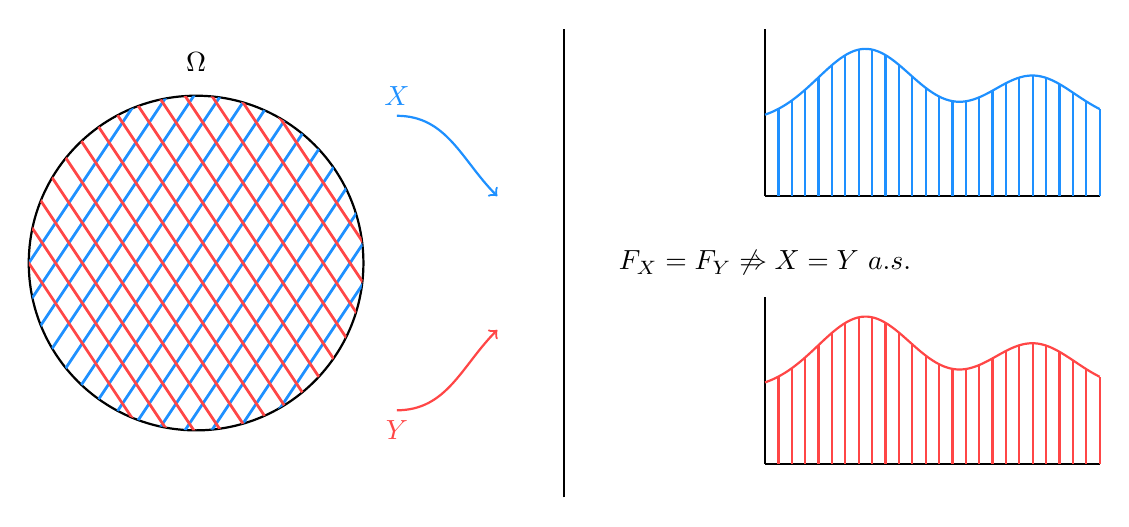
\begin{tikzpicture}[scale=0.85]
      % Define colors
      \definecolor{xcolor}{RGB}{30,144,255}  % Blue
      \definecolor{ycolor}{RGB}{255,70,70}   % Red
      
      % Load patterns library
      \usetikzlibrary{patterns}
      
      % Probability space (Omega)
      \begin{scope}
        \node at (-3.5,3) {$\Omega$};
        \draw[thick] (-3.5,0) circle (2.5);
        
        % Create custom patterns with proper colors and denser lines
        \begin{scope}
          % Blue lines pattern (X) - with reduced spacing between lines
          \clip (-3.5,0) circle (2.5);
          \foreach \i in {-8,-7.6,-7.2,...,5} {
            \draw[xcolor, line width=1.0pt] (\i,-3) -- (\i+4,3);
          }
        \end{scope}
        
        \begin{scope}
          % Red lines pattern (Y) - with reduced spacing between lines
          \clip (-3.5,0) circle (2.5);
          \foreach \i in {-8,-7.6,-7.2,...,2} {
            \draw[ycolor, line width=1.0pt] (\i+4,-3) -- (\i,3);
          }
        \end{scope}
      \end{scope}
      
      % X random variable label and arrow
      \node[xcolor] at (-0.5,2.5) {$X$};
      \draw[->, xcolor, thick, out=0, in=135] (-0.5,2.2) to (1,1);
      
      % Y random variable label and arrow
      \node[ycolor] at (-0.5,-2.5) {$Y$};
      \draw[->, ycolor, thick, out=0, in=225] (-0.5,-2.2) to (1,-1);
      
      % Vertical dividing line
      \draw[thick] (2,-3.5) -- (2,3.5);
      
      % Define distribution function once to ensure consistency
      \pgfmathdeclarefunction{distfunc}{1}{%
        \pgfmathparse{0.1+1.1*exp(-(#1-1.5)^2/1.0)+0.7*exp(-(#1-4)^2/0.8)}%
      }
      
      % X distribution (top right)
      \begin{scope}[shift={(5,2)}]
        \draw[thick] (0,-1) -- (5,-1);
        \draw[thick] (0,-1) -- (0,1.5);
        
        % Calculate curve points directly from the function to ensure alignment
        \draw[xcolor, thick] plot[smooth, domain=0:5, samples=50] 
          (\x, {distfunc(\x)});
        
        % Vertical lines for X distribution
        \foreach \i in {0.2,0.4,...,5} {
          \pgfmathsetmacro{\yval}{distfunc(\i)}
          \draw[xcolor, line width=0.8pt] (\i,-1) -- (\i,\yval);
        }
      \end{scope}
      
      % Relationship text
      \node at (5,0) {$F_X = F_Y \not\Rightarrow X=Y\ a.s.$};
      
      % Y distribution (bottom right)
      \begin{scope}[shift={(5,-2)}]
        \draw[thick] (0,-1) -- (5,-1);
        \draw[thick] (0,-1) -- (0,1.5);
        
        % Calculate curve points directly from the function to ensure alignment
        \draw[ycolor, thick] plot[smooth, domain=0:5, samples=50] 
          (\x, {distfunc(\x)});
        
        % Vertical lines for Y distribution
        \foreach \i in {0.2,0.4,...,5} {
          \pgfmathsetmacro{\yval}{distfunc(\i)}
          \draw[ycolor, line width=0.8pt] (\i,-1) -- (\i,\yval);
        }
      \end{scope}
    \end{tikzpicture}
    \caption{Two identical distributions may not model the same phenomenon.} 
    \label{fig:prob_in_dist}
  \end{figure}

  \begin{theorem}[Hierarchy of Convergence]
    \label{thm:hierarchy-of-convergence}
    Let $X_n, X$ be \hyperref[def:random-variable]{random variables} on $(\Omega, \mathcal{F}, \mathbb{P})$. Then, 
    \begin{equation}
      \text{pointwise c.} \implies \text{almost sure c.} \implies \text{c. in probability} \implies \text{c. in distribution}
    \end{equation}
    Furthermore, if $X_n \xrightarrow{i.p.} X$, then some subsequence $X_{n_k} \xrightarrow{a.s.} X$. 
  \end{theorem}
  \begin{proof}
    \textit{Pointwise $\implies$ almost sure}: the set where $X_n \to X$ is all of $\Omega$, which has probability $1$. 

    \textit{Almost sure $\implies$ in probability}: since $\mathbb{P}(\Omega) = 1 < \infty$, this is \hyperref[mt-thm:egorovs-theorem]{Egorov's theorem} from the measure theory notes (almost everywhere convergence implies convergence in measure on a set of finite measure). 

    \textit{In probability $\implies$ in distribution}: let $x$ be a continuity point of $F_X$ and $\epsilon > 0$. Then $\{X \leq x - \epsilon\} \subset \{X_n \leq x\} \cup \{|X_n - X| > \epsilon\}$ and $\{X_n \leq x\} \subset \{X \leq x + \epsilon\} \cup \{|X_n - X| > \epsilon\}$, so 
    \begin{equation}
      F_X (x - \epsilon) - \mathbb{P}(|X_n - X| > \epsilon) \leq F_{X_n} (x) \leq F_X (x + \epsilon) + \mathbb{P}(|X_n - X| > \epsilon)
    \end{equation}
    Letting $n \to \infty$ and then $\epsilon \to 0$, continuity of $F_X$ at $x$ gives $F_{X_n} (x) \to F_X (x)$. 

    The statement on subsequences is \hyperref[mt-thm:riesz]{Riesz's theorem} from the measure theory notes. 
  \end{proof}

  \begin{example}[Convergence in Probability of $\Exponential(n)$]
    \label{ex:convergence-in-probability-of-exponentialn}
    Given $X_n \sim \Exponential(n)$ with $f_{X_n} (x) = n e^{-nx}$, we show that the sequence converges in probability to the $0$ \hyperref[def:random-variable]{random variable}. Given $\epsilon > 0$, we have 
    \begin{align*}
      \lim_{n \rightarrow \infty} \mathbb{P}(|X_n - 0| > \epsilon) & = \lim_{n \rightarrow \infty} \mathbb{P}(X_n > \epsilon \cup X_n < -\epsilon) \\
      & = \lim_{n \rightarrow \infty} \mathbb{P}(X_n > \epsilon) \\
      & = \lim_{n \rightarrow \infty} \int_\epsilon^\infty n e^{-nx} \,dx \\
      & = \lim_{n \rightarrow \infty} e^{-n \epsilon} = 0
    \end{align*}
    We can imagine this since given any small $\epsilon > 0$, we can see that increasing $n$ results in the distribution of $X_n$ to decrease at a faster rate, and thus a bigger portion of the distribution would lie within $\epsilon$ of the $0$ random variable. 
    \begin{center}
      \captionsetup{type=figure}
      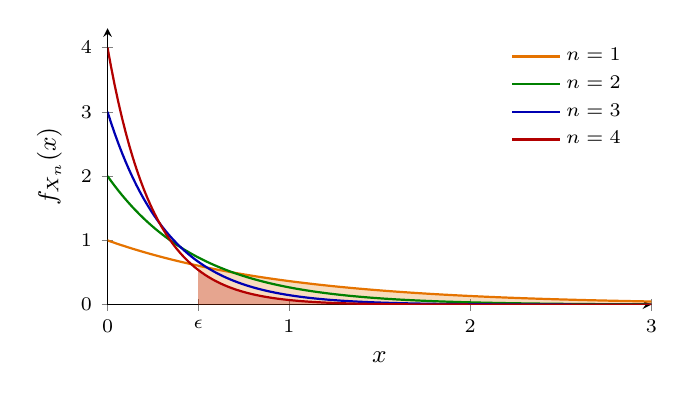
\begin{tikzpicture}
        \begin{axis}[width=0.7\linewidth, height=0.42\linewidth, axis lines=left, xmin=0, xmax=3, ymin=0, ymax=4.3, xlabel={$x$}, ylabel={$f_{X_n} (x)$}, xtick={0,0.5,1,2,3}, xticklabels={$0$,$\epsilon$,$1$,$2$,$3$}, ytick={0,1,2,3,4}, tick label style={font=\scriptsize}, label style={font=\small}, legend style={font=\scriptsize, draw=none, fill=none}, legend pos=north east]
        \addplot[draw=none, fill=orange!90!black, fill opacity=0.25, forget plot] coordinates {(0.5,0) (0.5,0.60653) (0.51667,0.59651) (0.53333,0.58665) (0.55,0.57695) (0.56667,0.56741) (0.58333,0.55804) (0.6,0.54881) (0.61667,0.53974) (0.63333,0.53082) (0.65,0.52205) (0.66667,0.51342) (0.68333,0.50493) (0.7,0.49659) (0.71667,0.48838) (0.73333,0.48031) (0.75,0.47237) (0.76667,0.46456) (0.78333,0.45688) (0.8,0.44933) (0.81667,0.4419) (0.83333,0.4346) (0.85,0.42741) (0.86667,0.42035) (0.88333,0.4134) (0.9,0.40657) (0.91667,0.39985) (0.93333,0.39324) (0.95,0.38674) (0.96667,0.38035) (0.98333,0.37406) (1,0.36788) (1.01667,0.3618) (1.03333,0.35582) (1.05,0.34994) (1.06667,0.34415) (1.08333,0.33847) (1.1,0.33287) (1.11667,0.32737) (1.13333,0.32196) (1.15,0.31664) (1.16667,0.3114) (1.18333,0.30626) (1.2,0.30119) (1.21667,0.29622) (1.23333,0.29132) (1.25,0.2865) (1.26667,0.28177) (1.28333,0.27711) (1.3,0.27253) (1.31667,0.26803) (1.33333,0.2636) (1.35,0.25924) (1.36667,0.25496) (1.38333,0.25074) (1.4,0.2466) (1.41667,0.24252) (1.43333,0.23851) (1.45,0.23457) (1.46667,0.23069) (1.48333,0.22688) (1.5,0.22313) (1.51667,0.21944) (1.53333,0.21582) (1.55,0.21225) (1.56667,0.20874) (1.58333,0.20529) (1.6,0.2019) (1.61667,0.19856) (1.63333,0.19528) (1.65,0.19205) (1.66667,0.18888) (1.68333,0.18575) (1.7,0.18268) (1.71667,0.17966) (1.73333,0.17669) (1.75,0.17377) (1.76667,0.1709) (1.78333,0.16808) (1.8,0.1653) (1.81667,0.16257) (1.83333,0.15988) (1.85,0.15724) (1.86667,0.15464) (1.88333,0.15208) (1.9,0.14957) (1.91667,0.1471) (1.93333,0.14467) (1.95,0.14227) (1.96667,0.13992) (1.98333,0.13761) (2,0.13534) (2.01667,0.1331) (2.03333,0.1309) (2.05,0.12873) (2.06667,0.12661) (2.08333,0.12451) (2.1,0.12246) (2.11667,0.12043) (2.13333,0.11844) (2.15,0.11648) (2.16667,0.11456) (2.18333,0.11267) (2.2,0.1108) (2.21667,0.10897) (2.23333,0.10717) (2.25,0.1054) (2.26667,0.10366) (2.28333,0.10194) (2.3,0.10026) (2.31667,0.0986) (2.33333,0.09697) (2.35,0.09537) (2.36667,0.09379) (2.38333,0.09224) (2.4,0.09072) (2.41667,0.08922) (2.43333,0.08774) (2.45,0.08629) (2.46667,0.08487) (2.48333,0.08346) (2.5,0.08208) (2.51667,0.08073) (2.53333,0.07939) (2.55,0.07808) (2.56667,0.07679) (2.58333,0.07552) (2.6,0.07427) (2.61667,0.07305) (2.63333,0.07184) (2.65,0.07065) (2.66667,0.06948) (2.68333,0.06833) (2.7,0.06721) (2.71667,0.06609) (2.73333,0.065) (2.75,0.06393) (2.76667,0.06287) (2.78333,0.06183) (2.8,0.06081) (2.81667,0.0598) (2.83333,0.05882) (2.85,0.05784) (2.86667,0.05689) (2.88333,0.05595) (2.9,0.05502) (2.91667,0.05411) (2.93333,0.05322) (2.95,0.05234) (2.96667,0.05147) (2.98333,0.05062) (3,0.04979) (3,0)} \closedcycle;
        \addplot[draw=none, fill=red!70!black, fill opacity=0.25, forget plot] coordinates {(0.5,0) (0.5,0.54134) (0.51667,0.50643) (0.53333,0.47377) (0.55,0.44321) (0.56667,0.41463) (0.58333,0.38789) (0.6,0.36287) (0.61667,0.33947) (0.63333,0.31758) (0.65,0.29709) (0.66667,0.27793) (0.68333,0.26001) (0.7,0.24324) (0.71667,0.22755) (0.73333,0.21288) (0.75,0.19915) (0.76667,0.1863) (0.78333,0.17429) (0.8,0.16305) (0.81667,0.15253) (0.83333,0.1427) (0.85,0.13349) (0.86667,0.12488) (0.88333,0.11683) (0.9,0.10929) (0.91667,0.10225) (0.93333,0.09565) (0.95,0.08948) (0.96667,0.08371) (0.98333,0.07831) (1,0.07326) (1.01667,0.06854) (1.03333,0.06412) (1.05,0.05998) (1.06667,0.05611) (1.08333,0.05249) (1.1,0.04911) (1.11667,0.04594) (1.13333,0.04298) (1.15,0.04021) (1.16667,0.03761) (1.18333,0.03519) (1.2,0.03292) (1.21667,0.0308) (1.23333,0.02881) (1.25,0.02695) (1.26667,0.02521) (1.28333,0.02359) (1.3,0.02207) (1.31667,0.02064) (1.33333,0.01931) (1.35,0.01807) (1.36667,0.0169) (1.38333,0.01581) (1.4,0.01479) (1.41667,0.01384) (1.43333,0.01295) (1.45,0.01211) (1.46667,0.01133) (1.48333,0.0106) (1.5,0.00992) (1.51667,0.00928) (1.53333,0.00868) (1.55,0.00812) (1.56667,0.00759) (1.58333,0.0071) (1.6,0.00665) (1.61667,0.00622) (1.63333,0.00582) (1.65,0.00544) (1.66667,0.00509) (1.68333,0.00476) (1.7,0.00446) (1.71667,0.00417) (1.73333,0.0039) (1.75,0.00365) (1.76667,0.00341) (1.78333,0.00319) (1.8,0.00299) (1.81667,0.00279) (1.83333,0.00261) (1.85,0.00245) (1.86667,0.00229) (1.88333,0.00214) (1.9,0.002) (1.91667,0.00187) (1.93333,0.00175) (1.95,0.00164) (1.96667,0.00153) (1.98333,0.00143) (2,0.00134) (2.01667,0.00126) (2.03333,0.00117) (2.05,0.0011) (2.06667,0.00103) (2.08333,0.00096) (2.1,0.0009) (2.11667,0.00084) (2.13333,0.00079) (2.15,0.00074) (2.16667,0.00069) (2.18333,0.00064) (2.2,0.0006) (2.21667,0.00056) (2.23333,0.00053) (2.25,0.00049) (2.26667,0.00046) (2.28333,0.00043) (2.3,0.0004) (2.31667,0.00038) (2.33333,0.00035) (2.35,0.00033) (2.36667,0.00031) (2.38333,0.00029) (2.4,0.00027) (2.41667,0.00025) (2.43333,0.00024) (2.45,0.00022) (2.46667,0.00021) (2.48333,0.00019) (2.5,0.00018) (2.51667,0.00017) (2.53333,0.00016) (2.55,0.00015) (2.56667,0.00014) (2.58333,0.00013) (2.6,0.00012) (2.61667,0.00011) (2.63333,0.00011) (2.65,0.0001) (2.66667,0.00009) (2.68333,0.00009) (2.7,0.00008) (2.71667,0.00008) (2.73333,0.00007) (2.75,0.00007) (2.76667,0.00006) (2.78333,0.00006) (2.8,0.00005) (2.81667,0.00005) (2.83333,0.00005) (2.85,0.00004) (2.86667,0.00004) (2.88333,0.00004) (2.9,0.00004) (2.91667,0.00003) (2.93333,0.00003) (2.95,0.00003) (2.96667,0.00003) (2.98333,0.00003) (3,0.00002) (3,0)} \closedcycle;
        \addplot[thick, color=orange!90!black] coordinates {(0,1) (0.02,0.9802) (0.04,0.96079) (0.06,0.94176) (0.08,0.92312) (0.1,0.90484) (0.12,0.88692) (0.14,0.86936) (0.16,0.85214) (0.18,0.83527) (0.2,0.81873) (0.22,0.80252) (0.24,0.78663) (0.26,0.77105) (0.28,0.75578) (0.3,0.74082) (0.32,0.72615) (0.34,0.71177) (0.36,0.69768) (0.38,0.68386) (0.4,0.67032) (0.42,0.65705) (0.44,0.64404) (0.46,0.63128) (0.48,0.61878) (0.5,0.60653) (0.52,0.59452) (0.54,0.58275) (0.56,0.57121) (0.58,0.5599) (0.6,0.54881) (0.62,0.53794) (0.64,0.52729) (0.66,0.51685) (0.68,0.50662) (0.7,0.49659) (0.72,0.48675) (0.74,0.47711) (0.76,0.46767) (0.78,0.45841) (0.8,0.44933) (0.82,0.44043) (0.84,0.43171) (0.86,0.42316) (0.88,0.41478) (0.9,0.40657) (0.92,0.39852) (0.94,0.39063) (0.96,0.38289) (0.98,0.37531) (1,0.36788) (1.02,0.36059) (1.04,0.35345) (1.06,0.34646) (1.08,0.3396) (1.1,0.33287) (1.12,0.32628) (1.14,0.31982) (1.16,0.31349) (1.18,0.30728) (1.2,0.30119) (1.22,0.29523) (1.24,0.28938) (1.26,0.28365) (1.28,0.27804) (1.3,0.27253) (1.32,0.26714) (1.34,0.26185) (1.36,0.25666) (1.38,0.25158) (1.4,0.2466) (1.42,0.24171) (1.44,0.23693) (1.46,0.23224) (1.48,0.22764) (1.5,0.22313) (1.52,0.21871) (1.54,0.21438) (1.56,0.21014) (1.58,0.20598) (1.6,0.2019) (1.62,0.1979) (1.64,0.19398) (1.66,0.19014) (1.68,0.18637) (1.7,0.18268) (1.72,0.17907) (1.74,0.17552) (1.76,0.17204) (1.78,0.16864) (1.8,0.1653) (1.82,0.16203) (1.84,0.15882) (1.86,0.15567) (1.88,0.15259) (1.9,0.14957) (1.92,0.14661) (1.94,0.1437) (1.96,0.14086) (1.98,0.13807) (2,0.13534) (2.02,0.13266) (2.04,0.13003) (2.06,0.12745) (2.08,0.12493) (2.1,0.12246) (2.12,0.12003) (2.14,0.11765) (2.16,0.11533) (2.18,0.11304) (2.2,0.1108) (2.22,0.10861) (2.24,0.10646) (2.26,0.10435) (2.28,0.10228) (2.3,0.10026) (2.32,0.09827) (2.34,0.09633) (2.36,0.09442) (2.38,0.09255) (2.4,0.09072) (2.42,0.08892) (2.44,0.08716) (2.46,0.08543) (2.48,0.08374) (2.5,0.08208) (2.52,0.08046) (2.54,0.07887) (2.56,0.0773) (2.58,0.07577) (2.6,0.07427) (2.62,0.0728) (2.64,0.07136) (2.66,0.06995) (2.68,0.06856) (2.7,0.06721) (2.72,0.06587) (2.74,0.06457) (2.76,0.06329) (2.78,0.06204) (2.8,0.06081) (2.82,0.05961) (2.84,0.05843) (2.86,0.05727) (2.88,0.05613) (2.9,0.05502) (2.92,0.05393) (2.94,0.05287) (2.96,0.05182) (2.98,0.05079) (3,0.04979)};
        \addlegendentry{$n = 1$}
        \addplot[thick, color=green!50!black] coordinates {(0,2) (0.02,1.92158) (0.04,1.84623) (0.06,1.77384) (0.08,1.70429) (0.1,1.63746) (0.12,1.57326) (0.14,1.51157) (0.16,1.4523) (0.18,1.39535) (0.2,1.34064) (0.22,1.28807) (0.24,1.23757) (0.26,1.18904) (0.28,1.14242) (0.3,1.09762) (0.32,1.05458) (0.34,1.01323) (0.36,0.9735) (0.38,0.93533) (0.4,0.89866) (0.42,0.86342) (0.44,0.82957) (0.46,0.79704) (0.48,0.76579) (0.5,0.73576) (0.52,0.70691) (0.54,0.67919) (0.56,0.65256) (0.58,0.62697) (0.6,0.60239) (0.62,0.57877) (0.64,0.55607) (0.66,0.53427) (0.68,0.51332) (0.7,0.49319) (0.72,0.47386) (0.74,0.45528) (0.76,0.43742) (0.78,0.42027) (0.8,0.40379) (0.82,0.38796) (0.84,0.37275) (0.86,0.35813) (0.88,0.34409) (0.9,0.3306) (0.92,0.31763) (0.94,0.30518) (0.96,0.29321) (0.98,0.28172) (1,0.27067) (1.02,0.26006) (1.04,0.24986) (1.06,0.24006) (1.08,0.23065) (1.1,0.22161) (1.12,0.21292) (1.14,0.20457) (1.16,0.19655) (1.18,0.18884) (1.2,0.18144) (1.22,0.17432) (1.24,0.16749) (1.26,0.16092) (1.28,0.15461) (1.3,0.14855) (1.32,0.14272) (1.34,0.13713) (1.36,0.13175) (1.38,0.12658) (1.4,0.12162) (1.42,0.11685) (1.44,0.11227) (1.46,0.10787) (1.48,0.10364) (1.5,0.09957) (1.52,0.09567) (1.54,0.09192) (1.56,0.08831) (1.58,0.08485) (1.6,0.08152) (1.62,0.07833) (1.64,0.07526) (1.66,0.07231) (1.68,0.06947) (1.7,0.06675) (1.72,0.06413) (1.74,0.06161) (1.76,0.0592) (1.78,0.05688) (1.8,0.05465) (1.82,0.0525) (1.84,0.05045) (1.86,0.04847) (1.88,0.04657) (1.9,0.04474) (1.92,0.04299) (1.94,0.0413) (1.96,0.03968) (1.98,0.03813) (2,0.03663) (2.02,0.03519) (2.04,0.03381) (2.06,0.03249) (2.08,0.03122) (2.1,0.02999) (2.12,0.02882) (2.14,0.02769) (2.16,0.0266) (2.18,0.02556) (2.2,0.02455) (2.22,0.02359) (2.24,0.02267) (2.26,0.02178) (2.28,0.02092) (2.3,0.0201) (2.32,0.01932) (2.34,0.01856) (2.36,0.01783) (2.38,0.01713) (2.4,0.01646) (2.42,0.01581) (2.44,0.01519) (2.46,0.0146) (2.48,0.01403) (2.5,0.01348) (2.52,0.01295) (2.54,0.01244) (2.56,0.01195) (2.58,0.01148) (2.6,0.01103) (2.62,0.0106) (2.64,0.01018) (2.66,0.00979) (2.68,0.0094) (2.7,0.00903) (2.72,0.00868) (2.74,0.00834) (2.76,0.00801) (2.78,0.0077) (2.8,0.0074) (2.82,0.00711) (2.84,0.00683) (2.86,0.00656) (2.88,0.0063) (2.9,0.00606) (2.92,0.00582) (2.94,0.00559) (2.96,0.00537) (2.98,0.00516) (3,0.00496)};
        \addlegendentry{$n = 2$}
        \addplot[thick, color=blue!70!black] coordinates {(0,3) (0.02,2.82529) (0.04,2.66076) (0.06,2.50581) (0.08,2.35988) (0.1,2.22245) (0.12,2.09303) (0.14,1.97114) (0.16,1.85635) (0.18,1.74824) (0.2,1.64643) (0.22,1.55055) (0.24,1.46026) (0.26,1.37522) (0.28,1.29513) (0.3,1.21971) (0.32,1.14868) (0.34,1.08178) (0.36,1.01879) (0.38,0.95946) (0.4,0.90358) (0.42,0.85096) (0.44,0.80141) (0.46,0.75474) (0.48,0.71078) (0.5,0.66939) (0.52,0.63041) (0.54,0.5937) (0.56,0.55912) (0.58,0.52656) (0.6,0.4959) (0.62,0.46702) (0.64,0.43982) (0.66,0.41421) (0.68,0.39009) (0.7,0.36737) (0.72,0.34598) (0.74,0.32583) (0.76,0.30685) (0.78,0.28898) (0.8,0.27215) (0.82,0.2563) (0.84,0.24138) (0.86,0.22732) (0.88,0.21408) (0.9,0.20162) (0.92,0.18988) (0.94,0.17882) (0.96,0.1684) (0.98,0.1586) (1,0.14936) (1.02,0.14066) (1.04,0.13247) (1.06,0.12476) (1.08,0.11749) (1.1,0.11065) (1.12,0.10421) (1.14,0.09814) (1.16,0.09242) (1.18,0.08704) (1.2,0.08197) (1.22,0.0772) (1.24,0.0727) (1.26,0.06847) (1.28,0.06448) (1.3,0.06073) (1.32,0.05719) (1.34,0.05386) (1.36,0.05072) (1.38,0.04777) (1.4,0.04499) (1.42,0.04237) (1.44,0.0399) (1.46,0.03758) (1.48,0.03539) (1.5,0.03333) (1.52,0.03139) (1.54,0.02956) (1.56,0.02784) (1.58,0.02622) (1.6,0.02469) (1.62,0.02325) (1.64,0.0219) (1.66,0.02062) (1.68,0.01942) (1.7,0.01829) (1.72,0.01723) (1.74,0.01622) (1.76,0.01528) (1.78,0.01439) (1.8,0.01355) (1.82,0.01276) (1.84,0.01202) (1.86,0.01132) (1.88,0.01066) (1.9,0.01004) (1.92,0.00945) (1.94,0.0089) (1.96,0.00838) (1.98,0.0079) (2,0.00744) (2.02,0.007) (2.04,0.0066) (2.06,0.00621) (2.08,0.00585) (2.1,0.00551) (2.12,0.00519) (2.14,0.00489) (2.16,0.0046) (2.18,0.00433) (2.2,0.00408) (2.22,0.00384) (2.24,0.00362) (2.26,0.00341) (2.28,0.00321) (2.3,0.00302) (2.32,0.00285) (2.34,0.00268) (2.36,0.00253) (2.38,0.00238) (2.4,0.00224) (2.42,0.00211) (2.44,0.00199) (2.46,0.00187) (2.48,0.00176) (2.5,0.00166) (2.52,0.00156) (2.54,0.00147) (2.56,0.00139) (2.58,0.00131) (2.6,0.00123) (2.62,0.00116) (2.64,0.00109) (2.66,0.00103) (2.68,0.00097) (2.7,0.00091) (2.72,0.00086) (2.74,0.00081) (2.76,0.00076) (2.78,0.00072) (2.8,0.00067) (2.82,0.00064) (2.84,0.0006) (2.86,0.00056) (2.88,0.00053) (2.9,0.0005) (2.92,0.00047) (2.94,0.00044) (2.96,0.00042) (2.98,0.00039) (3,0.00037)};
        \addlegendentry{$n = 3$}
        \addplot[thick, color=red!70!black] coordinates {(0,4) (0.02,3.69247) (0.04,3.40858) (0.06,3.14651) (0.08,2.9046) (0.1,2.68128) (0.12,2.47513) (0.14,2.28484) (0.16,2.10917) (0.18,1.94701) (0.2,1.79732) (0.22,1.65913) (0.24,1.53157) (0.26,1.41382) (0.28,1.30512) (0.3,1.20478) (0.32,1.11215) (0.34,1.02664) (0.36,0.94771) (0.38,0.87485) (0.4,0.80759) (0.42,0.7455) (0.44,0.68818) (0.46,0.63527) (0.48,0.58643) (0.5,0.54134) (0.52,0.49972) (0.54,0.4613) (0.56,0.42583) (0.58,0.39309) (0.6,0.36287) (0.62,0.33497) (0.64,0.30922) (0.66,0.28545) (0.68,0.2635) (0.7,0.24324) (0.72,0.22454) (0.74,0.20728) (0.76,0.19134) (0.78,0.17663) (0.8,0.16305) (0.82,0.15051) (0.84,0.13894) (0.86,0.12826) (0.88,0.1184) (0.9,0.10929) (0.92,0.10089) (0.94,0.09313) (0.96,0.08597) (0.98,0.07936) (1,0.07326) (1.02,0.06763) (1.04,0.06243) (1.06,0.05763) (1.08,0.0532) (1.1,0.04911) (1.12,0.04533) (1.14,0.04185) (1.16,0.03863) (1.18,0.03566) (1.2,0.03292) (1.22,0.03039) (1.24,0.02805) (1.26,0.02589) (1.28,0.0239) (1.3,0.02207) (1.32,0.02037) (1.34,0.0188) (1.36,0.01736) (1.38,0.01602) (1.4,0.01479) (1.42,0.01365) (1.44,0.0126) (1.46,0.01164) (1.48,0.01074) (1.5,0.00992) (1.52,0.00915) (1.54,0.00845) (1.56,0.0078) (1.58,0.0072) (1.6,0.00665) (1.62,0.00614) (1.64,0.00566) (1.66,0.00523) (1.68,0.00483) (1.7,0.00446) (1.72,0.00411) (1.74,0.0038) (1.76,0.0035) (1.78,0.00324) (1.8,0.00299) (1.82,0.00276) (1.84,0.00254) (1.86,0.00235) (1.88,0.00217) (1.9,0.002) (1.92,0.00185) (1.94,0.00171) (1.96,0.00157) (1.98,0.00145) (2,0.00134) (2.02,0.00124) (2.04,0.00114) (2.06,0.00106) (2.08,0.00097) (2.1,0.0009) (2.12,0.00083) (2.14,0.00077) (2.16,0.00071) (2.18,0.00065) (2.2,0.0006) (2.22,0.00056) (2.24,0.00051) (2.26,0.00047) (2.28,0.00044) (2.3,0.0004) (2.32,0.00037) (2.34,0.00034) (2.36,0.00032) (2.38,0.00029) (2.4,0.00027) (2.42,0.00025) (2.44,0.00023) (2.46,0.00021) (2.48,0.0002) (2.5,0.00018) (2.52,0.00017) (2.54,0.00015) (2.56,0.00014) (2.58,0.00013) (2.6,0.00012) (2.62,0.00011) (2.64,0.0001) (2.66,0.0001) (2.68,0.00009) (2.7,0.00008) (2.72,0.00008) (2.74,0.00007) (2.76,0.00006) (2.78,0.00006) (2.8,0.00005) (2.82,0.00005) (2.84,0.00005) (2.86,0.00004) (2.88,0.00004) (2.9,0.00004) (2.92,0.00003) (2.94,0.00003) (2.96,0.00003) (2.98,0.00003) (3,0.00002)};
        \addlegendentry{$n = 4$}
        \end{axis}
      \end{tikzpicture}
      \caption{The PDFs of $X_n \sim \Exponential(n)$ for $n = 1, 2, 3, 4$. The shaded areas to the right of $\epsilon$ are $\mathbb{P}(|X_n - 0| > \epsilon)$ for $n = 1$ (large) and $n = 4$ (small); they shrink to $0$ as $n$ increases.}
      \label{fig:exponential-convergence-in-probability}
    \end{center}
  \end{example}

  \begin{example}[C. in Distribution $\centernot\implies$ C. in Probability]
    \label{ex:c-in-distribution-centernotimplies-c-in}
    Let $X_1, X_2, \ldots$ be such that $X_i = X$ for all $i$ where $X \sim \Bernoulli(1/2)$. This does not mean that the $X_i$'s are iid Bernoulli; they are all copies of the same $X$, i.e. forms a constant sequence. Let $Y = 1 - X$. Clearly, $X_n \xrightarrow{D} Y$ since the CDF of every $X_i$ is the same as that of $Y$, but $|X_n - Y| = 1$ for all $n$, so there is no convergence.  
  \end{example}

  \begin{example}[C. in Distribution $\centernot\implies$ C. in Probability]
    \label{ex:c-in-distribution-centernotimplies-c-in-2}
    Let $X_1, X_2, \ldots \sim \mathcal{N}(0, 1)$ and $Y = -X$. Then, by symmetry of the standard Gaussian, both $X$ and $Y$ have the same CDF, but they are not the same \hyperref[def:random-variable]{random variable}: their signs are opposite. 
  \end{example}

  Convergence almost surely and convergence with probability are very different. \hyperref[mt-def:almost-sure-convergence]{Almost sure convergence} has the limit inside the probability, which indicates that we are talking about convergence of a sequence of \hyperref[def:random-variable]{random variables}. On the other hand, convergence in probability has the limit on the outside, which talks about convergence of a sequence of probabilities. But a key point is that almost sure convergence implies convergence in probability. It happens so because there could exist a subset of small probability in $\Omega$ where the $X_n$'s and $X$ need not be close, but the probabilities of them deviating over whole $\Omega$ is small. 

  \begin{example}[C. in Probability $\centernot\implies$ C. Almost Surely]
    \label{ex:c-in-probability-centernotimplies-c-almost-2}
    Let us take the sequence $X_1, X_2, \ldots$ of \hyperref[def:independent-random-variables]{independent random variables} where $X_n \sim \Bernoulli(1/n)$. That is, 
    \begin{equation}
      \mathbb{P}(X_n = 1) = \frac{1}{n} \text{ and } \mathbb{P}(X_n = 0) = 1 - \frac{1}{n}
    \end{equation}
    So, as $n$ gets large we expect $X_n$ to realize values of $0$ more and more. Showing that $X_n \xrightarrow{i.p.} 0$ is easy, since we can compute for any $\epsilon > 0$
    \begin{align*}
      \lim_{n \rightarrow \infty} \mathbb{P}(|X_n - 0| > \epsilon) & = \lim_{n \rightarrow \infty} \mathbb{P}(|X_n| > \epsilon) \\
      & = \lim_{n \rightarrow \infty} \mathbb{P}(X_n = 1) \\
      & = \lim_{n \rightarrow \infty} \frac{1}{n} = 0
    \end{align*}
    We want to show that this does not converge almost surely to $0$, i.e. there is some set of nonzero measure such that for some $\omega$ in that set, the sequence $X_1 (\omega), X_2(\omega), \ldots$ does not converge to $0$. This can be hard to see at first, but the fact that we have independence and the terms are $\frac{1}{n}$ hints at the \hyperref[mt-thm:borel-cantelli-lemma]{Borel-Cantelli lemma}. Let $A_n$ be the event that $\{X_n = 1\}$ (i.e. the preimage of the singleton set under $X_n$: $X_n^{-1} ( \{1\})$). Then, the $A_n$'s are independent, and 
    \begin{equation}
      \sum_{n=1}^\infty \mathbb{P}(A_n) = +\infty
    \end{equation}
    By the Borel-Cantelli lemma 2, this implies that almost surely infinitely many $A_n$'s will occur. That is, we can choose as large of an $n$ as we like, go down the sequence until we look at $X_n, X_{n+1}, \ldots$, and we are guaranteed with probability $1$ that at least one of the $X_i$'s after $n$ will realize a $1$. This means that in every realization of $X_1, X_2, \ldots$, we will get a sequence of $0$s and $1$s, but since BCL states that no matter how far down the road you will always get at least another $1$, this sequence does not converge to $0$.  
  \end{example}

  A sequence like the one above, or the ``typewriter'' sequence of indicator functions in the \hyperref[mt-def:convergence-in-measure]{measure theory notes}, satisfies convergence in probability as follows: As $n$ increases, $X_n$ is more and more likely to be near $X$ (in the way that $|X_n - X| < \epsilon$ for some $\epsilon > 0$), ultimately satisfying this closeness property with probability $1$ as $n \rightarrow \infty$. For example, we could have 
  \begin{align*}
    \mathbb{P}(|X_1 - X| > \epsilon) & = 1 \\
    \mathbb{P}(|X_2 - X| > \epsilon) & = 1/2 \\
    \mathbb{P}(|X_3 - X| > \epsilon) & = 1/3 \\
    \ldots & = \ldots 
  \end{align*}
  This definitely satisfies convergence in probability, but this leaves open the possibility that $\mathbb{P}(|X_n - X| > \epsilon)$ an infinite number of times, although at infrequent intervals. Therefore, when looking at the sequence 
  \begin{equation}
    X_1, X_2, X_3, \ldots
  \end{equation}
  each random variable \textit{individually} may have less chance of being more than $\epsilon$ away from $X$, but since there is an infinite number of them in the sequence, the sequence \textit{in totality} may contain an infinite number of cases where $|X_n - X| > \epsilon$. Convergence almost surely tells us that we are \textit{guaranteed} (with probability $1$) that this sequence will converge to $X$. That is, we can specify an $N \in \mathbb{N}$ such that $|X_n - X| < \epsilon$ for all $n > N$. 

  Let us define some $\epsilon > 0$ and consider a sequence of random variables $\{X_n\}_{n \in \mathbb{N}}$. Given some outcome $\omega \in \Omega$, we will consider it a \textit{success} if $|X_n(\omega) - X(\omega)| < \epsilon$ and \textit{failure} if not. Then, convergence in probability tells us that the probability of failure goes to $0$ as $n$ goes to infinity and therefore we get better and better estimates of $X$. Convergence almost surely is a bit stronger and says that the total number of failures is \textit{finite}. That is, after a certain point $N$, the random variable $X_n$ will \textit{always} estimate $X$ within an error of $\epsilon$ (i.e. such that $|X_n - X| < \epsilon$). But since you don't know when you've exhausted all failures, there is not much of a difference from a practical point of view. 

  \begin{definition}[Joint Cumulative Distribution Function]
    \label{def:joint-cumulative-distribution-function}
    Since sets of the form $(-\infty, x] \times (-\infty, y]$ are Borel in $\mathbb{R}^2$, the \textbf{joint cumulative distribution function} 
    \begin{align*}
      F_{X, Y} & \coloneqq \mathbb{P}_{X, Y} \big( (-\infty, x] \times (-\infty, y] \big) \\
      & = \mathbb{P} \big( \{\omega \mid X(\omega) \leq x\} \cap \{ \omega \mid Y(\omega) \leq y\} \big)
    \end{align*}
    is well-defined. We will also write $F_{X, Y} (x, y) = \mathbb{P}(X \leq x, Y \leq y)$. The marginal CDFs are defined 
    \begin{align*}
      F_X (x) & \coloneqq \mathbb{P}_{X, Y} ((-\infty, x) \times \mathbb{R}) \\
      F_Y (y) & \coloneqq \mathbb{P}_{X, Y} (\mathbb{R} \times (-\infty, y))
    \end{align*}
  \end{definition}

  \begin{lemma}[Properties of Joint CDF]
    \label{thm:properties-of-joint-cdf}
    Some common properties of the joint CDF are as follows: 
    \begin{enumerate}
      \item Limits. 
      \begin{equation}
        \lim_{(x, y) \rightarrow (+\infty, +\infty)} F_{X, Y} (x, y) = 1 \text{ and } \lim_{(x, y) \rightarrow (-\infty, -\infty)} F_{X, Y} (x, y) = 0
      \end{equation}
      \item Monotonicity. 
      \begin{equation}
        x_1 \leq x_2, \; y_1 \leq y_2 \implies F_{X, Y} (x_1, y_1) \leq F_{X, Y}(x_2, y_2)
      \end{equation}
      \item Continuity from above. 
      \begin{equation}
        \lim_{\epsilon \rightarrow 0^+} F_{X, Y} (x + \epsilon, y + \epsilon) = F_{X, Y} (x, y) \text{ for all } x, y \in \mathbb{R}
      \end{equation}
      \item Maringal CDFs. 
      \begin{equation}
        \lim_{y \rightarrow \infty} F_{X, Y} (x, y) = F_X (x), \;\;\;\; \lim_{x \rightarrow \infty} F_{X, Y} (x, y) = F_Y (y)
      \end{equation}
    \end{enumerate}
  \end{lemma}

  If $X, Y$ are independent, then we can say something about the CDFs 

  \begin{theorem}[Independence via the Joint CDF]
    \label{thm:independence-via-the-joint-cdf}
    $X$ and $Y$ are independent RVs if and only if 
    \begin{equation}
      F_{X, Y} (x, y) = F_X (x) \, F_Y (y)
    \end{equation}
  \end{theorem}

\subsection{Densities} 

  You classify \hyperref[def:random-variable]{random variables} based on the nature of the measure $\mathbb{P}_X$ induced on the real line. Note that we can have a continuous \hyperref[def:probability-space]{probability space} $\Omega$ with a discrete random variable $X$ (e.g. coin flips). There are only three fundamental types of measures: discrete, continuous and singular random variables. In fact, a result in measure theory called \textit{Lebesgue's Decomposition Theorem} says that every measure on $\mathbb{R}$ are either one of these 3 or mixtures thereof. We are used to the first two; the third one is very bizzare and has little to no practical applications. 

  Note that if we are working in a \hyperref[def:discrete-probability-space]{discrete probability space} $\Omega$, then we can simply take the $\sigma$-algebra to be $2^\Omega$, and so we can take any function on $\Omega$ as a random variable since its preimage will always be in $2^\Omega$. 

  \begin{definition}[Discrete Random Variable]
    \label{def:discrete-random-variable}
    A \textbf{discrete random variable} is a measurable function $X: (\Omega, \mathcal{F}, \mathbb{P}) \to \mathcal{X}$ into a \hyperref[st-def:countable]{countable set} $\mathcal{X}$ (with the $\sigma$-algebra $2^{\mathcal{X}}$). Its \textbf{probability mass function} (PMF) is 
    \begin{equation}
      p_X (x) \coloneqq \mathbb{P}(X = x) = \mathbb{P}_X (\{x\}), \qquad x \in \mathcal{X}
    \end{equation}
    Then $\sum_{x \in \mathcal{X}} p_X (x) = 1$, and the PMF determines the entire probability law: for every $B \subset \mathcal{X}$, 
    \begin{equation}
      \mathbb{P}_X (B) = \sum_{x \in B} p_X (x)
    \end{equation}
  \end{definition}
  \begin{proof}
    Since $B \subset \mathcal{X}$ is countable, it is the \hyperref[st-def:disjoint-sets]{disjoint} union of its singletons $\{x\}$, and by countable additivity, 
    \begin{equation}
      \mathbb{P}_X (B) = \mathbb{P}_X \bigg( \bigsqcup_{x \in B} \{x\} \bigg) = \sum_{x \in B} \mathbb{P}_X (\{x\}) = \sum_{x \in B} p_X (x)
    \end{equation}
    Taking $B = \mathcal{X}$ gives $\sum_{x \in \mathcal{X}} p_X (x) = \mathbb{P}_X (\mathcal{X}) = 1$. 
  \end{proof}

  For example, $\mathcal{X}$ can be $\{\text{heads}, \text{tails}\}$, or a subset of $\mathbb{R}$. If $X$ is real-valued and only satisfies $\mathbb{P}_X (E) = 1$ for some countable $E \subset \mathbb{R}$ (rather than having a countable image), we can simply take $\mathcal{X} = E$. What's nice about the \hyperref[def:discrete-random-variable]{discrete random variable} is that the probability mass function $p_X$ completely describes its probability law. 

	\begin{figure}[H]
		\centering 
		\begin{tikzpicture}[x=1cm, y=1cm, >=Stealth, scale=0.7]
			\definecolor{cdfblue}{RGB}{30,120,255}

			% ---------- Axes ----------
			\draw[-{Stealth[length=3mm]}, thick] (-0.5,0) -- (13,0);               % x-axis
			\draw[-{Stealth[length=3mm]}, thick] (6.2,-0.3) -- (6.2,5);            % y-axis
			\node[font=\Large\bfseries] at (5.8,4.8) {1};

			% ---------- x positions of e_1,...,e_5 ----------
			\def\ea{0.8}
			\def\eb{2.7}
			\def\ec{5.6}
			\def\ed{7.2}
			\def\ee{9.2}

			% ---------- y levels of the CDF ----------
			\def\ya{0.9}
			\def\yb{1.9}
			\def\yc{3.0}
			\def\yd{3.9}
			\def\ye{4.6}

			% ---------- Tick marks and labels ----------
			\foreach \x/\lab in {\ea/e_1, \eb/e_2, \ec/e_3, \ed/e_4, \ee/e_5}{
				\draw[thick] (\x,0.1) -- (\x,-0.1);
				\node[below, font=\Large] at (\x,-0.15) {$\lab$};
			}

			% ---------- CDF: left arrow along x-axis ----------
			\draw[cdfblue, very thick, -{Stealth[length=3mm]}] (\ea,0) -- (-0.6,0);

			% ---------- CDF: horizontal steps ----------
			\draw[cdfblue, very thick] (\ea,\ya) -- (\eb,\ya);
			\draw[cdfblue, very thick] (\eb,\yb) -- (\ec,\yb);
			\draw[cdfblue, very thick] (\ec,\yc) -- (\ed,\yc);
			\draw[cdfblue, very thick] (\ed,\yd) -- (\ee,\yd);
			\draw[cdfblue, very thick, -{Stealth[length=3mm]}] (\ee,\ye) -- (12.5,\ye);

			% ---------- Dotted vertical jumps ----------
			\draw[cdfblue, thick, dotted] (\ea,0)   -- (\ea,\ya);
			\draw[cdfblue, thick, dotted] (\eb,\ya) -- (\eb,\yb);
			\draw[cdfblue, thick, dotted] (\ec,\yb) -- (\ec,\yc);
			\draw[cdfblue, thick, dotted] (\ed,\yc) -- (\ed,\yd);
			\draw[cdfblue, thick, dotted] (\ee,\yd) -- (\ee,\ye);

			% ---------- Open circles (left limits) ----------
			\foreach \x/\y in {\ea/0, \eb/\ya, \ec/\yb, \ed/\yc, \ee/\yd}{
				\filldraw[fill=white, draw=cdfblue, very thick] (\x,\y) circle (0.09);
			}

			% ---------- Filled dots (right-continuous values) ----------
			\foreach \x/\y in {\ea/\ya, \eb/\yb, \ec/\yc, \ed/\yd, \ee/\ye}{
				\fill[cdfblue] (\x,\y) circle (0.09);
			}

			% ---------- Jump labels ----------
			\node[cdfblue, right, font=\large] at (\ea,0.45)  {$P(X=e_1)$};
			\node[cdfblue, right, font=\large] at (\eb,1.4)   {$P(X=e_2)$};
			\node[cdfblue, right, font=\large] at (\ec,2.45)  {$P(X=e_3)$};
			\node[cdfblue, right, font=\large] at (\ed,3.45)  {$P(X=e_4)$};
			\node[cdfblue, right, font=\large] at (\ee,4.25)  {$P(X=e_5)$};
		\end{tikzpicture}
		\caption{The CDF of a discrete probability function will look like an increasing series of steps. If we have a real-valued $X$ with $\mathcal{X} = \{e_1, e_2, e_3, e_4, e_5\}$, its CDF would look like the following. } 
		\label{fig:discrete_cdf}
	\end{figure}

  If $\mathcal{X} \subset \mathbb{R}$ is countably infinite, then its CDF has countably infinitely many discontinuities. Now we'll give some examples of discrete random variables, and in here we'll completely ignore the sample space $\Omega$, since once we have a \hyperref[def:random-variable]{random variable} $X$, we can just work in $(\mathbb{R}, \mathcal{R}, \mathbb{P}_X)$. Remember that we will write $P(X = x)$ as shorthand for $\mathbb{P}_X (\{x\})$. 

  \pgfplotsset{
    rvplot/.style={width=\linewidth, height=0.8\linewidth, axis lines=left, tick label style={font=\scriptsize, /pgf/number format/fixed}, scaled ticks=false, label style={font=\small}, legend style={font=\scriptsize, draw=none, fill=none}}
  }

  \begin{definition}[Indicator/Bernoulli Random Variable]
    \label{def:indicator-bernoulli-random-variable}
    A \textbf{Bernoulli random variable} $X \sim \Bernoulli(p)$ is a \hyperref[def:discrete-random-variable]{random variable} taking values in $\mathcal{X} = \{0, 1\}$ with PMF 
    \begin{equation}
      \mathbb{P}(X = 1) = p, \qquad \mathbb{P}(X = 0) = 1 - p
    \end{equation}
    where $p \in [0, 1]$. 
    Its CDF is 
    \begin{equation}
      F_X (x) = \begin{cases} 0 & \text{ if } x < 0 \\ 1 - p & \text{ if } 0 \leq x < 1 \\ 1 & \text{ if } 1 \leq x \end{cases}
    \end{equation}
  \begin{center}
    \captionsetup{type=figure}
    \begin{subfigure}[b]{0.48\textwidth}
      \centering
      \begin{tikzpicture}
          \begin{axis}[rvplot, xlabel={$k$}, ylabel={$\mathbb{P}(X = k)$}, ymin=0, ymax=1.0, xmin=-1, xmax=2, xtick={0,1}]
            \addplot+[ycomb, mark=*, mark size=1.8pt, thick, color=blue!70!black, mark options={fill=blue!70!black}] coordinates {(0,0.7) (1,0.3)};
          \end{axis}
      \end{tikzpicture}
      \caption{PMF of a $\Bernoulli(0.3)$ random variable.}
      \label{fig:bernoulli-pmf}
    \end{subfigure}
    \hfill 
    \begin{subfigure}[b]{0.48\textwidth}
      \centering
      \begin{tikzpicture}
          \begin{axis}[rvplot, xlabel={$x$}, ylabel={$F_X (x)$}, ymin=0, ymax=1.05, xmin=-1, xmax=2, xtick={0,1}]
            \addplot+[const plot mark left, mark=*, mark size=1.5pt, thick, color=blue!70!black, mark options={fill=blue!70!black}] coordinates {(-1,0) (0,0.7) (1,1) (2,1)};
          \end{axis}
      \end{tikzpicture}
      \caption{CDF of a $\Bernoulli(0.3)$ random variable.}
      \label{fig:bernoulli-cdf}
    \end{subfigure}
    \caption{The PMF and CDF of a $\Bernoulli(0.3)$ random variable.}
    \label{fig:bernoulli}
  \end{center}
  \end{definition}
  \begin{proof}
    $1_A$ is a random variable since the preimages of $\emptyset, \{0\}, \{1\}, \{0, 1\}$ are $\emptyset, A^c, A, \Omega$, which are all $\mathcal{F}$-measurable. Its PMF is $\mathbb{P}(1_A = 1) = \mathbb{P}(A) = p$ and $\mathbb{P}(1_A = 0) = \mathbb{P}(A^c) = 1 - p$, and the CDF is obtained by summing the PMF over all values $\leq x$. 
  \end{proof}

  \begin{definition}[Discrete Uniform Random Variable]
    \label{def:uniform-random-variable}
    A \textbf{discrete uniform random variable} $X \sim \Uniform(\mathcal{X})$ is a \hyperref[def:discrete-random-variable]{random variable} taking values in a \hyperref[st-def:finite-set]{finite set} $\mathcal{X} = \{x_i\}_{i=1}^n$ with PMF 
    \begin{equation}
      \mathbb{P}(X = x_i) = \frac{1}{n}, \qquad i = 1, 2, \ldots, n
    \end{equation}
    If $\mathcal{X} \subset \mathbb{R}$, its CDF is 
    \begin{equation}
      F_X (x) = \frac{\big| \{ i \mid x_i \leq x \} \big|}{n}
    \end{equation}
  \end{definition}

  The Bernoulli RV leads to the geometric and binomial random variables. 

  \begin{definition}[Geometric Random Variable]
    \label{def:geometric-random-variable}
    A \textbf{geometric random variable} $X \sim \Geometric(p)$ is a \hyperref[def:discrete-random-variable]{random variable} taking values in $\mathcal{X} = \mathbb{N}$ with PMF 
    \begin{equation}
      \mathbb{P}(X = k) = (1 - p)^{k-1} p, \qquad k \in \mathbb{N}
    \end{equation}
    where $p \in (0, 1]$. It is the number of independent tosses of a $p$-coin (probability of heads is $p$) needed to get the first heads. 
    Its CDF is 
    \begin{equation}
      F_X (x) = \begin{cases} 0 & \text{ if } x < 1 \\ 1 - (1 - p)^{\lfloor x \rfloor} & \text{ if } x \geq 1 \end{cases}
    \end{equation}
  \begin{center}
    \captionsetup{type=figure}
    \begin{subfigure}[b]{0.48\textwidth}
      \centering
      \begin{tikzpicture}
          \begin{axis}[rvplot, xlabel={$k$}, ylabel={$\mathbb{P}(X = k)$}, ymin=0, ymax=0.35, xmin=0, xmax=16, xtick={0,5,10,15}]
            \addplot+[ycomb, mark=*, mark size=1.8pt, thick, color=blue!70!black, mark options={fill=blue!70!black}] coordinates {(1,0.3) (2,0.21) (3,0.147) (4,0.1029) (5,0.07203) (6,0.05042) (7,0.03529) (8,0.02471) (9,0.01729) (10,0.01211) (11,0.00847) (12,0.00593) (13,0.00415) (14,0.00291) (15,0.00203)};
          \end{axis}
      \end{tikzpicture}
      \caption{PMF of a $\Geometric(0.3)$ random variable.}
      \label{fig:geometric-pmf}
    \end{subfigure}
    \hfill 
    \begin{subfigure}[b]{0.48\textwidth}
      \centering
      \begin{tikzpicture}
          \begin{axis}[rvplot, xlabel={$x$}, ylabel={$F_X (x)$}, ymin=0, ymax=1.05, xmin=0, xmax=16, xtick={0,5,10,15}]
            \addplot+[const plot mark left, mark=*, mark size=1.5pt, thick, color=blue!70!black, mark options={fill=blue!70!black}] coordinates {(0,0) (1,0.3) (2,0.51) (3,0.657) (4,0.7599) (5,0.83193) (6,0.88235) (7,0.91765) (8,0.94235) (9,0.95965) (10,0.97175) (11,0.98023) (12,0.98616) (13,0.99031) (14,0.99322) (15,0.99525) (16,0.99525)};
          \end{axis}
      \end{tikzpicture}
      \caption{CDF of a $\Geometric(0.3)$ random variable.}
      \label{fig:geometric-cdf}
    \end{subfigure}
    \caption{The PMF and CDF of a $\Geometric(0.3)$ random variable.}
    \label{fig:geometric}
  \end{center}
  \begin{center}
    \captionsetup{type=figure}
    \begin{subfigure}[b]{0.48\textwidth}
      \centering
      \begin{tikzpicture}
          \begin{axis}[rvplot, xlabel={$k$}, ylabel={$\mathbb{P}(X = k)$}, ymin=0, ymax=0.5, xmin=0, xmax=7, xtick={1,2,3,4,5,6}]
            \addplot+[ycomb, mark=*, mark size=1.8pt, thick, color=blue!70!black, mark options={fill=blue!70!black}] coordinates {(1,0.16667) (2,0.16667) (3,0.16667) (4,0.16667) (5,0.16667) (6,0.16667)};
          \end{axis}
      \end{tikzpicture}
      \caption{PMF of a $\Uniform(\{1, \ldots, 6\})$ random variable.}
      \label{fig:discrete-uniform-pmf}
    \end{subfigure}
    \hfill 
    \begin{subfigure}[b]{0.48\textwidth}
      \centering
      \begin{tikzpicture}
          \begin{axis}[rvplot, xlabel={$x$}, ylabel={$F_X (x)$}, ymin=0, ymax=1.05, xmin=0, xmax=7, xtick={1,2,3,4,5,6}]
            \addplot+[const plot mark left, mark=*, mark size=1.5pt, thick, color=blue!70!black, mark options={fill=blue!70!black}] coordinates {(0,0) (1,0.16667) (2,0.33333) (3,0.5) (4,0.66667) (5,0.83333) (6,1) (7,1)};
          \end{axis}
      \end{tikzpicture}
      \caption{CDF of a $\Uniform(\{1, \ldots, 6\})$ random variable.}
      \label{fig:discrete-uniform-cdf}
    \end{subfigure}
    \caption{The PMF and CDF of a $\Uniform(\{1, \ldots, 6\})$ random variable.}
    \label{fig:discrete-uniform}
  \end{center}
  \end{definition}
  \begin{proof}
    The first heads occurs on toss $k$ exactly when the first $k - 1$ tosses are tails and the $k$th is heads, which has probability $(1-p)^{k-1} p$ by independence. This is a valid PMF since by the geometric series, $\sum_{k=1}^\infty (1-p)^{k-1} p = \frac{p}{1 - (1 - p)} = 1$. The CDF is the partial sum $F_X (x) = \sum_{k=1}^{\lfloor x \rfloor} (1-p)^{k-1} p = 1 - (1-p)^{\lfloor x \rfloor}$, which is also $1$ minus the probability that the first $\lfloor x \rfloor$ tosses are all tails. 
  \end{proof}

  \begin{definition}[Binomial Random Variable]
    \label{def:binomial-random-variable}
    A \textbf{binomial random variable} $X \sim \Binomial(n, p)$ is a \hyperref[def:discrete-random-variable]{random variable} taking values in $\mathcal{X} = \{0, 1, \ldots, n\}$ with PMF 
    \begin{equation}
      \mathbb{P}(X = k) = \binom{n}{k} p^k (1 - p)^{n - k}, \qquad k \in \{0, 1, \ldots, n\}
    \end{equation}
    where $n \in \mathbb{N}$ and $p \in [0, 1]$. It is the number of heads in a sequence of $n$ independent tosses of a $p$-coin. 
    Its CDF is 
    \begin{equation}
      F_X (x) = \begin{cases} 0 & \text{ if } x < 0 \\ \sum_{k=0}^{\lfloor x \rfloor} \binom{n}{k} p^k (1 - p)^{n - k} & \text{ if } 0 \leq x < n \\ 1 & \text{ if } x \geq n \end{cases}
    \end{equation}
  \begin{center}
    \captionsetup{type=figure}
    \begin{subfigure}[b]{0.48\textwidth}
      \centering
      \begin{tikzpicture}
          \begin{axis}[rvplot, xlabel={$k$}, ylabel={$\mathbb{P}(X = k)$}, ymin=0, ymax=0.3, xmin=-1, xmax=11, xtick={0,2,4,6,8,10}]
            \addplot+[ycomb, mark=*, mark size=1.8pt, thick, color=blue!70!black, mark options={fill=blue!70!black}] coordinates {(0,0.00605) (1,0.04031) (2,0.12093) (3,0.21499) (4,0.25082) (5,0.20066) (6,0.11148) (7,0.04247) (8,0.01062) (9,0.00157) (10,0.0001)};
          \end{axis}
      \end{tikzpicture}
      \caption{PMF of a $\Binomial(10, 0.4)$ random variable.}
      \label{fig:binomial-pmf}
    \end{subfigure}
    \hfill 
    \begin{subfigure}[b]{0.48\textwidth}
      \centering
      \begin{tikzpicture}
          \begin{axis}[rvplot, xlabel={$x$}, ylabel={$F_X (x)$}, ymin=0, ymax=1.05, xmin=-1, xmax=11, xtick={0,2,4,6,8,10}]
            \addplot+[const plot mark left, mark=*, mark size=1.5pt, thick, color=blue!70!black, mark options={fill=blue!70!black}] coordinates {(-1,0) (0,0.00605) (1,0.04636) (2,0.16729) (3,0.38228) (4,0.6331) (5,0.83376) (6,0.94524) (7,0.98771) (8,0.99832) (9,0.9999) (10,1) (11,1)};
          \end{axis}
      \end{tikzpicture}
      \caption{CDF of a $\Binomial(10, 0.4)$ random variable.}
      \label{fig:binomial-cdf}
    \end{subfigure}
    \caption{The PMF and CDF of a $\Binomial(10, 0.4)$ random variable.}
    \label{fig:binomial}
  \end{center}
  \end{definition}
  \begin{proof}
    Any particular sequence of $n$ tosses with exactly $k$ heads has probability $p^k (1-p)^{n-k}$ by independence, and there are $\binom{n}{k}$ such (disjoint) sequences, one for each choice of the positions of the heads. This is a valid PMF since by the binomial theorem, $\sum_{k=0}^n \binom{n}{k} p^k (1-p)^{n-k} = (p + 1 - p)^n = 1$. 
  \end{proof}

  \begin{definition}[Poisson Random Variable]
    \label{def:poisson-random-variable}
    A \textbf{Poisson random variable} $X \sim \Poisson(\lambda)$ is a \hyperref[def:discrete-random-variable]{random variable} taking values in $\mathcal{X} = \mathbb{N}_0$ with PMF 
    \begin{equation}
      \mathbb{P}(X = k) = \frac{e^{-\lambda} \lambda^k}{k!}, \qquad k \in \mathbb{N}_0
    \end{equation}
    where $\lambda > 0$. 
    Its CDF is 
    \begin{equation}
      F_X (x) = \begin{cases} 0 & \text{ if } x < 0 \\ e^{-\lambda} \sum_{k=0}^{\lfloor x \rfloor} \frac{\lambda^k}{k!} & \text{ if } x \geq 0 \end{cases}
    \end{equation}
  \begin{center}
    \captionsetup{type=figure}
    \begin{subfigure}[b]{0.48\textwidth}
      \centering
      \begin{tikzpicture}
          \begin{axis}[rvplot, xlabel={$k$}, ylabel={$\mathbb{P}(X = k)$}, ymin=0, ymax=0.22, xmin=-1, xmax=15, xtick={0,2,4,6,8,10,12,14}]
            \addplot+[ycomb, mark=*, mark size=1.8pt, thick, color=blue!70!black, mark options={fill=blue!70!black}] coordinates {(0,0.01832) (1,0.07326) (2,0.14653) (3,0.19537) (4,0.19537) (5,0.15629) (6,0.1042) (7,0.05954) (8,0.02977) (9,0.01323) (10,0.00529) (11,0.00192) (12,0.00064) (13,0.0002) (14,0.00006)};
          \end{axis}
      \end{tikzpicture}
      \caption{PMF of a $\Poisson(4)$ random variable.}
      \label{fig:poisson-pmf}
    \end{subfigure}
    \hfill 
    \begin{subfigure}[b]{0.48\textwidth}
      \centering
      \begin{tikzpicture}
          \begin{axis}[rvplot, xlabel={$x$}, ylabel={$F_X (x)$}, ymin=0, ymax=1.05, xmin=-1, xmax=15, xtick={0,2,4,6,8,10,12,14}]
            \addplot+[const plot mark left, mark=*, mark size=1.5pt, thick, color=blue!70!black, mark options={fill=blue!70!black}] coordinates {(-1,0) (0,0.01832) (1,0.09158) (2,0.2381) (3,0.43347) (4,0.62884) (5,0.78513) (6,0.88933) (7,0.94887) (8,0.97864) (9,0.99187) (10,0.99716) (11,0.99908) (12,0.99973) (13,0.99992) (14,0.99998) (15,0.99998)};
          \end{axis}
      \end{tikzpicture}
      \caption{CDF of a $\Poisson(4)$ random variable.}
      \label{fig:poisson-cdf}
    \end{subfigure}
    \caption{The PMF and CDF of a $\Poisson(4)$ random variable.}
    \label{fig:poisson}
  \end{center}
  \end{definition}
  \begin{proof}
    This is a valid PMF since by the Taylor series of the exponential, $\sum_{k=0}^\infty \frac{e^{-\lambda} \lambda^k}{k!} = e^{-\lambda} e^{\lambda} = 1$. 
  \end{proof}

  \begin{definition}[Negative Binomial Random Variable]
    \label{def:negative-binomial-distribution}
    A \textbf{negative binomial random variable} $X \sim \NegBinomial(r, p)$ is a \hyperref[def:discrete-random-variable]{random variable} taking values in $\mathcal{X} = \mathbb{N}_0$ with PMF 
    \begin{equation}
      \mathbb{P}(X = k) = \binom{k+r-1}{k} \, (1-p)^r \, p^k, \qquad k \in \mathbb{N}_0
    \end{equation}
    where $r \in \mathbb{N}$ and $p \in (0, 1)$. It is the number of successes in a sequence of independent Bernoulli-$p$ trials before the $r$th failure. 
    Its CDF is 
    \begin{equation}
      F_X (x) = \begin{cases} 0 & \text{ if } x < 0 \\ \sum_{k=0}^{\lfloor x \rfloor} \binom{k+r-1}{k} (1-p)^r p^k & \text{ if } x \geq 0 \end{cases}
    \end{equation}
  \begin{center}
    \captionsetup{type=figure}
    \begin{subfigure}[b]{0.48\textwidth}
      \centering
      \begin{tikzpicture}
          \begin{axis}[rvplot, xlabel={$k$}, ylabel={$\mathbb{P}(X = k)$}, ymin=0, ymax=0.22, xmin=-1, xmax=15, xtick={0,2,4,6,8,10,12,14}]
            \addplot+[ycomb, mark=*, mark size=1.8pt, thick, color=blue!70!black, mark options={fill=blue!70!black}] coordinates {(0,0.125) (1,0.1875) (2,0.1875) (3,0.15625) (4,0.11719) (5,0.08203) (6,0.05469) (7,0.03516) (8,0.02197) (9,0.01343) (10,0.00806) (11,0.00476) (12,0.00278) (13,0.0016) (14,0.00092)};
          \end{axis}
      \end{tikzpicture}
      \caption{PMF of a $\NegBinomial(3, 0.5)$ random variable.}
      \label{fig:negative-binomial-pmf}
    \end{subfigure}
    \hfill 
    \begin{subfigure}[b]{0.48\textwidth}
      \centering
      \begin{tikzpicture}
          \begin{axis}[rvplot, xlabel={$x$}, ylabel={$F_X (x)$}, ymin=0, ymax=1.05, xmin=-1, xmax=15, xtick={0,2,4,6,8,10,12,14}]
            \addplot+[const plot mark left, mark=*, mark size=1.5pt, thick, color=blue!70!black, mark options={fill=blue!70!black}] coordinates {(-1,0) (0,0.125) (1,0.3125) (2,0.5) (3,0.65625) (4,0.77344) (5,0.85547) (6,0.91016) (7,0.94531) (8,0.96729) (9,0.98071) (10,0.98877) (11,0.99353) (12,0.99631) (13,0.99791) (14,0.99883) (15,0.99883)};
          \end{axis}
      \end{tikzpicture}
      \caption{CDF of a $\NegBinomial(3, 0.5)$ random variable.}
      \label{fig:negative-binomial-cdf}
    \end{subfigure}
    \caption{The PMF and CDF of a $\NegBinomial(3, 0.5)$ random variable.}
    \label{fig:negative-binomial}
  \end{center}
  \end{definition}
  \begin{proof}
    There are exactly $k$ successes before the $r$th failure when the $r$th failure occurs on trial $k + r$, i.e. the first $k + r - 1$ trials contain exactly $k$ successes and $r - 1$ failures (in $\binom{k+r-1}{k}$ orders) and trial $k + r$ is a failure. Each such sequence has probability $p^k (1-p)^{r-1} (1 - p)$, which gives the PMF. It is valid since by the negative binomial series $\sum_{k=0}^\infty \binom{k+r-1}{k} x^k = (1 - x)^{-r}$ for $|x| < 1$, 
    \begin{equation}
      \sum_{k=0}^\infty \binom{k+r-1}{k} (1-p)^r p^k = (1-p)^r (1 - p)^{-r} = 1
    \end{equation}
  \end{proof}

  A slight generalization of a \hyperref[def:discrete-random-variable]{discrete random variable} is a simple random variable. Recall that the indicator \hyperref[def:random-variable]{random variable} is a function $1_A: \Omega \rightarrow \mathbb{R}$ defined 
  \begin{equation}
    1_A (\omega) \coloneqq \begin{cases} 1 & \text{ if } \omega \in A \\
    0 & \text{ if else } \end{cases}
  \end{equation}
  As simple random variable generalizes this into multiple sets that form a partition of $\Omega$. It is analogous to a simple function, introduced in measure theory. 

  \begin{definition}[Simple Random Variable]
    \label{def:simple-random-variable}
    Let $\{A_i\}_i$ form a partition of \hyperref[def:probability-space]{probability space} $\Omega$. A \textbf{simple random variable} $X$ is a \hyperref[def:random-variable]{random variable} of the form 
    \begin{equation}
      X (\omega) = \sum_{i} a_i 1_{A_i} (\omega)
    \end{equation}
    that assigns value $a_i$ if the input $\omega \in A_i$. 
  \end{definition}

	\begin{definition}[Joint PMF]
	  \label{def:joint-pmf}
		Given \hyperref[def:discrete-random-variable]{discrete random variables} $X: \Omega \to \mathcal{X}$ and $Y: \Omega \to \mathcal{Y}$, the set $\mathcal{X} \times \mathcal{Y}$ is also countable, and so the joint \hyperref[def:random-variable]{random variable} $(X, Y): \Omega \to \mathcal{X} \times \mathcal{Y}$ is also discrete. This means that we can write for any $B \subset \mathcal{X} \times \mathcal{Y}$, 
		\begin{equation}
			\mathbb{P}_{X, Y} (B) = \sum_{(x, y) \in B} \mathbb{P}_{X, Y} (\{(x, y)\})
		\end{equation}
		and we can define the \textbf{joint PMF} as $p_{X, Y} (x, y) \coloneqq \mathbb{P}_{X, Y} (\{(x, y)\})$. Equivalently, $p_{X, Y} (x, y) = \mathbb{P} (X = x, Y = y)$, so 
		\begin{equation}
			\mathbb{P}_{X, Y} (B) = \sum_{(x, y) \in B} \mathbb{P} (X = x, Y = y)
		\end{equation}
		If you give me a joint PMF $p_{X, Y}$, by the definition above this determines the entire probability law of $\mathbb{P}_{X, Y}$. 
	\end{definition} 

	\begin{definition}[Conditional PMF]
	  \label{def:conditional-pmf}
		Let $X, Y$ be \hyperref[def:discrete-random-variable]{discrete random variables} on $(\Omega, \mathcal{F}, \mathbb{P})$, and let $y$ be such that $\mathbb{P}(Y = y) > 0$. The \textbf{conditional PMF} of $X$ given $Y = y$ is defined 
		\begin{equation}
			\mathbb{P}(X = x \mid Y = y) \coloneqq \frac{\mathbb{P}(X = x, Y = y)}{\mathbb{P}(Y = y)}
		\end{equation}
	\end{definition}

	\begin{theorem}[Independence of Discrete Random Variables]
	  \label{thm:tfae}
		Let $X$ and $Y$ be \hyperref[def:discrete-random-variable]{discrete random variables}. Then, the following are equivalent: 
		\begin{enumerate}
			\item $X$ and $Y$ are independent. 
			\item For all $x, y \in \mathbb{R}$, the events $\{X = x\}$ (aka $X^{-1} (\{x\})$) and $\{Y = y\}$ (aka $Y^{-1} (\{y\})$) are independent. That is, 
			\begin{equation}
				\mathbb{P} \big[ X^{-1}(\{x\}) \cap Y^{-1}(\{y\}) \big] = \mathbb{P}(X^{-1}(\{x\})) \, \mathbb{P}(Y^{-1}(\{y\}))
			\end{equation}
			\item For all $x, y \in \mathbb{R}$, $\mathbb{P}(X = x, Y = y) = \mathbb{P}(X = x) \cdot \mathbb{P}(Y = y)$. 
			\item For all $x, y \in \mathbb{R}$ such that $\mathbb{P}(Y = y) > 0$, we have $\mathbb{P}(X = x \mid Y = y) = \mathbb{P}(X = x)$. 
		\end{enumerate}
	\end{theorem}

  Now, let's move on to continuous random variables. 

  \begin{definition}[Continuous Random Variable]
    \label{def:continuous-random-variable}
    A \textbf{continuous random variable} is a measurable function $X: (\Omega, \mathcal{F}, \mathbb{P}) \to \mathcal{X}$ into a Borel set $\mathcal{X} \subset \mathbb{R}$ (with the Borel $\sigma$-algebra) such that its induced measure $\mathbb{P}_X$ is \hyperref[mt-def:absolutely-continuous-measures]{absolutely continuous} w.r.t. the \hyperref[mt-def:lebesgue-measure]{Lebesgue measure} $\lambda$. That is, for every Borel set $N \subset \mathcal{X}$ with $\lambda(N) = 0$, we have $\mathbb{P}_X (N) = 0$. Its \textbf{probability density function} (PDF) is the Radon-Nikodym derivative 
    \begin{equation}
      f_X \coloneqq \frac{d \mathbb{P}_X}{d \lambda}
    \end{equation}
    Then $\int_{\mathcal{X}} f_X \,d\lambda = 1$, and the PDF determines the entire probability law: for every Borel set $B \subset \mathcal{X}$, 
    \begin{equation}
      \mathbb{P}_X (B) = \int_B f_X \, d\lambda
    \end{equation}
  \end{definition}
  \begin{proof}
    Since $\mathbb{P}_X$ is a finite measure that is absolutely continuous w.r.t. the $\sigma$-finite measure $\lambda$, the \hyperref[mt-thm:rn-der]{Radon-Nikodym theorem} gives a nonnegative measurable $f_X$ with $\mathbb{P}_X (B) = \int_B f_X \,d\lambda$ for every Borel $B \subset \mathcal{X}$. Taking $B = \mathcal{X}$ gives $\int_{\mathcal{X}} f_X \,d\lambda = \mathbb{P}_X (\mathcal{X}) = 1$. 
  \end{proof}

  A common misconception is that a \hyperref[def:random-variable]{random variable} $X$ is continuous if the induced measure on every singleton set in $\mathcal{B}(R)$ is $0$, i.e. $\mathbb{P}_X (\{x\}) = 0$ for all $x \in \mathbb{R}$. The definition above implies this since the \hyperref[mt-def:lebesgue-measure]{Lebesgue measure} of every singleton set is $0$. 

  Note that the integral above is a Lebesgue integral, since the Riemann integral is not compatible with arbitrary Borel sets. Intuitively, the \hyperref[mt-thm:rn-der]{Radon-Nikodym derivative} $f_X = \frac{d \mathbb{P}_X}{d \lambda}$ says that if we have a set of very small \hyperref[mt-def:lebesgue-measure]{Lebesgue measure} $d \lambda$ tending to $0$, then its probability measure $\mathbb{P}_X$ will also be very small, and the infinitesimal ratio of these two measures on an arbitrarily small set is $f_X$. Also, the integral does not change if the value of $f_X$ changes on sets of Lebesgue measure $0$, and so there is no unique PDF describing $\mathbb{P}_X$. It is unique up to sets of Lebesgue measure $0$, so when we refer to such a PDF $f_X$, we are really talking about an equivalence class of functions. 

  The \hyperref[mt-thm:rn-der]{Radon-Nikodym theorem} guarantees the existence of some $f_X$ that completely describes the probability law $\mathbb{P}_X$! Take a special case of when $B = (-\infty, x])$, and we can define the CDF as 
  \begin{equation}
    F_X (x) = P_X ((-\infty, x]) = \int_{(-\infty, x]} f_X \, d\lambda
  \end{equation}
  If the set of integration is an interval (and the function is continuous a.e.), then the Lebesgue integral and Riemann integral coincides, and we get the familiar formula 
  \begin{equation}
    F_X (x) = \int_{-\infty}^x f_X (t)\,dt
  \end{equation}
  and we can differentiate it to get back the PDF $f_X$ (or more accurately, some function that agrees with $f_X$ a.e.). We can show that the CDF of a \hyperref[def:continuous-random-variable]{continuous random variable} $X$
  \begin{enumerate}
    \item is absolutely continuous, and 
    \item is differentiable \hyperref[mt-def:almost_everywhere]{almost everywhere}, which means that its PDF will be defined almost everywhere (and we can fill in the undefined points however we want). 
  \end{enumerate}
  Note that the PDF $f_X$ itself has no interpretation as a probability (indeed, we can change its value at a countable number of points to anything we want). It is only when we integrate it over some Borel set that gives us a probability. 

  \begin{definition}[Continuous Uniform Random Variable]
    \label{def:uniform-random-variable-2}
    A \textbf{continuous uniform random variable} $X \sim \Uniform(0, 1)$ is a \hyperref[def:continuous-random-variable]{random variable} taking values in $\mathcal{X} = [0, 1]$ with PDF 
    \begin{equation}
      f_X (x) = 1, \qquad x \in [0, 1]
    \end{equation}
    and $f_X (x) = 0$ otherwise. Its CDF is 
    \begin{equation}
      F_X (x) = \begin{cases} 0 & \text{ if } x < 0 \\
      x & \text{ if } 0 \leq x \leq 1 \\
      1 & \text{ if } 1 < x \end{cases}
    \end{equation}
  \begin{center}
    \captionsetup{type=figure}
    \begin{subfigure}[b]{0.48\textwidth}
      \centering
      \begin{tikzpicture}
          \begin{axis}[rvplot, xlabel={$x$}, ylabel={$f_X (x)$}, xmin=-0.5, xmax=1.5, ymin=0, ymax=1.4]
            \addplot[thick, color=blue!70!black] coordinates {(-0.5,0) (0,0) (0,1) (1,1) (1,0) (1.5,0)};
          \end{axis}
      \end{tikzpicture}
      \caption{PDF of a $\Uniform(0, 1)$ random variable.}
      \label{fig:continuous-uniform-pdf}
    \end{subfigure}
    \hfill 
    \begin{subfigure}[b]{0.48\textwidth}
      \centering
      \begin{tikzpicture}
          \begin{axis}[rvplot, xlabel={$x$}, ylabel={$F_X (x)$}, xmin=-0.5, xmax=1.5, ymin=0, ymax=1.05]
            \addplot[thick, color=blue!70!black] coordinates {(-0.5,0) (0,0) (1,1) (1.5,1)};
          \end{axis}
      \end{tikzpicture}
      \caption{CDF of a $\Uniform(0, 1)$ random variable.}
      \label{fig:continuous-uniform-cdf}
    \end{subfigure}
    \caption{The PDF and CDF of a $\Uniform(0, 1)$ random variable.}
    \label{fig:continuous-uniform}
  \end{center}
  \end{definition}
  \begin{proof}
    $F_X$ is continuous and differentiable except at $x = 0$ and $x = 1$, where $F_X' = f_X$. By the fundamental theorem of calculus on each of the three pieces, $F_X (x) = \int_{-\infty}^x f_X (t) \,dt$. The values of $f_X$ at $0$ and $1$ are arbitrary since changing them does not affect the integral (they form a set of measure zero). 
  \end{proof}

  \begin{definition}[Exponential Random Variable]
    \label{def:exponential-random-variable}
    An \textbf{exponential random variable} $X \sim \Exponential(\lambda)$ is a \hyperref[def:continuous-random-variable]{random variable} taking values in $\mathcal{X} = [0, \infty)$ with PDF 
    \begin{equation}
      f_X (x) = \lambda e^{-\lambda x}, \qquad x \in [0, \infty)
    \end{equation}
    and $f_X (x) = 0$ otherwise, where $\lambda > 0$. Its CDF is 
    \begin{equation}
      F_X (x) = \begin{cases} 1 - e^{-\lambda x} & \text{ if } x \geq 0 \\ 0 & \text{ if } x < 0 \end{cases}
    \end{equation}
  \begin{center}
    \captionsetup{type=figure}
    \begin{subfigure}[b]{0.48\textwidth}
      \centering
      \begin{tikzpicture}
          \begin{axis}[rvplot, xlabel={$x$}, ylabel={$f_X (x)$}, xmin=-0.5, xmax=5, ymin=0, ymax=2.1, legend pos=north east]
            \addplot[thick, color=blue!70!black] coordinates {(-0.5,0) (0,0) (0,0.5) (0.05,0.48765) (0.1,0.47561) (0.15,0.46387) (0.2,0.45242) (0.25,0.44125) (0.3,0.43035) (0.35,0.41973) (0.4,0.40937) (0.45,0.39926) (0.5,0.3894) (0.55,0.37979) (0.6,0.37041) (0.65,0.36126) (0.7,0.35234) (0.75,0.34364) (0.8,0.33516) (0.85,0.32688) (0.9,0.31881) (0.95,0.31094) (1,0.30327) (1.05,0.29578) (1.1,0.28847) (1.15,0.28135) (1.2,0.27441) (1.25,0.26763) (1.3,0.26102) (1.35,0.25458) (1.4,0.24829) (1.45,0.24216) (1.5,0.23618) (1.55,0.23035) (1.6,0.22466) (1.65,0.21912) (1.7,0.21371) (1.75,0.20843) (1.8,0.20328) (1.85,0.19827) (1.9,0.19337) (1.95,0.1886) (2,0.18394) (2.05,0.1794) (2.1,0.17497) (2.15,0.17065) (2.2,0.16644) (2.25,0.16233) (2.3,0.15832) (2.35,0.15441) (2.4,0.1506) (2.45,0.14688) (2.5,0.14325) (2.55,0.13972) (2.6,0.13627) (2.65,0.1329) (2.7,0.12962) (2.75,0.12642) (2.8,0.1233) (2.85,0.12025) (2.9,0.11729) (2.95,0.11439) (3,0.11157) (3.05,0.10881) (3.1,0.10612) (3.15,0.1035) (3.2,0.10095) (3.25,0.09846) (3.3,0.09602) (3.35,0.09365) (3.4,0.09134) (3.45,0.08909) (3.5,0.08689) (3.55,0.08474) (3.6,0.08265) (3.65,0.08061) (3.7,0.07862) (3.75,0.07668) (3.8,0.07478) (3.85,0.07294) (3.9,0.07114) (3.95,0.06938) (4,0.06767) (4.05,0.066) (4.1,0.06437) (4.15,0.06278) (4.2,0.06123) (4.25,0.05972) (4.3,0.05824) (4.35,0.0568) (4.4,0.0554) (4.45,0.05403) (4.5,0.0527) (4.55,0.0514) (4.6,0.05013) (4.65,0.04889) (4.7,0.04768) (4.75,0.04651) (4.8,0.04536) (4.85,0.04424) (4.9,0.04315) (4.95,0.04208) (5,0.04104)};
            \addlegendentry{$\lambda = 0.5$}
            \addplot[thick, color=orange!90!black] coordinates {(-0.5,0) (0,0) (0,1) (0.05,0.95123) (0.1,0.90484) (0.15,0.86071) (0.2,0.81873) (0.25,0.7788) (0.3,0.74082) (0.35,0.70469) (0.4,0.67032) (0.45,0.63763) (0.5,0.60653) (0.55,0.57695) (0.6,0.54881) (0.65,0.52205) (0.7,0.49659) (0.75,0.47237) (0.8,0.44933) (0.85,0.42741) (0.9,0.40657) (0.95,0.38674) (1,0.36788) (1.05,0.34994) (1.1,0.33287) (1.15,0.31664) (1.2,0.30119) (1.25,0.2865) (1.3,0.27253) (1.35,0.25924) (1.4,0.2466) (1.45,0.23457) (1.5,0.22313) (1.55,0.21225) (1.6,0.2019) (1.65,0.19205) (1.7,0.18268) (1.75,0.17377) (1.8,0.1653) (1.85,0.15724) (1.9,0.14957) (1.95,0.14227) (2,0.13534) (2.05,0.12873) (2.1,0.12246) (2.15,0.11648) (2.2,0.1108) (2.25,0.1054) (2.3,0.10026) (2.35,0.09537) (2.4,0.09072) (2.45,0.08629) (2.5,0.08208) (2.55,0.07808) (2.6,0.07427) (2.65,0.07065) (2.7,0.06721) (2.75,0.06393) (2.8,0.06081) (2.85,0.05784) (2.9,0.05502) (2.95,0.05234) (3,0.04979) (3.05,0.04736) (3.1,0.04505) (3.15,0.04285) (3.2,0.04076) (3.25,0.03877) (3.3,0.03688) (3.35,0.03508) (3.4,0.03337) (3.45,0.03175) (3.5,0.0302) (3.55,0.02872) (3.6,0.02732) (3.65,0.02599) (3.7,0.02472) (3.75,0.02352) (3.8,0.02237) (3.85,0.02128) (3.9,0.02024) (3.95,0.01925) (4,0.01832) (4.05,0.01742) (4.1,0.01657) (4.15,0.01576) (4.2,0.015) (4.25,0.01426) (4.3,0.01357) (4.35,0.01291) (4.4,0.01228) (4.45,0.01168) (4.5,0.01111) (4.55,0.01057) (4.6,0.01005) (4.65,0.00956) (4.7,0.0091) (4.75,0.00865) (4.8,0.00823) (4.85,0.00783) (4.9,0.00745) (4.95,0.00708) (5,0.00674)};
            \addlegendentry{$\lambda = 1$}
            \addplot[thick, color=green!50!black] coordinates {(-0.5,0) (0,0) (0,2) (0.05,1.80967) (0.1,1.63746) (0.15,1.48164) (0.2,1.34064) (0.25,1.21306) (0.3,1.09762) (0.35,0.99317) (0.4,0.89866) (0.45,0.81314) (0.5,0.73576) (0.55,0.66574) (0.6,0.60239) (0.65,0.54506) (0.7,0.49319) (0.75,0.44626) (0.8,0.40379) (0.85,0.36537) (0.9,0.3306) (0.95,0.29914) (1,0.27067) (1.05,0.24491) (1.1,0.22161) (1.15,0.20052) (1.2,0.18144) (1.25,0.16417) (1.3,0.14855) (1.35,0.13441) (1.4,0.12162) (1.45,0.11005) (1.5,0.09957) (1.55,0.0901) (1.6,0.08152) (1.65,0.07377) (1.7,0.06675) (1.75,0.06039) (1.8,0.05465) (1.85,0.04945) (1.9,0.04474) (1.95,0.04048) (2,0.03663) (2.05,0.03315) (2.1,0.02999) (2.15,0.02714) (2.2,0.02455) (2.25,0.02222) (2.3,0.0201) (2.35,0.01819) (2.4,0.01646) (2.45,0.01489) (2.5,0.01348) (2.55,0.01219) (2.6,0.01103) (2.65,0.00998) (2.7,0.00903) (2.75,0.00817) (2.8,0.0074) (2.85,0.00669) (2.9,0.00606) (2.95,0.00548) (3,0.00496) (3.05,0.00449) (3.1,0.00406) (3.15,0.00367) (3.2,0.00332) (3.25,0.00301) (3.3,0.00272) (3.35,0.00246) (3.4,0.00223) (3.45,0.00202) (3.5,0.00182) (3.55,0.00165) (3.6,0.00149) (3.65,0.00135) (3.7,0.00122) (3.75,0.00111) (3.8,0.001) (3.85,0.00091) (3.9,0.00082) (3.95,0.00074) (4,0.00067) (4.05,0.00061) (4.1,0.00055) (4.15,0.0005) (4.2,0.00045) (4.25,0.00041) (4.3,0.00037) (4.35,0.00033) (4.4,0.0003) (4.45,0.00027) (4.5,0.00025) (4.55,0.00022) (4.6,0.0002) (4.65,0.00018) (4.7,0.00017) (4.75,0.00015) (4.8,0.00014) (4.85,0.00012) (4.9,0.00011) (4.95,0.0001) (5,0.00009)};
            \addlegendentry{$\lambda = 2$}
          \end{axis}
      \end{tikzpicture}
      \caption{PDF of $\Exponential(\lambda)$ random variables.}
      \label{fig:exponential-pdf}
    \end{subfigure}
    \hfill 
    \begin{subfigure}[b]{0.48\textwidth}
      \centering
      \begin{tikzpicture}
          \begin{axis}[rvplot, xlabel={$x$}, ylabel={$F_X (x)$}, xmin=-0.5, xmax=5, ymin=0, ymax=1.05, legend pos=south east]
            \addplot[thick, color=blue!70!black] coordinates {(-0.5,0) (0,0) (0,0) (0.05,0.02469) (0.1,0.04877) (0.15,0.07226) (0.2,0.09516) (0.25,0.1175) (0.3,0.13929) (0.35,0.16054) (0.4,0.18127) (0.45,0.20148) (0.5,0.2212) (0.55,0.24043) (0.6,0.25918) (0.65,0.27747) (0.7,0.29531) (0.75,0.31271) (0.8,0.32968) (0.85,0.34623) (0.9,0.36237) (0.95,0.37811) (1,0.39347) (1.05,0.40844) (1.1,0.42305) (1.15,0.4373) (1.2,0.45119) (1.25,0.46474) (1.3,0.47795) (1.35,0.49084) (1.4,0.50341) (1.45,0.51568) (1.5,0.52763) (1.55,0.5393) (1.6,0.55067) (1.65,0.56177) (1.7,0.57259) (1.75,0.58314) (1.8,0.59343) (1.85,0.60347) (1.9,0.61326) (1.95,0.62281) (2,0.63212) (2.05,0.6412) (2.1,0.65006) (2.15,0.6587) (2.2,0.66713) (2.25,0.67535) (2.3,0.68336) (2.35,0.69118) (2.4,0.69881) (2.45,0.70624) (2.5,0.7135) (2.55,0.72057) (2.6,0.72747) (2.65,0.7342) (2.7,0.74076) (2.75,0.74716) (2.8,0.7534) (2.85,0.75949) (2.9,0.76543) (2.95,0.77122) (3,0.77687) (3.05,0.78238) (3.1,0.78775) (3.15,0.79299) (3.2,0.7981) (3.25,0.80309) (3.3,0.80795) (3.35,0.81269) (3.4,0.81732) (3.45,0.82183) (3.5,0.82623) (3.55,0.83052) (3.6,0.8347) (3.65,0.83878) (3.7,0.84276) (3.75,0.84665) (3.8,0.85043) (3.85,0.85412) (3.9,0.85773) (3.95,0.86124) (4,0.86466) (4.05,0.86801) (4.1,0.87127) (4.15,0.87444) (4.2,0.87754) (4.25,0.88057) (4.3,0.88352) (4.35,0.88639) (4.4,0.8892) (4.45,0.89193) (4.5,0.8946) (4.55,0.8972) (4.6,0.89974) (4.65,0.90222) (4.7,0.90463) (4.75,0.90699) (4.8,0.90928) (4.85,0.91152) (4.9,0.91371) (4.95,0.91584) (5,0.91792)};
            \addlegendentry{$\lambda = 0.5$}
            \addplot[thick, color=orange!90!black] coordinates {(-0.5,0) (0,0) (0,0) (0.05,0.04877) (0.1,0.09516) (0.15,0.13929) (0.2,0.18127) (0.25,0.2212) (0.3,0.25918) (0.35,0.29531) (0.4,0.32968) (0.45,0.36237) (0.5,0.39347) (0.55,0.42305) (0.6,0.45119) (0.65,0.47795) (0.7,0.50341) (0.75,0.52763) (0.8,0.55067) (0.85,0.57259) (0.9,0.59343) (0.95,0.61326) (1,0.63212) (1.05,0.65006) (1.1,0.66713) (1.15,0.68336) (1.2,0.69881) (1.25,0.7135) (1.3,0.72747) (1.35,0.74076) (1.4,0.7534) (1.45,0.76543) (1.5,0.77687) (1.55,0.78775) (1.6,0.7981) (1.65,0.80795) (1.7,0.81732) (1.75,0.82623) (1.8,0.8347) (1.85,0.84276) (1.9,0.85043) (1.95,0.85773) (2,0.86466) (2.05,0.87127) (2.1,0.87754) (2.15,0.88352) (2.2,0.8892) (2.25,0.8946) (2.3,0.89974) (2.35,0.90463) (2.4,0.90928) (2.45,0.91371) (2.5,0.91792) (2.55,0.92192) (2.6,0.92573) (2.65,0.92935) (2.7,0.93279) (2.75,0.93607) (2.8,0.93919) (2.85,0.94216) (2.9,0.94498) (2.95,0.94766) (3,0.95021) (3.05,0.95264) (3.1,0.95495) (3.15,0.95715) (3.2,0.95924) (3.25,0.96123) (3.3,0.96312) (3.35,0.96492) (3.4,0.96663) (3.45,0.96825) (3.5,0.9698) (3.55,0.97128) (3.6,0.97268) (3.65,0.97401) (3.7,0.97528) (3.75,0.97648) (3.8,0.97763) (3.85,0.97872) (3.9,0.97976) (3.95,0.98075) (4,0.98168) (4.05,0.98258) (4.1,0.98343) (4.15,0.98424) (4.2,0.985) (4.25,0.98574) (4.3,0.98643) (4.35,0.98709) (4.4,0.98772) (4.45,0.98832) (4.5,0.98889) (4.55,0.98943) (4.6,0.98995) (4.65,0.99044) (4.7,0.9909) (4.75,0.99135) (4.8,0.99177) (4.85,0.99217) (4.9,0.99255) (4.95,0.99292) (5,0.99326)};
            \addlegendentry{$\lambda = 1$}
            \addplot[thick, color=green!50!black] coordinates {(-0.5,0) (0,0) (0,0) (0.05,0.09516) (0.1,0.18127) (0.15,0.25918) (0.2,0.32968) (0.25,0.39347) (0.3,0.45119) (0.35,0.50341) (0.4,0.55067) (0.45,0.59343) (0.5,0.63212) (0.55,0.66713) (0.6,0.69881) (0.65,0.72747) (0.7,0.7534) (0.75,0.77687) (0.8,0.7981) (0.85,0.81732) (0.9,0.8347) (0.95,0.85043) (1,0.86466) (1.05,0.87754) (1.1,0.8892) (1.15,0.89974) (1.2,0.90928) (1.25,0.91792) (1.3,0.92573) (1.35,0.93279) (1.4,0.93919) (1.45,0.94498) (1.5,0.95021) (1.55,0.95495) (1.6,0.95924) (1.65,0.96312) (1.7,0.96663) (1.75,0.9698) (1.8,0.97268) (1.85,0.97528) (1.9,0.97763) (1.95,0.97976) (2,0.98168) (2.05,0.98343) (2.1,0.985) (2.15,0.98643) (2.2,0.98772) (2.25,0.98889) (2.3,0.98995) (2.35,0.9909) (2.4,0.99177) (2.45,0.99255) (2.5,0.99326) (2.55,0.9939) (2.6,0.99448) (2.65,0.99501) (2.7,0.99548) (2.75,0.99591) (2.8,0.9963) (2.85,0.99665) (2.9,0.99697) (2.95,0.99726) (3,0.99752) (3.05,0.99776) (3.1,0.99797) (3.15,0.99816) (3.2,0.99834) (3.25,0.9985) (3.3,0.99864) (3.35,0.99877) (3.4,0.99889) (3.45,0.99899) (3.5,0.99909) (3.55,0.99917) (3.6,0.99925) (3.65,0.99932) (3.7,0.99939) (3.75,0.99945) (3.8,0.9995) (3.85,0.99955) (3.9,0.99959) (3.95,0.99963) (4,0.99966) (4.05,0.9997) (4.1,0.99973) (4.15,0.99975) (4.2,0.99978) (4.25,0.9998) (4.3,0.99982) (4.35,0.99983) (4.4,0.99985) (4.45,0.99986) (4.5,0.99988) (4.55,0.99989) (4.6,0.9999) (4.65,0.99991) (4.7,0.99992) (4.75,0.99993) (4.8,0.99993) (4.85,0.99994) (4.9,0.99994) (4.95,0.99995) (5,0.99995)};
            \addlegendentry{$\lambda = 2$}
          \end{axis}
      \end{tikzpicture}
      \caption{CDF of $\Exponential(\lambda)$ random variables.}
      \label{fig:exponential-cdf}
    \end{subfigure}
    \caption{The PDF and CDF of $\Exponential(\lambda)$ random variables with $\lambda = 0.5, 1, 2$.}
    \label{fig:exponential}
  \end{center}
  \end{definition}
  \begin{proof}
    $F_X$ is continuous, is increasing from $0$ to $1$, and is differentiable everywhere except at $x = 0$, where $F_X' = f_X$. By the fundamental theorem of calculus on $(-\infty, 0]$ and $[0, x]$, $F_X (x) = \int_{-\infty}^x f_X (t) \,dt$. The value $f_X (0) = \lambda$ is a convenient choice, since it does not affect the integral. 
  \end{proof}

  \begin{definition}[Gaussian Random Variable]
    \label{def:gaussian-random-variable}
    A \textbf{Gaussian random variable} $X \sim \Normal(\mu, \sigma^2)$ is a \hyperref[def:continuous-random-variable]{random variable} taking values in $\mathcal{X} = \mathbb{R}$ with PDF 
    \begin{equation}
      f_X (x) = \frac{1}{\sigma \sqrt{2 \pi}} \exp \bigg( -\frac{(x - \mu)^2}{2 \sigma^2} \bigg), \qquad x \in \mathbb{R}
    \end{equation}
    where $\mu \in \mathbb{R}$ and $\sigma > 0$. The CDF cannot be written in closed form, and we call the CDF of the standard Gaussian $\Normal(0, 1)$ the \textbf{error function}: 
    \begin{equation}
      \mathrm{Erf}(x) = F_X (x) = \int_{-\infty}^x \frac{1}{\sqrt{2 \pi}} e^{- t^2 / 2} \, dt
    \end{equation}
  \begin{center}
    \captionsetup{type=figure}
    \begin{subfigure}[b]{0.48\textwidth}
      \centering
      \begin{tikzpicture}
          \begin{axis}[rvplot, xlabel={$x$}, ylabel={$f_X (x)$}, xmin=-4, xmax=4, ymin=0, xtick={-4,-2,0,2,4}, legend pos=north west]
            \addplot[thick, color=blue!70!black] coordinates {(-4,0.00013) (-3.95,0.00016) (-3.9,0.0002) (-3.85,0.00024) (-3.8,0.00029) (-3.75,0.00035) (-3.7,0.00042) (-3.65,0.00051) (-3.6,0.00061) (-3.55,0.00073) (-3.5,0.00087) (-3.45,0.00104) (-3.4,0.00123) (-3.35,0.00146) (-3.3,0.00172) (-3.25,0.00203) (-3.2,0.00238) (-3.15,0.00279) (-3.1,0.00327) (-3.05,0.00381) (-3,0.00443) (-2.95,0.00514) (-2.9,0.00595) (-2.85,0.00687) (-2.8,0.00792) (-2.75,0.00909) (-2.7,0.01042) (-2.65,0.01191) (-2.6,0.01358) (-2.55,0.01545) (-2.5,0.01753) (-2.45,0.01984) (-2.4,0.02239) (-2.35,0.02522) (-2.3,0.02833) (-2.25,0.03174) (-2.2,0.03547) (-2.15,0.03955) (-2.1,0.04398) (-2.05,0.04879) (-2,0.05399) (-1.95,0.05959) (-1.9,0.06562) (-1.85,0.07206) (-1.8,0.07895) (-1.75,0.08628) (-1.7,0.09405) (-1.65,0.10226) (-1.6,0.11092) (-1.55,0.12001) (-1.5,0.12952) (-1.45,0.13943) (-1.4,0.14973) (-1.35,0.16038) (-1.3,0.17137) (-1.25,0.18265) (-1.2,0.19419) (-1.15,0.20594) (-1.1,0.21785) (-1.05,0.22988) (-1,0.24197) (-0.95,0.25406) (-0.9,0.26609) (-0.85,0.27798) (-0.8,0.28969) (-0.75,0.30114) (-0.7,0.31225) (-0.65,0.32297) (-0.6,0.33322) (-0.55,0.34294) (-0.5,0.35207) (-0.45,0.36053) (-0.4,0.36827) (-0.35,0.37524) (-0.3,0.38139) (-0.25,0.38667) (-0.2,0.39104) (-0.15,0.39448) (-0.1,0.39695) (-0.05,0.39844) (0,0.39894) (0.05,0.39844) (0.1,0.39695) (0.15,0.39448) (0.2,0.39104) (0.25,0.38667) (0.3,0.38139) (0.35,0.37524) (0.4,0.36827) (0.45,0.36053) (0.5,0.35207) (0.55,0.34294) (0.6,0.33322) (0.65,0.32297) (0.7,0.31225) (0.75,0.30114) (0.8,0.28969) (0.85,0.27798) (0.9,0.26609) (0.95,0.25406) (1,0.24197) (1.05,0.22988) (1.1,0.21785) (1.15,0.20594) (1.2,0.19419) (1.25,0.18265) (1.3,0.17137) (1.35,0.16038) (1.4,0.14973) (1.45,0.13943) (1.5,0.12952) (1.55,0.12001) (1.6,0.11092) (1.65,0.10226) (1.7,0.09405) (1.75,0.08628) (1.8,0.07895) (1.85,0.07206) (1.9,0.06562) (1.95,0.05959) (2,0.05399) (2.05,0.04879) (2.1,0.04398) (2.15,0.03955) (2.2,0.03547) (2.25,0.03174) (2.3,0.02833) (2.35,0.02522) (2.4,0.02239) (2.45,0.01984) (2.5,0.01753) (2.55,0.01545) (2.6,0.01358) (2.65,0.01191) (2.7,0.01042) (2.75,0.00909) (2.8,0.00792) (2.85,0.00687) (2.9,0.00595) (2.95,0.00514) (3,0.00443) (3.05,0.00381) (3.1,0.00327) (3.15,0.00279) (3.2,0.00238) (3.25,0.00203) (3.3,0.00172) (3.35,0.00146) (3.4,0.00123) (3.45,0.00104) (3.5,0.00087) (3.55,0.00073) (3.6,0.00061) (3.65,0.00051) (3.7,0.00042) (3.75,0.00035) (3.8,0.00029) (3.85,0.00024) (3.9,0.0002) (3.95,0.00016) (4,0.00013)};
            \addlegendentry{$\mu = 0, \sigma^2 = 1$}
            \addplot[thick, color=orange!90!black] coordinates {(-4,0) (-3.95,0) (-3.9,0) (-3.85,0) (-3.8,0) (-3.75,0) (-3.7,0) (-3.65,0) (-3.6,0) (-3.55,0) (-3.5,0) (-3.45,0) (-3.4,0) (-3.35,0) (-3.3,0) (-3.25,0) (-3.2,0) (-3.15,0) (-3.1,0) (-3.05,0) (-3,0) (-2.95,0) (-2.9,0) (-2.85,0) (-2.8,0) (-2.75,0) (-2.7,0) (-2.65,0) (-2.6,0) (-2.55,0) (-2.5,0) (-2.45,0) (-2.4,0.00001) (-2.35,0.00001) (-2.3,0.00002) (-2.25,0.00003) (-2.2,0.00005) (-2.15,0.00008) (-2.1,0.00012) (-2.05,0.00018) (-2,0.00027) (-1.95,0.0004) (-1.9,0.00058) (-1.85,0.00085) (-1.8,0.00122) (-1.75,0.00175) (-1.7,0.00246) (-1.65,0.00345) (-1.6,0.00477) (-1.55,0.00653) (-1.5,0.00886) (-1.45,0.01191) (-1.4,0.01583) (-1.35,0.02084) (-1.3,0.02717) (-1.25,0.03506) (-1.2,0.04479) (-1.15,0.05665) (-1.1,0.07095) (-1.05,0.08797) (-1,0.10798) (-0.95,0.13123) (-0.9,0.1579) (-0.85,0.1881) (-0.8,0.22184) (-0.75,0.25904) (-0.7,0.29945) (-0.65,0.34274) (-0.6,0.38837) (-0.55,0.4357) (-0.5,0.48394) (-0.45,0.53217) (-0.4,0.57938) (-0.35,0.62451) (-0.3,0.66645) (-0.25,0.70413) (-0.2,0.73654) (-0.15,0.76278) (-0.1,0.78209) (-0.05,0.79391) (0,0.79788) (0.05,0.79391) (0.1,0.78209) (0.15,0.76278) (0.2,0.73654) (0.25,0.70413) (0.3,0.66645) (0.35,0.62451) (0.4,0.57938) (0.45,0.53217) (0.5,0.48394) (0.55,0.4357) (0.6,0.38837) (0.65,0.34274) (0.7,0.29945) (0.75,0.25904) (0.8,0.22184) (0.85,0.1881) (0.9,0.1579) (0.95,0.13123) (1,0.10798) (1.05,0.08797) (1.1,0.07095) (1.15,0.05665) (1.2,0.04479) (1.25,0.03506) (1.3,0.02717) (1.35,0.02084) (1.4,0.01583) (1.45,0.01191) (1.5,0.00886) (1.55,0.00653) (1.6,0.00477) (1.65,0.00345) (1.7,0.00246) (1.75,0.00175) (1.8,0.00122) (1.85,0.00085) (1.9,0.00058) (1.95,0.0004) (2,0.00027) (2.05,0.00018) (2.1,0.00012) (2.15,0.00008) (2.2,0.00005) (2.25,0.00003) (2.3,0.00002) (2.35,0.00001) (2.4,0.00001) (2.45,0) (2.5,0) (2.55,0) (2.6,0) (2.65,0) (2.7,0) (2.75,0) (2.8,0) (2.85,0) (2.9,0) (2.95,0) (3,0) (3.05,0) (3.1,0) (3.15,0) (3.2,0) (3.25,0) (3.3,0) (3.35,0) (3.4,0) (3.45,0) (3.5,0) (3.55,0) (3.6,0) (3.65,0) (3.7,0) (3.75,0) (3.8,0) (3.85,0) (3.9,0) (3.95,0) (4,0)};
            \addlegendentry{$\mu = 0, \sigma^2 = 0.25$}
            \addplot[thick, color=green!50!black] coordinates {(-4,0) (-3.95,0) (-3.9,0) (-3.85,0) (-3.8,0) (-3.75,0.00001) (-3.7,0.00001) (-3.65,0.00001) (-3.6,0.00001) (-3.55,0.00001) (-3.5,0.00002) (-3.45,0.00002) (-3.4,0.00002) (-3.35,0.00003) (-3.3,0.00004) (-3.25,0.00005) (-3.2,0.00006) (-3.15,0.00007) (-3.1,0.00009) (-3.05,0.00011) (-3,0.00013) (-2.95,0.00016) (-2.9,0.0002) (-2.85,0.00024) (-2.8,0.00029) (-2.75,0.00035) (-2.7,0.00042) (-2.65,0.00051) (-2.6,0.00061) (-2.55,0.00073) (-2.5,0.00087) (-2.45,0.00104) (-2.4,0.00123) (-2.35,0.00146) (-2.3,0.00172) (-2.25,0.00203) (-2.2,0.00238) (-2.15,0.00279) (-2.1,0.00327) (-2.05,0.00381) (-2,0.00443) (-1.95,0.00514) (-1.9,0.00595) (-1.85,0.00687) (-1.8,0.00792) (-1.75,0.00909) (-1.7,0.01042) (-1.65,0.01191) (-1.6,0.01358) (-1.55,0.01545) (-1.5,0.01753) (-1.45,0.01984) (-1.4,0.02239) (-1.35,0.02522) (-1.3,0.02833) (-1.25,0.03174) (-1.2,0.03547) (-1.15,0.03955) (-1.1,0.04398) (-1.05,0.04879) (-1,0.05399) (-0.95,0.05959) (-0.9,0.06562) (-0.85,0.07206) (-0.8,0.07895) (-0.75,0.08628) (-0.7,0.09405) (-0.65,0.10226) (-0.6,0.11092) (-0.55,0.12001) (-0.5,0.12952) (-0.45,0.13943) (-0.4,0.14973) (-0.35,0.16038) (-0.3,0.17137) (-0.25,0.18265) (-0.2,0.19419) (-0.15,0.20594) (-0.1,0.21785) (-0.05,0.22988) (0,0.24197) (0.05,0.25406) (0.1,0.26609) (0.15,0.27798) (0.2,0.28969) (0.25,0.30114) (0.3,0.31225) (0.35,0.32297) (0.4,0.33322) (0.45,0.34294) (0.5,0.35207) (0.55,0.36053) (0.6,0.36827) (0.65,0.37524) (0.7,0.38139) (0.75,0.38667) (0.8,0.39104) (0.85,0.39448) (0.9,0.39695) (0.95,0.39844) (1,0.39894) (1.05,0.39844) (1.1,0.39695) (1.15,0.39448) (1.2,0.39104) (1.25,0.38667) (1.3,0.38139) (1.35,0.37524) (1.4,0.36827) (1.45,0.36053) (1.5,0.35207) (1.55,0.34294) (1.6,0.33322) (1.65,0.32297) (1.7,0.31225) (1.75,0.30114) (1.8,0.28969) (1.85,0.27798) (1.9,0.26609) (1.95,0.25406) (2,0.24197) (2.05,0.22988) (2.1,0.21785) (2.15,0.20594) (2.2,0.19419) (2.25,0.18265) (2.3,0.17137) (2.35,0.16038) (2.4,0.14973) (2.45,0.13943) (2.5,0.12952) (2.55,0.12001) (2.6,0.11092) (2.65,0.10226) (2.7,0.09405) (2.75,0.08628) (2.8,0.07895) (2.85,0.07206) (2.9,0.06562) (2.95,0.05959) (3,0.05399) (3.05,0.04879) (3.1,0.04398) (3.15,0.03955) (3.2,0.03547) (3.25,0.03174) (3.3,0.02833) (3.35,0.02522) (3.4,0.02239) (3.45,0.01984) (3.5,0.01753) (3.55,0.01545) (3.6,0.01358) (3.65,0.01191) (3.7,0.01042) (3.75,0.00909) (3.8,0.00792) (3.85,0.00687) (3.9,0.00595) (3.95,0.00514) (4,0.00443)};
            \addlegendentry{$\mu = 1, \sigma^2 = 1$}
          \end{axis}
      \end{tikzpicture}
      \caption{PDF of $\Normal(\mu, \sigma^2)$ random variables.}
      \label{fig:gaussian-pdf}
    \end{subfigure}
    \hfill 
    \begin{subfigure}[b]{0.48\textwidth}
      \centering
      \begin{tikzpicture}
          \begin{axis}[rvplot, xlabel={$x$}, ylabel={$F_X (x)$}, xmin=-4, xmax=4, ymin=0, ymax=1.05, xtick={-4,-2,0,2,4}, legend pos=north west]
            \addplot[thick, color=blue!70!black] coordinates {(-4,0.00003) (-3.95,0.00004) (-3.9,0.00005) (-3.85,0.00006) (-3.8,0.00007) (-3.75,0.00009) (-3.7,0.00011) (-3.65,0.00013) (-3.6,0.00016) (-3.55,0.00019) (-3.5,0.00023) (-3.45,0.00028) (-3.4,0.00034) (-3.35,0.0004) (-3.3,0.00048) (-3.25,0.00058) (-3.2,0.00069) (-3.15,0.00082) (-3.1,0.00097) (-3.05,0.00114) (-3,0.00135) (-2.95,0.00159) (-2.9,0.00187) (-2.85,0.00219) (-2.8,0.00256) (-2.75,0.00298) (-2.7,0.00347) (-2.65,0.00402) (-2.6,0.00466) (-2.55,0.00539) (-2.5,0.00621) (-2.45,0.00714) (-2.4,0.0082) (-2.35,0.00939) (-2.3,0.01072) (-2.25,0.01222) (-2.2,0.0139) (-2.15,0.01578) (-2.1,0.01786) (-2.05,0.02018) (-2,0.02275) (-1.95,0.02559) (-1.9,0.02872) (-1.85,0.03216) (-1.8,0.03593) (-1.75,0.04006) (-1.7,0.04457) (-1.65,0.04947) (-1.6,0.0548) (-1.55,0.06057) (-1.5,0.06681) (-1.45,0.07353) (-1.4,0.08076) (-1.35,0.08851) (-1.3,0.0968) (-1.25,0.10565) (-1.2,0.11507) (-1.15,0.12507) (-1.1,0.13567) (-1.05,0.14686) (-1,0.15866) (-0.95,0.17106) (-0.9,0.18406) (-0.85,0.19766) (-0.8,0.21186) (-0.75,0.22663) (-0.7,0.24196) (-0.65,0.25785) (-0.6,0.27425) (-0.55,0.29116) (-0.5,0.30854) (-0.45,0.32636) (-0.4,0.34458) (-0.35,0.36317) (-0.3,0.38209) (-0.25,0.40129) (-0.2,0.42074) (-0.15,0.44038) (-0.1,0.46017) (-0.05,0.48006) (0,0.5) (0.05,0.51994) (0.1,0.53983) (0.15,0.55962) (0.2,0.57926) (0.25,0.59871) (0.3,0.61791) (0.35,0.63683) (0.4,0.65542) (0.45,0.67364) (0.5,0.69146) (0.55,0.70884) (0.6,0.72575) (0.65,0.74215) (0.7,0.75804) (0.75,0.77337) (0.8,0.78814) (0.85,0.80234) (0.9,0.81594) (0.95,0.82894) (1,0.84134) (1.05,0.85314) (1.1,0.86433) (1.15,0.87493) (1.2,0.88493) (1.25,0.89435) (1.3,0.9032) (1.35,0.91149) (1.4,0.91924) (1.45,0.92647) (1.5,0.93319) (1.55,0.93943) (1.6,0.9452) (1.65,0.95053) (1.7,0.95543) (1.75,0.95994) (1.8,0.96407) (1.85,0.96784) (1.9,0.97128) (1.95,0.97441) (2,0.97725) (2.05,0.97982) (2.1,0.98214) (2.15,0.98422) (2.2,0.9861) (2.25,0.98778) (2.3,0.98928) (2.35,0.99061) (2.4,0.9918) (2.45,0.99286) (2.5,0.99379) (2.55,0.99461) (2.6,0.99534) (2.65,0.99598) (2.7,0.99653) (2.75,0.99702) (2.8,0.99744) (2.85,0.99781) (2.9,0.99813) (2.95,0.99841) (3,0.99865) (3.05,0.99886) (3.1,0.99903) (3.15,0.99918) (3.2,0.99931) (3.25,0.99942) (3.3,0.99952) (3.35,0.9996) (3.4,0.99966) (3.45,0.99972) (3.5,0.99977) (3.55,0.99981) (3.6,0.99984) (3.65,0.99987) (3.7,0.99989) (3.75,0.99991) (3.8,0.99993) (3.85,0.99994) (3.9,0.99995) (3.95,0.99996) (4,0.99997)};
            \addlegendentry{$\mu = 0, \sigma^2 = 1$}
            \addplot[thick, color=orange!90!black] coordinates {(-4,0) (-3.95,0) (-3.9,0) (-3.85,0) (-3.8,0) (-3.75,0) (-3.7,0) (-3.65,0) (-3.6,0) (-3.55,0) (-3.5,0) (-3.45,0) (-3.4,0) (-3.35,0) (-3.3,0) (-3.25,0) (-3.2,0) (-3.15,0) (-3.1,0) (-3.05,0) (-3,0) (-2.95,0) (-2.9,0) (-2.85,0) (-2.8,0) (-2.75,0) (-2.7,0) (-2.65,0) (-2.6,0) (-2.55,0) (-2.5,0) (-2.45,0) (-2.4,0) (-2.35,0) (-2.3,0) (-2.25,0) (-2.2,0.00001) (-2.15,0.00001) (-2.1,0.00001) (-2.05,0.00002) (-2,0.00003) (-1.95,0.00005) (-1.9,0.00007) (-1.85,0.00011) (-1.8,0.00016) (-1.75,0.00023) (-1.7,0.00034) (-1.65,0.00048) (-1.6,0.00069) (-1.55,0.00097) (-1.5,0.00135) (-1.45,0.00187) (-1.4,0.00256) (-1.35,0.00347) (-1.3,0.00466) (-1.25,0.00621) (-1.2,0.0082) (-1.15,0.01072) (-1.1,0.0139) (-1.05,0.01786) (-1,0.02275) (-0.95,0.02872) (-0.9,0.03593) (-0.85,0.04457) (-0.8,0.0548) (-0.75,0.06681) (-0.7,0.08076) (-0.65,0.0968) (-0.6,0.11507) (-0.55,0.13567) (-0.5,0.15866) (-0.45,0.18406) (-0.4,0.21186) (-0.35,0.24196) (-0.3,0.27425) (-0.25,0.30854) (-0.2,0.34458) (-0.15,0.38209) (-0.1,0.42074) (-0.05,0.46017) (0,0.5) (0.05,0.53983) (0.1,0.57926) (0.15,0.61791) (0.2,0.65542) (0.25,0.69146) (0.3,0.72575) (0.35,0.75804) (0.4,0.78814) (0.45,0.81594) (0.5,0.84134) (0.55,0.86433) (0.6,0.88493) (0.65,0.9032) (0.7,0.91924) (0.75,0.93319) (0.8,0.9452) (0.85,0.95543) (0.9,0.96407) (0.95,0.97128) (1,0.97725) (1.05,0.98214) (1.1,0.9861) (1.15,0.98928) (1.2,0.9918) (1.25,0.99379) (1.3,0.99534) (1.35,0.99653) (1.4,0.99744) (1.45,0.99813) (1.5,0.99865) (1.55,0.99903) (1.6,0.99931) (1.65,0.99952) (1.7,0.99966) (1.75,0.99977) (1.8,0.99984) (1.85,0.99989) (1.9,0.99993) (1.95,0.99995) (2,0.99997) (2.05,0.99998) (2.1,0.99999) (2.15,0.99999) (2.2,0.99999) (2.25,1) (2.3,1) (2.35,1) (2.4,1) (2.45,1) (2.5,1) (2.55,1) (2.6,1) (2.65,1) (2.7,1) (2.75,1) (2.8,1) (2.85,1) (2.9,1) (2.95,1) (3,1) (3.05,1) (3.1,1) (3.15,1) (3.2,1) (3.25,1) (3.3,1) (3.35,1) (3.4,1) (3.45,1) (3.5,1) (3.55,1) (3.6,1) (3.65,1) (3.7,1) (3.75,1) (3.8,1) (3.85,1) (3.9,1) (3.95,1) (4,1)};
            \addlegendentry{$\mu = 0, \sigma^2 = 0.25$}
            \addplot[thick, color=green!50!black] coordinates {(-4,0) (-3.95,0) (-3.9,0) (-3.85,0) (-3.8,0) (-3.75,0) (-3.7,0) (-3.65,0) (-3.6,0) (-3.55,0) (-3.5,0) (-3.45,0) (-3.4,0.00001) (-3.35,0.00001) (-3.3,0.00001) (-3.25,0.00001) (-3.2,0.00001) (-3.15,0.00002) (-3.1,0.00002) (-3.05,0.00003) (-3,0.00003) (-2.95,0.00004) (-2.9,0.00005) (-2.85,0.00006) (-2.8,0.00007) (-2.75,0.00009) (-2.7,0.00011) (-2.65,0.00013) (-2.6,0.00016) (-2.55,0.00019) (-2.5,0.00023) (-2.45,0.00028) (-2.4,0.00034) (-2.35,0.0004) (-2.3,0.00048) (-2.25,0.00058) (-2.2,0.00069) (-2.15,0.00082) (-2.1,0.00097) (-2.05,0.00114) (-2,0.00135) (-1.95,0.00159) (-1.9,0.00187) (-1.85,0.00219) (-1.8,0.00256) (-1.75,0.00298) (-1.7,0.00347) (-1.65,0.00402) (-1.6,0.00466) (-1.55,0.00539) (-1.5,0.00621) (-1.45,0.00714) (-1.4,0.0082) (-1.35,0.00939) (-1.3,0.01072) (-1.25,0.01222) (-1.2,0.0139) (-1.15,0.01578) (-1.1,0.01786) (-1.05,0.02018) (-1,0.02275) (-0.95,0.02559) (-0.9,0.02872) (-0.85,0.03216) (-0.8,0.03593) (-0.75,0.04006) (-0.7,0.04457) (-0.65,0.04947) (-0.6,0.0548) (-0.55,0.06057) (-0.5,0.06681) (-0.45,0.07353) (-0.4,0.08076) (-0.35,0.08851) (-0.3,0.0968) (-0.25,0.10565) (-0.2,0.11507) (-0.15,0.12507) (-0.1,0.13567) (-0.05,0.14686) (0,0.15866) (0.05,0.17106) (0.1,0.18406) (0.15,0.19766) (0.2,0.21186) (0.25,0.22663) (0.3,0.24196) (0.35,0.25785) (0.4,0.27425) (0.45,0.29116) (0.5,0.30854) (0.55,0.32636) (0.6,0.34458) (0.65,0.36317) (0.7,0.38209) (0.75,0.40129) (0.8,0.42074) (0.85,0.44038) (0.9,0.46017) (0.95,0.48006) (1,0.5) (1.05,0.51994) (1.1,0.53983) (1.15,0.55962) (1.2,0.57926) (1.25,0.59871) (1.3,0.61791) (1.35,0.63683) (1.4,0.65542) (1.45,0.67364) (1.5,0.69146) (1.55,0.70884) (1.6,0.72575) (1.65,0.74215) (1.7,0.75804) (1.75,0.77337) (1.8,0.78814) (1.85,0.80234) (1.9,0.81594) (1.95,0.82894) (2,0.84134) (2.05,0.85314) (2.1,0.86433) (2.15,0.87493) (2.2,0.88493) (2.25,0.89435) (2.3,0.9032) (2.35,0.91149) (2.4,0.91924) (2.45,0.92647) (2.5,0.93319) (2.55,0.93943) (2.6,0.9452) (2.65,0.95053) (2.7,0.95543) (2.75,0.95994) (2.8,0.96407) (2.85,0.96784) (2.9,0.97128) (2.95,0.97441) (3,0.97725) (3.05,0.97982) (3.1,0.98214) (3.15,0.98422) (3.2,0.9861) (3.25,0.98778) (3.3,0.98928) (3.35,0.99061) (3.4,0.9918) (3.45,0.99286) (3.5,0.99379) (3.55,0.99461) (3.6,0.99534) (3.65,0.99598) (3.7,0.99653) (3.75,0.99702) (3.8,0.99744) (3.85,0.99781) (3.9,0.99813) (3.95,0.99841) (4,0.99865)};
            \addlegendentry{$\mu = 1, \sigma^2 = 1$}
          \end{axis}
      \end{tikzpicture}
      \caption{CDF of $\Normal(\mu, \sigma^2)$ random variables.}
      \label{fig:gaussian-cdf}
    \end{subfigure}
    \caption{The PDF and CDF of $\Normal(\mu, \sigma^2)$ random variables with $(\mu, \sigma^2) = (0, 1), (0, 0.25), (1, 1)$.}
    \label{fig:gaussian}
  \end{center}
  \end{definition}
  \begin{proof}
    We must show $\int_{-\infty}^\infty f_X = 1$. Substituting $t = (x - \mu)/\sigma$ reduces this to showing $I \coloneqq \int_{-\infty}^\infty e^{-t^2/2} \,dt = \sqrt{2 \pi}$. By Tonelli and polar coordinates, 
    \begin{equation}
      I^2 = \int_{\mathbb{R}^2} e^{-(x^2 + y^2)/2} \,dx\,dy = \int_0^{2\pi} \int_0^\infty e^{-r^2/2} \, r \,dr\,d\theta = 2 \pi \Big[ -e^{-r^2/2} \Big]_0^\infty = 2 \pi
    \end{equation}
    and $I > 0$, so $I = \sqrt{2\pi}$. 
  \end{proof}

  \begin{definition}[Cauchy Random Variable (Standardized)]
    \label{def:cauchy-random-variable-standardized}
    A \textbf{Cauchy random variable} $X$ is a \hyperref[def:continuous-random-variable]{random variable} taking values in $\mathcal{X} = \mathbb{R}$ with PDF 
    \begin{equation}
      f_X (x) = \frac{1}{\pi} \frac{1}{1 + x^2}, \qquad x \in \mathbb{R}
    \end{equation}
  \begin{center}
    \captionsetup{type=figure}
    \begin{subfigure}[b]{0.48\textwidth}
      \centering
      \begin{tikzpicture}
          \begin{axis}[rvplot, xlabel={$x$}, ylabel={$f_X (x)$}, xmin=-6, xmax=6, ymin=0, ymax=0.45, xtick={-6,-3,0,3,6}, legend pos=north west]
            \addplot[thick, color=blue!70!black] coordinates {(-6,0.0086) (-5.95,0.00874) (-5.9,0.00889) (-5.85,0.00904) (-5.8,0.00919) (-5.75,0.00934) (-5.7,0.0095) (-5.65,0.00967) (-5.6,0.00984) (-5.55,0.01001) (-5.5,0.01019) (-5.45,0.01037) (-5.4,0.01055) (-5.35,0.01075) (-5.3,0.01094) (-5.25,0.01114) (-5.2,0.01135) (-5.15,0.01157) (-5.1,0.01178) (-5.05,0.01201) (-5,0.01224) (-4.95,0.01248) (-4.9,0.01273) (-4.85,0.01298) (-4.8,0.01324) (-4.75,0.01351) (-4.7,0.01379) (-4.65,0.01407) (-4.6,0.01436) (-4.55,0.01467) (-4.5,0.01498) (-4.45,0.0153) (-4.4,0.01563) (-4.35,0.01598) (-4.3,0.01633) (-4.25,0.0167) (-4.2,0.01708) (-4.15,0.01747) (-4.1,0.01787) (-4.05,0.01829) (-4,0.01872) (-3.95,0.01917) (-3.9,0.01964) (-3.85,0.02012) (-3.8,0.02062) (-3.75,0.02113) (-3.7,0.02167) (-3.65,0.02222) (-3.6,0.0228) (-3.55,0.0234) (-3.5,0.02402) (-3.45,0.02467) (-3.4,0.02534) (-3.35,0.02604) (-3.3,0.02677) (-3.25,0.02753) (-3.2,0.02832) (-3.15,0.02914) (-3.1,0.03) (-3.05,0.0309) (-3,0.03183) (-2.95,0.03281) (-2.9,0.03383) (-2.85,0.03489) (-2.8,0.03601) (-2.75,0.03717) (-2.7,0.0384) (-2.65,0.03968) (-2.6,0.04102) (-2.55,0.04243) (-2.5,0.0439) (-2.45,0.04546) (-2.4,0.04709) (-2.35,0.0488) (-2.3,0.05061) (-2.25,0.0525) (-2.2,0.05451) (-2.15,0.05661) (-2.1,0.05884) (-2.05,0.06118) (-2,0.06366) (-1.95,0.06628) (-1.9,0.06905) (-1.85,0.07198) (-1.8,0.07507) (-1.75,0.07835) (-1.7,0.08183) (-1.65,0.08551) (-1.6,0.08941) (-1.55,0.09355) (-1.5,0.09794) (-1.45,0.1026) (-1.4,0.10754) (-1.35,0.11278) (-1.3,0.11833) (-1.25,0.12422) (-1.2,0.13045) (-1.15,0.13705) (-1.1,0.14403) (-1.05,0.1514) (-1,0.15915) (-0.95,0.16731) (-0.9,0.17586) (-0.85,0.1848) (-0.8,0.19409) (-0.75,0.20372) (-0.7,0.21363) (-0.65,0.22377) (-0.6,0.23405) (-0.55,0.24438) (-0.5,0.25465) (-0.45,0.26471) (-0.4,0.27441) (-0.35,0.28357) (-0.3,0.29203) (-0.25,0.29959) (-0.2,0.30607) (-0.15,0.31131) (-0.1,0.31516) (-0.05,0.31752) (0,0.31831) (0.05,0.31752) (0.1,0.31516) (0.15,0.31131) (0.2,0.30607) (0.25,0.29959) (0.3,0.29203) (0.35,0.28357) (0.4,0.27441) (0.45,0.26471) (0.5,0.25465) (0.55,0.24438) (0.6,0.23405) (0.65,0.22377) (0.7,0.21363) (0.75,0.20372) (0.8,0.19409) (0.85,0.1848) (0.9,0.17586) (0.95,0.16731) (1,0.15915) (1.05,0.1514) (1.1,0.14403) (1.15,0.13705) (1.2,0.13045) (1.25,0.12422) (1.3,0.11833) (1.35,0.11278) (1.4,0.10754) (1.45,0.1026) (1.5,0.09794) (1.55,0.09355) (1.6,0.08941) (1.65,0.08551) (1.7,0.08183) (1.75,0.07835) (1.8,0.07507) (1.85,0.07198) (1.9,0.06905) (1.95,0.06628) (2,0.06366) (2.05,0.06118) (2.1,0.05884) (2.15,0.05661) (2.2,0.05451) (2.25,0.0525) (2.3,0.05061) (2.35,0.0488) (2.4,0.04709) (2.45,0.04546) (2.5,0.0439) (2.55,0.04243) (2.6,0.04102) (2.65,0.03968) (2.7,0.0384) (2.75,0.03717) (2.8,0.03601) (2.85,0.03489) (2.9,0.03383) (2.95,0.03281) (3,0.03183) (3.05,0.0309) (3.1,0.03) (3.15,0.02914) (3.2,0.02832) (3.25,0.02753) (3.3,0.02677) (3.35,0.02604) (3.4,0.02534) (3.45,0.02467) (3.5,0.02402) (3.55,0.0234) (3.6,0.0228) (3.65,0.02222) (3.7,0.02167) (3.75,0.02113) (3.8,0.02062) (3.85,0.02012) (3.9,0.01964) (3.95,0.01917) (4,0.01872) (4.05,0.01829) (4.1,0.01787) (4.15,0.01747) (4.2,0.01708) (4.25,0.0167) (4.3,0.01633) (4.35,0.01598) (4.4,0.01563) (4.45,0.0153) (4.5,0.01498) (4.55,0.01467) (4.6,0.01436) (4.65,0.01407) (4.7,0.01379) (4.75,0.01351) (4.8,0.01324) (4.85,0.01298) (4.9,0.01273) (4.95,0.01248) (5,0.01224) (5.05,0.01201) (5.1,0.01178) (5.15,0.01157) (5.2,0.01135) (5.25,0.01114) (5.3,0.01094) (5.35,0.01075) (5.4,0.01055) (5.45,0.01037) (5.5,0.01019) (5.55,0.01001) (5.6,0.00984) (5.65,0.00967) (5.7,0.0095) (5.75,0.00934) (5.8,0.00919) (5.85,0.00904) (5.9,0.00889) (5.95,0.00874) (6,0.0086)};
            \addlegendentry{Cauchy}
            \addplot[thick, color=orange!90!black, dashed] coordinates {(-6,0) (-5.95,0) (-5.9,0) (-5.85,0) (-5.8,0) (-5.75,0) (-5.7,0) (-5.65,0) (-5.6,0) (-5.55,0) (-5.5,0) (-5.45,0) (-5.4,0) (-5.35,0) (-5.3,0) (-5.25,0) (-5.2,0) (-5.15,0) (-5.1,0) (-5.05,0) (-5,0) (-4.95,0) (-4.9,0) (-4.85,0) (-4.8,0) (-4.75,0.00001) (-4.7,0.00001) (-4.65,0.00001) (-4.6,0.00001) (-4.55,0.00001) (-4.5,0.00002) (-4.45,0.00002) (-4.4,0.00002) (-4.35,0.00003) (-4.3,0.00004) (-4.25,0.00005) (-4.2,0.00006) (-4.15,0.00007) (-4.1,0.00009) (-4.05,0.00011) (-4,0.00013) (-3.95,0.00016) (-3.9,0.0002) (-3.85,0.00024) (-3.8,0.00029) (-3.75,0.00035) (-3.7,0.00042) (-3.65,0.00051) (-3.6,0.00061) (-3.55,0.00073) (-3.5,0.00087) (-3.45,0.00104) (-3.4,0.00123) (-3.35,0.00146) (-3.3,0.00172) (-3.25,0.00203) (-3.2,0.00238) (-3.15,0.00279) (-3.1,0.00327) (-3.05,0.00381) (-3,0.00443) (-2.95,0.00514) (-2.9,0.00595) (-2.85,0.00687) (-2.8,0.00792) (-2.75,0.00909) (-2.7,0.01042) (-2.65,0.01191) (-2.6,0.01358) (-2.55,0.01545) (-2.5,0.01753) (-2.45,0.01984) (-2.4,0.02239) (-2.35,0.02522) (-2.3,0.02833) (-2.25,0.03174) (-2.2,0.03547) (-2.15,0.03955) (-2.1,0.04398) (-2.05,0.04879) (-2,0.05399) (-1.95,0.05959) (-1.9,0.06562) (-1.85,0.07206) (-1.8,0.07895) (-1.75,0.08628) (-1.7,0.09405) (-1.65,0.10226) (-1.6,0.11092) (-1.55,0.12001) (-1.5,0.12952) (-1.45,0.13943) (-1.4,0.14973) (-1.35,0.16038) (-1.3,0.17137) (-1.25,0.18265) (-1.2,0.19419) (-1.15,0.20594) (-1.1,0.21785) (-1.05,0.22988) (-1,0.24197) (-0.95,0.25406) (-0.9,0.26609) (-0.85,0.27798) (-0.8,0.28969) (-0.75,0.30114) (-0.7,0.31225) (-0.65,0.32297) (-0.6,0.33322) (-0.55,0.34294) (-0.5,0.35207) (-0.45,0.36053) (-0.4,0.36827) (-0.35,0.37524) (-0.3,0.38139) (-0.25,0.38667) (-0.2,0.39104) (-0.15,0.39448) (-0.1,0.39695) (-0.05,0.39844) (0,0.39894) (0.05,0.39844) (0.1,0.39695) (0.15,0.39448) (0.2,0.39104) (0.25,0.38667) (0.3,0.38139) (0.35,0.37524) (0.4,0.36827) (0.45,0.36053) (0.5,0.35207) (0.55,0.34294) (0.6,0.33322) (0.65,0.32297) (0.7,0.31225) (0.75,0.30114) (0.8,0.28969) (0.85,0.27798) (0.9,0.26609) (0.95,0.25406) (1,0.24197) (1.05,0.22988) (1.1,0.21785) (1.15,0.20594) (1.2,0.19419) (1.25,0.18265) (1.3,0.17137) (1.35,0.16038) (1.4,0.14973) (1.45,0.13943) (1.5,0.12952) (1.55,0.12001) (1.6,0.11092) (1.65,0.10226) (1.7,0.09405) (1.75,0.08628) (1.8,0.07895) (1.85,0.07206) (1.9,0.06562) (1.95,0.05959) (2,0.05399) (2.05,0.04879) (2.1,0.04398) (2.15,0.03955) (2.2,0.03547) (2.25,0.03174) (2.3,0.02833) (2.35,0.02522) (2.4,0.02239) (2.45,0.01984) (2.5,0.01753) (2.55,0.01545) (2.6,0.01358) (2.65,0.01191) (2.7,0.01042) (2.75,0.00909) (2.8,0.00792) (2.85,0.00687) (2.9,0.00595) (2.95,0.00514) (3,0.00443) (3.05,0.00381) (3.1,0.00327) (3.15,0.00279) (3.2,0.00238) (3.25,0.00203) (3.3,0.00172) (3.35,0.00146) (3.4,0.00123) (3.45,0.00104) (3.5,0.00087) (3.55,0.00073) (3.6,0.00061) (3.65,0.00051) (3.7,0.00042) (3.75,0.00035) (3.8,0.00029) (3.85,0.00024) (3.9,0.0002) (3.95,0.00016) (4,0.00013) (4.05,0.00011) (4.1,0.00009) (4.15,0.00007) (4.2,0.00006) (4.25,0.00005) (4.3,0.00004) (4.35,0.00003) (4.4,0.00002) (4.45,0.00002) (4.5,0.00002) (4.55,0.00001) (4.6,0.00001) (4.65,0.00001) (4.7,0.00001) (4.75,0.00001) (4.8,0) (4.85,0) (4.9,0) (4.95,0) (5,0) (5.05,0) (5.1,0) (5.15,0) (5.2,0) (5.25,0) (5.3,0) (5.35,0) (5.4,0) (5.45,0) (5.5,0) (5.55,0) (5.6,0) (5.65,0) (5.7,0) (5.75,0) (5.8,0) (5.85,0) (5.9,0) (5.95,0) (6,0)};
            \addlegendentry{$\Normal(0, 1)$}
          \end{axis}
      \end{tikzpicture}
      \caption{PDF of a standard Cauchy random variable (solid), compared with a standard Gaussian (dashed).}
      \label{fig:cauchy-pdf}
    \end{subfigure}
    \hfill 
    \begin{subfigure}[b]{0.48\textwidth}
      \centering
      \begin{tikzpicture}
          \begin{axis}[rvplot, xlabel={$x$}, ylabel={$F_X (x)$}, xmin=-6, xmax=6, ymin=0, ymax=1.05, xtick={-6,-3,0,3,6}, legend pos=north west]
            \addplot[thick, color=blue!70!black] coordinates {(-6,0.05257) (-5.95,0.053) (-5.9,0.05344) (-5.85,0.05389) (-5.8,0.05435) (-5.75,0.05481) (-5.7,0.05528) (-5.65,0.05576) (-5.6,0.05625) (-5.55,0.05674) (-5.5,0.05725) (-5.45,0.05776) (-5.4,0.05829) (-5.35,0.05882) (-5.3,0.05936) (-5.25,0.05991) (-5.2,0.06048) (-5.15,0.06105) (-5.1,0.06163) (-5.05,0.06223) (-5,0.06283) (-4.95,0.06345) (-4.9,0.06408) (-4.85,0.06472) (-4.8,0.06538) (-4.75,0.06605) (-4.7,0.06673) (-4.65,0.06743) (-4.6,0.06814) (-4.55,0.06886) (-4.5,0.0696) (-4.45,0.07036) (-4.4,0.07113) (-4.35,0.07193) (-4.3,0.07273) (-4.25,0.07356) (-4.2,0.0744) (-4.15,0.07527) (-4.1,0.07615) (-4.05,0.07705) (-4,0.07798) (-3.95,0.07893) (-3.9,0.0799) (-3.85,0.08089) (-3.8,0.08191) (-3.75,0.08295) (-3.7,0.08402) (-3.65,0.08512) (-3.6,0.08625) (-3.55,0.0874) (-3.5,0.08859) (-3.45,0.0898) (-3.4,0.09105) (-3.35,0.09234) (-3.3,0.09366) (-3.25,0.09502) (-3.2,0.09641) (-3.15,0.09785) (-3.1,0.09933) (-3.05,0.10085) (-3,0.10242) (-2.95,0.10403) (-2.9,0.1057) (-2.85,0.10742) (-2.8,0.10919) (-2.75,0.11102) (-2.7,0.11291) (-2.65,0.11486) (-2.6,0.11688) (-2.55,0.11896) (-2.5,0.12112) (-2.45,0.12335) (-2.4,0.12567) (-2.35,0.12806) (-2.3,0.13055) (-2.25,0.13312) (-2.2,0.1358) (-2.15,0.13858) (-2.1,0.14146) (-2.05,0.14446) (-2,0.14758) (-1.95,0.15083) (-1.9,0.15421) (-1.85,0.15774) (-1.8,0.16141) (-1.75,0.16525) (-1.7,0.16925) (-1.65,0.17344) (-1.6,0.17781) (-1.55,0.18238) (-1.5,0.18717) (-1.45,0.19218) (-1.4,0.19743) (-1.35,0.20294) (-1.3,0.20871) (-1.25,0.21478) (-1.2,0.22114) (-1.15,0.22783) (-1.1,0.23485) (-1.05,0.24224) (-1,0.25) (-0.95,0.25816) (-0.9,0.26674) (-0.85,0.27575) (-0.8,0.28522) (-0.75,0.29517) (-0.7,0.3056) (-0.65,0.31653) (-0.6,0.32798) (-0.55,0.33994) (-0.5,0.35242) (-0.45,0.3654) (-0.4,0.37888) (-0.35,0.39283) (-0.3,0.40723) (-0.25,0.42202) (-0.2,0.43717) (-0.15,0.45261) (-0.1,0.46827) (-0.05,0.4841) (0,0.5) (0.05,0.5159) (0.1,0.53173) (0.15,0.54739) (0.2,0.56283) (0.25,0.57798) (0.3,0.59277) (0.35,0.60717) (0.4,0.62112) (0.45,0.6346) (0.5,0.64758) (0.55,0.66006) (0.6,0.67202) (0.65,0.68347) (0.7,0.6944) (0.75,0.70483) (0.8,0.71478) (0.85,0.72425) (0.9,0.73326) (0.95,0.74184) (1,0.75) (1.05,0.75776) (1.1,0.76515) (1.15,0.77217) (1.2,0.77886) (1.25,0.78522) (1.3,0.79129) (1.35,0.79706) (1.4,0.80257) (1.45,0.80782) (1.5,0.81283) (1.55,0.81762) (1.6,0.82219) (1.65,0.82656) (1.7,0.83075) (1.75,0.83475) (1.8,0.83859) (1.85,0.84226) (1.9,0.84579) (1.95,0.84917) (2,0.85242) (2.05,0.85554) (2.1,0.85854) (2.15,0.86142) (2.2,0.8642) (2.25,0.86688) (2.3,0.86945) (2.35,0.87194) (2.4,0.87433) (2.45,0.87665) (2.5,0.87888) (2.55,0.88104) (2.6,0.88312) (2.65,0.88514) (2.7,0.88709) (2.75,0.88898) (2.8,0.89081) (2.85,0.89258) (2.9,0.8943) (2.95,0.89597) (3,0.89758) (3.05,0.89915) (3.1,0.90067) (3.15,0.90215) (3.2,0.90359) (3.25,0.90498) (3.3,0.90634) (3.35,0.90766) (3.4,0.90895) (3.45,0.9102) (3.5,0.91141) (3.55,0.9126) (3.6,0.91375) (3.65,0.91488) (3.7,0.91598) (3.75,0.91705) (3.8,0.91809) (3.85,0.91911) (3.9,0.9201) (3.95,0.92107) (4,0.92202) (4.05,0.92295) (4.1,0.92385) (4.15,0.92473) (4.2,0.9256) (4.25,0.92644) (4.3,0.92727) (4.35,0.92807) (4.4,0.92887) (4.45,0.92964) (4.5,0.9304) (4.55,0.93114) (4.6,0.93186) (4.65,0.93257) (4.7,0.93327) (4.75,0.93395) (4.8,0.93462) (4.85,0.93528) (4.9,0.93592) (4.95,0.93655) (5,0.93717) (5.05,0.93777) (5.1,0.93837) (5.15,0.93895) (5.2,0.93952) (5.25,0.94009) (5.3,0.94064) (5.35,0.94118) (5.4,0.94171) (5.45,0.94224) (5.5,0.94275) (5.55,0.94326) (5.6,0.94375) (5.65,0.94424) (5.7,0.94472) (5.75,0.94519) (5.8,0.94565) (5.85,0.94611) (5.9,0.94656) (5.95,0.947) (6,0.94743)};
            \addlegendentry{Cauchy}
            \addplot[thick, color=orange!90!black, dashed] coordinates {(-6,0) (-5.95,0) (-5.9,0) (-5.85,0) (-5.8,0) (-5.75,0) (-5.7,0) (-5.65,0) (-5.6,0) (-5.55,0) (-5.5,0) (-5.45,0) (-5.4,0) (-5.35,0) (-5.3,0) (-5.25,0) (-5.2,0) (-5.15,0) (-5.1,0) (-5.05,0) (-5,0) (-4.95,0) (-4.9,0) (-4.85,0) (-4.8,0) (-4.75,0) (-4.7,0) (-4.65,0) (-4.6,0) (-4.55,0) (-4.5,0) (-4.45,0) (-4.4,0.00001) (-4.35,0.00001) (-4.3,0.00001) (-4.25,0.00001) (-4.2,0.00001) (-4.15,0.00002) (-4.1,0.00002) (-4.05,0.00003) (-4,0.00003) (-3.95,0.00004) (-3.9,0.00005) (-3.85,0.00006) (-3.8,0.00007) (-3.75,0.00009) (-3.7,0.00011) (-3.65,0.00013) (-3.6,0.00016) (-3.55,0.00019) (-3.5,0.00023) (-3.45,0.00028) (-3.4,0.00034) (-3.35,0.0004) (-3.3,0.00048) (-3.25,0.00058) (-3.2,0.00069) (-3.15,0.00082) (-3.1,0.00097) (-3.05,0.00114) (-3,0.00135) (-2.95,0.00159) (-2.9,0.00187) (-2.85,0.00219) (-2.8,0.00256) (-2.75,0.00298) (-2.7,0.00347) (-2.65,0.00402) (-2.6,0.00466) (-2.55,0.00539) (-2.5,0.00621) (-2.45,0.00714) (-2.4,0.0082) (-2.35,0.00939) (-2.3,0.01072) (-2.25,0.01222) (-2.2,0.0139) (-2.15,0.01578) (-2.1,0.01786) (-2.05,0.02018) (-2,0.02275) (-1.95,0.02559) (-1.9,0.02872) (-1.85,0.03216) (-1.8,0.03593) (-1.75,0.04006) (-1.7,0.04457) (-1.65,0.04947) (-1.6,0.0548) (-1.55,0.06057) (-1.5,0.06681) (-1.45,0.07353) (-1.4,0.08076) (-1.35,0.08851) (-1.3,0.0968) (-1.25,0.10565) (-1.2,0.11507) (-1.15,0.12507) (-1.1,0.13567) (-1.05,0.14686) (-1,0.15866) (-0.95,0.17106) (-0.9,0.18406) (-0.85,0.19766) (-0.8,0.21186) (-0.75,0.22663) (-0.7,0.24196) (-0.65,0.25785) (-0.6,0.27425) (-0.55,0.29116) (-0.5,0.30854) (-0.45,0.32636) (-0.4,0.34458) (-0.35,0.36317) (-0.3,0.38209) (-0.25,0.40129) (-0.2,0.42074) (-0.15,0.44038) (-0.1,0.46017) (-0.05,0.48006) (0,0.5) (0.05,0.51994) (0.1,0.53983) (0.15,0.55962) (0.2,0.57926) (0.25,0.59871) (0.3,0.61791) (0.35,0.63683) (0.4,0.65542) (0.45,0.67364) (0.5,0.69146) (0.55,0.70884) (0.6,0.72575) (0.65,0.74215) (0.7,0.75804) (0.75,0.77337) (0.8,0.78814) (0.85,0.80234) (0.9,0.81594) (0.95,0.82894) (1,0.84134) (1.05,0.85314) (1.1,0.86433) (1.15,0.87493) (1.2,0.88493) (1.25,0.89435) (1.3,0.9032) (1.35,0.91149) (1.4,0.91924) (1.45,0.92647) (1.5,0.93319) (1.55,0.93943) (1.6,0.9452) (1.65,0.95053) (1.7,0.95543) (1.75,0.95994) (1.8,0.96407) (1.85,0.96784) (1.9,0.97128) (1.95,0.97441) (2,0.97725) (2.05,0.97982) (2.1,0.98214) (2.15,0.98422) (2.2,0.9861) (2.25,0.98778) (2.3,0.98928) (2.35,0.99061) (2.4,0.9918) (2.45,0.99286) (2.5,0.99379) (2.55,0.99461) (2.6,0.99534) (2.65,0.99598) (2.7,0.99653) (2.75,0.99702) (2.8,0.99744) (2.85,0.99781) (2.9,0.99813) (2.95,0.99841) (3,0.99865) (3.05,0.99886) (3.1,0.99903) (3.15,0.99918) (3.2,0.99931) (3.25,0.99942) (3.3,0.99952) (3.35,0.9996) (3.4,0.99966) (3.45,0.99972) (3.5,0.99977) (3.55,0.99981) (3.6,0.99984) (3.65,0.99987) (3.7,0.99989) (3.75,0.99991) (3.8,0.99993) (3.85,0.99994) (3.9,0.99995) (3.95,0.99996) (4,0.99997) (4.05,0.99997) (4.1,0.99998) (4.15,0.99998) (4.2,0.99999) (4.25,0.99999) (4.3,0.99999) (4.35,0.99999) (4.4,0.99999) (4.45,1) (4.5,1) (4.55,1) (4.6,1) (4.65,1) (4.7,1) (4.75,1) (4.8,1) (4.85,1) (4.9,1) (4.95,1) (5,1) (5.05,1) (5.1,1) (5.15,1) (5.2,1) (5.25,1) (5.3,1) (5.35,1) (5.4,1) (5.45,1) (5.5,1) (5.55,1) (5.6,1) (5.65,1) (5.7,1) (5.75,1) (5.8,1) (5.85,1) (5.9,1) (5.95,1) (6,1)};
            \addlegendentry{$\Normal(0, 1)$}
          \end{axis}
      \end{tikzpicture}
      \caption{CDF of a standard Cauchy random variable (solid), compared with a standard Gaussian (dashed).}
      \label{fig:cauchy-cdf}
    \end{subfigure}
    \caption{The PDF and CDF of a standard Cauchy random variable (solid), compared with a standard Gaussian (dashed). The Cauchy has much heavier tails.}
    \label{fig:cauchy}
  \end{center}
  \end{definition}
  \begin{proof}
    This is a valid PDF since $f_X \geq 0$ and $\int_{-\infty}^\infty \frac{dx}{\pi (1 + x^2)} = \frac{1}{\pi} \big[ \arctan x \big]_{-\infty}^\infty = \frac{1}{\pi} \big( \frac{\pi}{2} + \frac{\pi}{2} \big) = 1$. Its CDF is $F_X (x) = \frac{1}{2} + \frac{\arctan x}{\pi}$. 
  \end{proof}
  The Cauchy PDF falls off like a power law ($\frac{1}{1 + x^2}$), much more slowly than the Gaussian (at rate $e^{-x^2}$), so it is called a \textit{heavy-tailed random variable}. 

	Recall what the \hyperref[ode-def:gamma-function]{Gamma function} is. 

  \begin{definition}[Gamma Random Variable]
    \label{def:gamma-random-variable}
		A \textbf{gamma random variable} $X \sim \GammaDist(\alpha, \beta)$ is a \hyperref[def:continuous-random-variable]{random variable} taking values in $\mathcal{X} = [0, \infty)$ with PDF 
		\begin{equation}
			f_X(x) = \frac{\beta^\alpha x^{\alpha-1}}{\Gamma(\alpha)} e^{-\beta x}, \qquad x \in [0, \infty), \qquad \Gamma(\alpha) \coloneqq \int_{0}^\infty z^{\alpha-1} e^{-z}\, dz
		\end{equation}
		where $\alpha, \beta > 0$. When the shape $\alpha = k$ is a positive integer, this is also called the \textbf{Erlang distribution}.
  \begin{center}
    \captionsetup{type=figure}
    \begin{subfigure}[b]{0.48\textwidth}
      \centering
      \begin{tikzpicture}
          \begin{axis}[rvplot, xlabel={$x$}, ylabel={$f_X (x)$}, xmin=-0.5, xmax=12, ymin=0, ymax=1.1, xtick={0,3,6,9,12}, legend pos=north east]
            \addplot[thick, color=blue!70!black] coordinates {(-0.5,0) (0,0) (0,1) (0.075,0.92774) (0.15,0.86071) (0.225,0.79852) (0.3,0.74082) (0.375,0.68729) (0.45,0.63763) (0.525,0.59156) (0.6,0.54881) (0.675,0.50916) (0.75,0.47237) (0.825,0.43823) (0.9,0.40657) (0.975,0.37719) (1.05,0.34994) (1.125,0.32465) (1.2,0.30119) (1.275,0.27943) (1.35,0.25924) (1.425,0.24051) (1.5,0.22313) (1.575,0.20701) (1.65,0.19205) (1.725,0.17817) (1.8,0.1653) (1.875,0.15335) (1.95,0.14227) (2.025,0.13199) (2.1,0.12246) (2.175,0.11361) (2.25,0.1054) (2.325,0.09778) (2.4,0.09072) (2.475,0.08416) (2.55,0.07808) (2.625,0.07244) (2.7,0.06721) (2.775,0.06235) (2.85,0.05784) (2.925,0.05366) (3,0.04979) (3.075,0.04619) (3.15,0.04285) (3.225,0.03976) (3.3,0.03688) (3.375,0.03422) (3.45,0.03175) (3.525,0.02945) (3.6,0.02732) (3.675,0.02535) (3.75,0.02352) (3.825,0.02182) (3.9,0.02024) (3.975,0.01878) (4.05,0.01742) (4.125,0.01616) (4.2,0.015) (4.275,0.01391) (4.35,0.01291) (4.425,0.01197) (4.5,0.01111) (4.575,0.01031) (4.65,0.00956) (4.725,0.00887) (4.8,0.00823) (4.875,0.00764) (4.95,0.00708) (5.025,0.00657) (5.1,0.0061) (5.175,0.00566) (5.25,0.00525) (5.325,0.00487) (5.4,0.00452) (5.475,0.00419) (5.55,0.00389) (5.625,0.00361) (5.7,0.00335) (5.775,0.0031) (5.85,0.00288) (5.925,0.00267) (6,0.00248) (6.075,0.0023) (6.15,0.00213) (6.225,0.00198) (6.3,0.00184) (6.375,0.0017) (6.45,0.00158) (6.525,0.00147) (6.6,0.00136) (6.675,0.00126) (6.75,0.00117) (6.825,0.00109) (6.9,0.00101) (6.975,0.00093) (7.05,0.00087) (7.125,0.0008) (7.2,0.00075) (7.275,0.00069) (7.35,0.00064) (7.425,0.0006) (7.5,0.00055) (7.575,0.00051) (7.65,0.00048) (7.725,0.00044) (7.8,0.00041) (7.875,0.00038) (7.95,0.00035) (8.025,0.00033) (8.1,0.0003) (8.175,0.00028) (8.25,0.00026) (8.325,0.00024) (8.4,0.00022) (8.475,0.00021) (8.55,0.00019) (8.625,0.00018) (8.7,0.00017) (8.775,0.00015) (8.85,0.00014) (8.925,0.00013) (9,0.00012) (9.075,0.00011) (9.15,0.00011) (9.225,0.0001) (9.3,0.00009) (9.375,0.00008) (9.45,0.00008) (9.525,0.00007) (9.6,0.00007) (9.675,0.00006) (9.75,0.00006) (9.825,0.00005) (9.9,0.00005) (9.975,0.00005) (10.05,0.00004) (10.125,0.00004) (10.2,0.00004) (10.275,0.00003) (10.35,0.00003) (10.425,0.00003) (10.5,0.00003) (10.575,0.00003) (10.65,0.00002) (10.725,0.00002) (10.8,0.00002) (10.875,0.00002) (10.95,0.00002) (11.025,0.00002) (11.1,0.00002) (11.175,0.00001) (11.25,0.00001) (11.325,0.00001) (11.4,0.00001) (11.475,0.00001) (11.55,0.00001) (11.625,0.00001) (11.7,0.00001) (11.775,0.00001) (11.85,0.00001) (11.925,0.00001) (12,0.00001)};
            \addlegendentry{$\alpha = 1, \beta = 1$}
            \addplot[thick, color=orange!90!black] coordinates {(-0.5,0) (0,0) (0,0) (0.075,0.06958) (0.15,0.12911) (0.225,0.17967) (0.3,0.22225) (0.375,0.25773) (0.45,0.28693) (0.525,0.31057) (0.6,0.32929) (0.675,0.34368) (0.75,0.35427) (0.825,0.36154) (0.9,0.36591) (0.975,0.36776) (1.05,0.36743) (1.125,0.36523) (1.2,0.36143) (1.275,0.35627) (1.35,0.34997) (1.425,0.34272) (1.5,0.3347) (1.575,0.32604) (1.65,0.31688) (1.725,0.30735) (1.8,0.29754) (1.875,0.28754) (1.95,0.27743) (2.025,0.26729) (2.1,0.25716) (2.175,0.2471) (2.25,0.23715) (2.325,0.22735) (2.4,0.21772) (2.475,0.2083) (2.55,0.19911) (2.625,0.19015) (2.7,0.18145) (2.775,0.17302) (2.85,0.16486) (2.925,0.15697) (3,0.14936) (3.075,0.14203) (3.15,0.13498) (3.225,0.12821) (3.3,0.12171) (3.375,0.11549) (3.45,0.10952) (3.525,0.10382) (3.6,0.09837) (3.675,0.09316) (3.75,0.08819) (3.825,0.08346) (3.9,0.07894) (3.975,0.07465) (4.05,0.07056) (4.125,0.06667) (4.2,0.06298) (4.275,0.05947) (4.35,0.05614) (4.425,0.05299) (4.5,0.04999) (4.575,0.04715) (4.65,0.04446) (4.725,0.04191) (4.8,0.0395) (4.875,0.03722) (4.95,0.03506) (5.025,0.03302) (5.1,0.03109) (5.175,0.02927) (5.25,0.02755) (5.325,0.02592) (5.4,0.02439) (5.475,0.02294) (5.55,0.02158) (5.625,0.02029) (5.7,0.01907) (5.775,0.01793) (5.85,0.01685) (5.925,0.01583) (6,0.01487) (6.075,0.01397) (6.15,0.01312) (6.225,0.01232) (6.3,0.01157) (6.375,0.01086) (6.45,0.01019) (6.525,0.00957) (6.6,0.00898) (6.675,0.00842) (6.75,0.0079) (6.825,0.00741) (6.9,0.00695) (6.975,0.00652) (7.05,0.00612) (7.125,0.00573) (7.2,0.00538) (7.275,0.00504) (7.35,0.00472) (7.425,0.00443) (7.5,0.00415) (7.575,0.00389) (7.65,0.00364) (7.725,0.00341) (7.8,0.0032) (7.875,0.00299) (7.95,0.0028) (8.025,0.00263) (8.1,0.00246) (8.175,0.0023) (8.25,0.00216) (8.325,0.00202) (8.4,0.00189) (8.475,0.00177) (8.55,0.00165) (8.625,0.00155) (8.7,0.00145) (8.775,0.00136) (8.85,0.00127) (8.925,0.00119) (9,0.00111) (9.075,0.00104) (9.15,0.00097) (9.225,0.00091) (9.3,0.00085) (9.375,0.0008) (9.45,0.00074) (9.525,0.0007) (9.6,0.00065) (9.675,0.00061) (9.75,0.00057) (9.825,0.00053) (9.9,0.0005) (9.975,0.00046) (10.05,0.00043) (10.125,0.00041) (10.2,0.00038) (10.275,0.00035) (10.35,0.00033) (10.425,0.00031) (10.5,0.00029) (10.575,0.00027) (10.65,0.00025) (10.725,0.00024) (10.8,0.00022) (10.875,0.00021) (10.95,0.00019) (11.025,0.00018) (11.1,0.00017) (11.175,0.00016) (11.25,0.00015) (11.325,0.00014) (11.4,0.00013) (11.475,0.00012) (11.55,0.00011) (11.625,0.0001) (11.7,0.0001) (11.775,0.00009) (11.85,0.00008) (11.925,0.00008) (12,0.00007)};
            \addlegendentry{$\alpha = 2, \beta = 1$}
            \addplot[thick, color=green!50!black] coordinates {(-0.5,0) (0,0) (0,0) (0.075,0) (0.15,0.00002) (0.225,0.00009) (0.3,0.00025) (0.375,0.00057) (0.45,0.00109) (0.525,0.00187) (0.6,0.00296) (0.675,0.0044) (0.75,0.00623) (0.825,0.00846) (0.9,0.01111) (0.975,0.0142) (1.05,0.01772) (1.125,0.02167) (1.2,0.02602) (1.275,0.03077) (1.35,0.03588) (1.425,0.04132) (1.5,0.04707) (1.575,0.05308) (1.65,0.05931) (1.725,0.06573) (1.8,0.0723) (1.875,0.07898) (1.95,0.08571) (2.025,0.09248) (2.1,0.09923) (2.175,0.10593) (2.25,0.11255) (2.325,0.11905) (2.4,0.12541) (2.475,0.13159) (2.55,0.13756) (2.625,0.14331) (2.7,0.14882) (2.775,0.15405) (2.85,0.15901) (2.925,0.16367) (3,0.16803) (3.075,0.17207) (3.15,0.17579) (3.225,0.17919) (3.3,0.18225) (3.375,0.18499) (3.45,0.18739) (3.525,0.18947) (3.6,0.19122) (3.675,0.19266) (3.75,0.19378) (3.825,0.1946) (3.9,0.19512) (3.975,0.19535) (4.05,0.19531) (4.125,0.19499) (4.2,0.19442) (4.275,0.19361) (4.35,0.19256) (4.425,0.19129) (4.5,0.18981) (4.575,0.18813) (4.65,0.18626) (4.725,0.18423) (4.8,0.18203) (4.875,0.17968) (4.95,0.1772) (5.025,0.17458) (5.1,0.17186) (5.175,0.16903) (5.25,0.1661) (5.325,0.1631) (5.4,0.16002) (5.475,0.15688) (5.55,0.15368) (5.625,0.15044) (5.7,0.14717) (5.775,0.14386) (5.85,0.14054) (5.925,0.1372) (6,0.13385) (6.075,0.13051) (6.15,0.12717) (6.225,0.12384) (6.3,0.12053) (6.375,0.11724) (6.45,0.11398) (6.525,0.11075) (6.6,0.10755) (6.675,0.10439) (6.75,0.10128) (6.825,0.09821) (6.9,0.09518) (6.975,0.09221) (7.05,0.08928) (7.125,0.08641) (7.2,0.0836) (7.275,0.08084) (7.35,0.07814) (7.425,0.0755) (7.5,0.07292) (7.575,0.07039) (7.65,0.06793) (7.725,0.06553) (7.8,0.06319) (7.875,0.06091) (7.95,0.0587) (8.025,0.05654) (8.1,0.05444) (8.175,0.05241) (8.25,0.05043) (8.325,0.04851) (8.4,0.04665) (8.475,0.04484) (8.55,0.0431) (8.625,0.0414) (8.7,0.03977) (8.775,0.03818) (8.85,0.03665) (8.925,0.03517) (9,0.03374) (9.075,0.03236) (9.15,0.03102) (9.225,0.02974) (9.3,0.0285) (9.375,0.0273) (9.45,0.02615) (9.525,0.02504) (9.6,0.02397) (9.675,0.02294) (9.75,0.02195) (9.825,0.021) (9.9,0.02008) (9.975,0.0192) (10.05,0.01836) (10.125,0.01754) (10.2,0.01676) (10.275,0.01602) (10.35,0.0153) (10.425,0.01461) (10.5,0.01395) (10.575,0.01331) (10.65,0.0127) (10.725,0.01212) (10.8,0.01156) (10.875,0.01103) (10.95,0.01052) (11.025,0.01003) (11.1,0.00956) (11.175,0.00911) (11.25,0.00868) (11.325,0.00827) (11.4,0.00788) (11.475,0.0075) (11.55,0.00715) (11.625,0.0068) (11.7,0.00648) (11.775,0.00616) (11.85,0.00587) (11.925,0.00558) (12,0.00531)};
            \addlegendentry{$\alpha = 5, \beta = 1$}
          \end{axis}
      \end{tikzpicture}
      \caption{PDF of $\GammaDist(\alpha, \beta)$ random variables.}
      \label{fig:gamma-pdf}
    \end{subfigure}
    \hfill 
    \begin{subfigure}[b]{0.48\textwidth}
      \centering
      \begin{tikzpicture}
          \begin{axis}[rvplot, xlabel={$x$}, ylabel={$F_X (x)$}, xmin=-0.5, xmax=12, ymin=0, ymax=1.05, xtick={0,3,6,9,12}, legend pos=south east]
            \addplot[thick, color=blue!70!black] coordinates {(-0.5,0) (0,0) (0,0) (0.075,0.07226) (0.15,0.13929) (0.225,0.20148) (0.3,0.25918) (0.375,0.31271) (0.45,0.36237) (0.525,0.40844) (0.6,0.45119) (0.675,0.49084) (0.75,0.52763) (0.825,0.56177) (0.9,0.59343) (0.975,0.62281) (1.05,0.65006) (1.125,0.67535) (1.2,0.69881) (1.275,0.72057) (1.35,0.74076) (1.425,0.75949) (1.5,0.77687) (1.575,0.79299) (1.65,0.80795) (1.725,0.82183) (1.8,0.8347) (1.875,0.84665) (1.95,0.85773) (2.025,0.86801) (2.1,0.87754) (2.175,0.88639) (2.25,0.8946) (2.325,0.90222) (2.4,0.90928) (2.475,0.91584) (2.55,0.92192) (2.625,0.92756) (2.7,0.93279) (2.775,0.93765) (2.85,0.94216) (2.925,0.94634) (3,0.95021) (3.075,0.95381) (3.15,0.95715) (3.225,0.96024) (3.3,0.96312) (3.375,0.96578) (3.45,0.96825) (3.525,0.97055) (3.6,0.97268) (3.675,0.97465) (3.75,0.97648) (3.825,0.97818) (3.9,0.97976) (3.975,0.98122) (4.05,0.98258) (4.125,0.98384) (4.2,0.985) (4.275,0.98609) (4.35,0.98709) (4.425,0.98803) (4.5,0.98889) (4.575,0.98969) (4.65,0.99044) (4.725,0.99113) (4.8,0.99177) (4.875,0.99236) (4.95,0.99292) (5.025,0.99343) (5.1,0.9939) (5.175,0.99434) (5.25,0.99475) (5.325,0.99513) (5.4,0.99548) (5.475,0.99581) (5.55,0.99611) (5.625,0.99639) (5.7,0.99665) (5.775,0.9969) (5.85,0.99712) (5.925,0.99733) (6,0.99752) (6.075,0.9977) (6.15,0.99787) (6.225,0.99802) (6.3,0.99816) (6.375,0.9983) (6.45,0.99842) (6.525,0.99853) (6.6,0.99864) (6.675,0.99874) (6.75,0.99883) (6.825,0.99891) (6.9,0.99899) (6.975,0.99907) (7.05,0.99913) (7.125,0.9992) (7.2,0.99925) (7.275,0.99931) (7.35,0.99936) (7.425,0.9994) (7.5,0.99945) (7.575,0.99949) (7.65,0.99952) (7.725,0.99956) (7.8,0.99959) (7.875,0.99962) (7.95,0.99965) (8.025,0.99967) (8.1,0.9997) (8.175,0.99972) (8.25,0.99974) (8.325,0.99976) (8.4,0.99978) (8.475,0.99979) (8.55,0.99981) (8.625,0.99982) (8.7,0.99983) (8.775,0.99985) (8.85,0.99986) (8.925,0.99987) (9,0.99988) (9.075,0.99989) (9.15,0.99989) (9.225,0.9999) (9.3,0.99991) (9.375,0.99992) (9.45,0.99992) (9.525,0.99993) (9.6,0.99993) (9.675,0.99994) (9.75,0.99994) (9.825,0.99995) (9.9,0.99995) (9.975,0.99995) (10.05,0.99996) (10.125,0.99996) (10.2,0.99996) (10.275,0.99997) (10.35,0.99997) (10.425,0.99997) (10.5,0.99997) (10.575,0.99997) (10.65,0.99998) (10.725,0.99998) (10.8,0.99998) (10.875,0.99998) (10.95,0.99998) (11.025,0.99998) (11.1,0.99998) (11.175,0.99999) (11.25,0.99999) (11.325,0.99999) (11.4,0.99999) (11.475,0.99999) (11.55,0.99999) (11.625,0.99999) (11.7,0.99999) (11.775,0.99999) (11.85,0.99999) (11.925,0.99999) (12,0.99999)};
            \addlegendentry{$\alpha = 1, \beta = 1$}
            \addplot[thick, color=orange!90!black] coordinates {(-0.5,0) (0,0) (0,0) (0.075,0.00268) (0.15,0.01019) (0.225,0.02182) (0.3,0.03694) (0.375,0.05498) (0.45,0.07544) (0.525,0.09788) (0.6,0.1219) (0.675,0.14716) (0.75,0.17336) (0.825,0.20022) (0.9,0.22752) (0.975,0.25505) (1.05,0.28263) (1.125,0.31011) (1.2,0.33737) (1.275,0.36429) (1.35,0.39079) (1.425,0.41677) (1.5,0.44217) (1.575,0.46696) (1.65,0.49107) (1.725,0.51448) (1.8,0.53716) (1.875,0.5591) (1.95,0.58029) (2.025,0.60072) (2.1,0.62039) (2.175,0.63929) (2.25,0.65745) (2.325,0.67487) (2.4,0.69156) (2.475,0.70753) (2.55,0.72281) (2.625,0.73741) (2.7,0.75134) (2.775,0.76463) (2.85,0.7773) (2.925,0.78937) (3,0.80085) (3.075,0.81178) (3.15,0.82216) (3.225,0.83203) (3.3,0.8414) (3.375,0.8503) (3.45,0.85873) (3.525,0.86673) (3.6,0.87431) (3.675,0.88149) (3.75,0.88829) (3.825,0.89473) (3.9,0.90081) (3.975,0.90657) (4.05,0.91202) (4.125,0.91716) (4.2,0.92202) (4.275,0.92661) (4.35,0.93095) (4.425,0.93504) (4.5,0.9389) (4.575,0.94254) (4.65,0.94598) (4.725,0.94922) (4.8,0.95227) (4.875,0.95514) (4.95,0.95785) (5.025,0.96041) (5.1,0.96281) (5.175,0.96507) (5.25,0.9672) (5.325,0.96921) (5.4,0.97109) (5.475,0.97287) (5.55,0.97454) (5.625,0.97611) (5.7,0.97758) (5.775,0.97897) (5.85,0.98027) (5.925,0.9815) (6,0.98265) (6.075,0.98373) (6.15,0.98475) (6.225,0.9857) (6.3,0.98659) (6.375,0.98744) (6.45,0.98823) (6.525,0.98897) (6.6,0.98966) (6.675,0.99031) (6.75,0.99093) (6.825,0.9915) (6.9,0.99204) (6.975,0.99254) (7.05,0.99302) (7.125,0.99346) (7.2,0.99388) (7.275,0.99427) (7.35,0.99463) (7.425,0.99498) (7.5,0.9953) (7.575,0.9956) (7.65,0.99588) (7.725,0.99615) (7.8,0.99639) (7.875,0.99663) (7.95,0.99684) (8.025,0.99705) (8.1,0.99724) (8.175,0.99742) (8.25,0.99758) (8.325,0.99774) (8.4,0.99789) (8.475,0.99802) (8.55,0.99815) (8.625,0.99827) (8.7,0.99838) (8.775,0.99849) (8.85,0.99859) (8.925,0.99868) (9,0.99877) (9.075,0.99885) (9.15,0.99892) (9.225,0.99899) (9.3,0.99906) (9.375,0.99912) (9.45,0.99918) (9.525,0.99923) (9.6,0.99928) (9.675,0.99933) (9.75,0.99937) (9.825,0.99941) (9.9,0.99945) (9.975,0.99949) (10.05,0.99952) (10.125,0.99955) (10.2,0.99958) (10.275,0.99961) (10.35,0.99964) (10.425,0.99966) (10.5,0.99968) (10.575,0.9997) (10.65,0.99972) (10.725,0.99974) (10.8,0.99976) (10.875,0.99978) (10.95,0.99979) (11.025,0.9998) (11.1,0.99982) (11.175,0.99983) (11.25,0.99984) (11.325,0.99985) (11.4,0.99986) (11.475,0.99987) (11.55,0.99988) (11.625,0.99989) (11.7,0.99989) (11.775,0.9999) (11.85,0.99991) (11.925,0.99991) (12,0.99992)};
            \addlegendentry{$\alpha = 2, \beta = 1$}
            \addplot[thick, color=green!50!black] coordinates {(-0.5,0) (0,0) (0,0) (0.075,0) (0.15,0) (0.225,0) (0.3,0.00002) (0.375,0.00005) (0.45,0.00011) (0.525,0.00022) (0.6,0.00039) (0.675,0.00067) (0.75,0.00106) (0.825,0.00161) (0.9,0.00234) (0.975,0.00329) (1.05,0.00449) (1.125,0.00596) (1.2,0.00775) (1.275,0.00987) (1.35,0.01237) (1.425,0.01526) (1.5,0.01858) (1.575,0.02233) (1.65,0.02654) (1.725,0.03123) (1.8,0.03641) (1.875,0.04208) (1.95,0.04825) (2.025,0.05494) (2.1,0.06213) (2.175,0.06982) (2.25,0.07801) (2.325,0.0867) (2.4,0.09587) (2.475,0.10551) (2.55,0.1156) (2.625,0.12614) (2.7,0.13709) (2.775,0.14845) (2.85,0.16019) (2.925,0.1723) (3,0.18474) (3.075,0.19749) (3.15,0.21054) (3.225,0.22385) (3.3,0.23741) (3.375,0.25118) (3.45,0.26515) (3.525,0.27928) (3.6,0.29356) (3.675,0.30796) (3.75,0.32245) (3.825,0.33702) (3.9,0.35163) (3.975,0.36628) (4.05,0.38093) (4.125,0.39557) (4.2,0.41017) (4.275,0.42473) (4.35,0.43921) (4.425,0.4536) (4.5,0.4679) (4.575,0.48207) (4.65,0.49611) (4.725,0.51001) (4.8,0.52374) (4.875,0.53731) (4.95,0.55069) (5.025,0.56388) (5.1,0.57687) (5.175,0.58966) (5.25,0.60223) (5.325,0.61457) (5.4,0.62669) (5.475,0.63857) (5.55,0.65022) (5.625,0.66162) (5.7,0.67279) (5.775,0.6837) (5.85,0.69436) (5.925,0.70478) (6,0.71494) (6.075,0.72486) (6.15,0.73452) (6.225,0.74393) (6.3,0.7531) (6.375,0.76201) (6.45,0.77068) (6.525,0.77911) (6.6,0.7873) (6.675,0.79524) (6.75,0.80296) (6.825,0.81044) (6.9,0.81769) (6.975,0.82472) (7.05,0.83152) (7.125,0.83811) (7.2,0.84448) (7.275,0.85065) (7.35,0.85661) (7.425,0.86237) (7.5,0.86794) (7.575,0.87331) (7.65,0.8785) (7.725,0.8835) (7.8,0.88833) (7.875,0.89298) (7.95,0.89747) (8.025,0.90179) (8.1,0.90595) (8.175,0.90996) (8.25,0.91381) (8.325,0.91752) (8.4,0.92109) (8.475,0.92452) (8.55,0.92782) (8.625,0.93099) (8.7,0.93403) (8.775,0.93695) (8.85,0.93976) (8.925,0.94245) (9,0.94504) (9.075,0.94751) (9.15,0.94989) (9.225,0.95217) (9.3,0.95435) (9.375,0.95644) (9.45,0.95845) (9.525,0.96037) (9.6,0.96221) (9.675,0.96396) (9.75,0.96565) (9.825,0.96726) (9.9,0.9688) (9.975,0.97027) (10.05,0.97168) (10.125,0.97303) (10.2,0.97431) (10.275,0.97554) (10.35,0.97671) (10.425,0.97784) (10.5,0.97891) (10.575,0.97993) (10.65,0.9809) (10.725,0.98183) (10.8,0.98272) (10.875,0.98357) (10.95,0.98438) (11.025,0.98515) (11.1,0.98588) (11.175,0.98658) (11.25,0.98725) (11.325,0.98789) (11.4,0.98849) (11.475,0.98907) (11.55,0.98962) (11.625,0.99014) (11.7,0.99064) (11.775,0.99111) (11.85,0.99156) (11.925,0.99199) (12,0.9924)};
            \addlegendentry{$\alpha = 5, \beta = 1$}
          \end{axis}
      \end{tikzpicture}
      \caption{CDF of $\GammaDist(\alpha, \beta)$ random variables.}
      \label{fig:gamma-cdf}
    \end{subfigure}
    \caption{The PDF and CDF of $\GammaDist(\alpha, \beta)$ random variables with $(\alpha, \beta) = (1, 1), (2, 1), (5, 1)$.}
    \label{fig:gamma}
  \end{center}
  \end{definition}
  \begin{proof}
    Substituting $u = \beta x$, $\int_0^\infty \beta^\alpha x^{\alpha-1} e^{-\beta x} \,dx = \int_0^\infty u^{\alpha-1} e^{-u} \,du = \Gamma(\alpha)$, so $f_X$ integrates to $1$. 
  \end{proof}

  \begin{definition}[Beta Random Variable]
    \label{def:beta-random-variable}
    A \textbf{beta random variable} $X \sim \BetaDist(\alpha, \beta)$ is a \hyperref[def:continuous-random-variable]{random variable} taking values in $\mathcal{X} = [0, 1]$ with PDF 
    \begin{equation}
      f_X (x) \coloneqq \frac{x^{\alpha-1} \,(1-x)^{\beta-1}}{B(\alpha, \beta)}, \qquad x \in [0, 1], \qquad B(\alpha, \beta) \coloneqq \frac{\Gamma(\alpha) \Gamma(\beta)}{\Gamma(\alpha + \beta)}
    \end{equation}
    where $\alpha, \beta > 0$ and $\Gamma$ is the \hyperref[ode-def:gamma-function]{Gamma function}. 
  \begin{center}
    \captionsetup{type=figure}
    \begin{subfigure}[b]{0.48\textwidth}
      \centering
      \begin{tikzpicture}
          \begin{axis}[rvplot, xlabel={$x$}, ylabel={$f_X (x)$}, xmin=-0.25, xmax=1.25, ymin=0, ymax=3.6, xtick={0,0.25,0.5,0.75,1}, legend style={at={(0.5,0.98)}, anchor=north, font=\scriptsize, draw=none, fill=none}]
            \addplot[thick, color=blue!70!black] coordinates {(-0.25,0) (0,0) (0,0) (0.00833,0.04958) (0.01667,0.09833) (0.025,0.14625) (0.03333,0.19333) (0.04167,0.23958) (0.05,0.285) (0.05833,0.32958) (0.06667,0.37333) (0.075,0.41625) (0.08333,0.45833) (0.09167,0.49958) (0.1,0.54) (0.10833,0.57958) (0.11667,0.61833) (0.125,0.65625) (0.13333,0.69333) (0.14167,0.72958) (0.15,0.765) (0.15833,0.79958) (0.16667,0.83333) (0.175,0.86625) (0.18333,0.89833) (0.19167,0.92958) (0.2,0.96) (0.20833,0.98958) (0.21667,1.01833) (0.225,1.04625) (0.23333,1.07333) (0.24167,1.09958) (0.25,1.125) (0.25833,1.14958) (0.26667,1.17333) (0.275,1.19625) (0.28333,1.21833) (0.29167,1.23958) (0.3,1.26) (0.30833,1.27958) (0.31667,1.29833) (0.325,1.31625) (0.33333,1.33333) (0.34167,1.34958) (0.35,1.365) (0.35833,1.37958) (0.36667,1.39333) (0.375,1.40625) (0.38333,1.41833) (0.39167,1.42958) (0.4,1.44) (0.40833,1.44958) (0.41667,1.45833) (0.425,1.46625) (0.43333,1.47333) (0.44167,1.47958) (0.45,1.485) (0.45833,1.48958) (0.46667,1.49333) (0.475,1.49625) (0.48333,1.49833) (0.49167,1.49958) (0.5,1.5) (0.50833,1.49958) (0.51667,1.49833) (0.525,1.49625) (0.53333,1.49333) (0.54167,1.48958) (0.55,1.485) (0.55833,1.47958) (0.56667,1.47333) (0.575,1.46625) (0.58333,1.45833) (0.59167,1.44958) (0.6,1.44) (0.60833,1.42958) (0.61667,1.41833) (0.625,1.40625) (0.63333,1.39333) (0.64167,1.37958) (0.65,1.365) (0.65833,1.34958) (0.66667,1.33333) (0.675,1.31625) (0.68333,1.29833) (0.69167,1.27958) (0.7,1.26) (0.70833,1.23958) (0.71667,1.21833) (0.725,1.19625) (0.73333,1.17333) (0.74167,1.14958) (0.75,1.125) (0.75833,1.09958) (0.76667,1.07333) (0.775,1.04625) (0.78333,1.01833) (0.79167,0.98958) (0.8,0.96) (0.80833,0.92958) (0.81667,0.89833) (0.825,0.86625) (0.83333,0.83333) (0.84167,0.79958) (0.85,0.765) (0.85833,0.72958) (0.86667,0.69333) (0.875,0.65625) (0.88333,0.61833) (0.89167,0.57958) (0.9,0.54) (0.90833,0.49958) (0.91667,0.45833) (0.925,0.41625) (0.93333,0.37333) (0.94167,0.32958) (0.95,0.285) (0.95833,0.23958) (0.96667,0.19333) (0.975,0.14625) (0.98333,0.09833) (0.99167,0.04958) (1,0) (1,0) (1.25,0)};
            \addlegendentry{$\alpha = 2, \beta = 2$}
            \addplot[thick, color=orange!90!black] coordinates {(-0.25,0) (0,0) (0,0) (0.00833,0.24177) (0.01667,0.46749) (0.025,0.67777) (0.03333,0.87319) (0.04167,1.05433) (0.05,1.22176) (0.05833,1.37603) (0.06667,1.51767) (0.075,1.64721) (0.08333,1.76517) (0.09167,1.87203) (0.1,1.9683) (0.10833,2.05444) (0.11667,2.13092) (0.125,2.19818) (0.13333,2.25667) (0.14167,2.30682) (0.15,2.34903) (0.15833,2.38371) (0.16667,2.41127) (0.175,2.43206) (0.18333,2.44648) (0.19167,2.45488) (0.2,2.4576) (0.20833,2.45499) (0.21667,2.44737) (0.225,2.43507) (0.23333,2.41838) (0.24167,2.39761) (0.25,2.37305) (0.25833,2.34497) (0.26667,2.31364) (0.275,2.27932) (0.28333,2.24227) (0.29167,2.20272) (0.3,2.1609) (0.30833,2.11704) (0.31667,2.07135) (0.325,2.02404) (0.33333,1.97531) (0.34167,1.92534) (0.35,1.87432) (0.35833,1.82241) (0.36667,1.76979) (0.375,1.71661) (0.38333,1.66303) (0.39167,1.60918) (0.4,1.5552) (0.40833,1.50122) (0.41667,1.44736) (0.425,1.39374) (0.43333,1.34046) (0.44167,1.28763) (0.45,1.23533) (0.45833,1.18367) (0.46667,1.13272) (0.475,1.08256) (0.48333,1.03326) (0.49167,0.98489) (0.5,0.9375) (0.50833,0.89115) (0.51667,0.8459) (0.525,0.80178) (0.53333,0.75883) (0.54167,0.7171) (0.55,0.6766) (0.55833,0.63737) (0.56667,0.59943) (0.575,0.56279) (0.58333,0.52746) (0.59167,0.49347) (0.6,0.4608) (0.60833,0.42947) (0.61667,0.39946) (0.625,0.37079) (0.63333,0.34343) (0.64167,0.31738) (0.65,0.29262) (0.65833,0.26914) (0.66667,0.24691) (0.675,0.22592) (0.68333,0.20614) (0.69167,0.18754) (0.7,0.1701) (0.70833,0.15378) (0.71667,0.13856) (0.725,0.12439) (0.73333,0.11125) (0.74167,0.0991) (0.75,0.08789) (0.75833,0.0776) (0.76667,0.06818) (0.775,0.05959) (0.78333,0.05179) (0.79167,0.04474) (0.8,0.0384) (0.80833,0.03273) (0.81667,0.02768) (0.825,0.02321) (0.83333,0.01929) (0.84167,0.01587) (0.85,0.01291) (0.85833,0.01037) (0.86667,0.00822) (0.875,0.00641) (0.88333,0.00491) (0.89167,0.00368) (0.9,0.0027) (0.90833,0.00192) (0.91667,0.00133) (0.925,0.00088) (0.93333,0.00055) (0.94167,0.00033) (0.95,0.00018) (0.95833,0.00009) (0.96667,0.00004) (0.975,0.00001) (0.98333,0) (0.99167,0) (1,0) (1,0) (1.25,0)};
            \addlegendentry{$\alpha = 2, \beta = 5$}
            \addplot[thick, color=green!50!black] coordinates {(-0.25,0) (0,0) (0,0) (0.00833,0) (0.01667,0) (0.025,0.00001) (0.03333,0.00004) (0.04167,0.00009) (0.05,0.00018) (0.05833,0.00033) (0.06667,0.00055) (0.075,0.00088) (0.08333,0.00133) (0.09167,0.00192) (0.1,0.0027) (0.10833,0.00368) (0.11667,0.00491) (0.125,0.00641) (0.13333,0.00822) (0.14167,0.01037) (0.15,0.01291) (0.15833,0.01587) (0.16667,0.01929) (0.175,0.02321) (0.18333,0.02768) (0.19167,0.03273) (0.2,0.0384) (0.20833,0.04474) (0.21667,0.05179) (0.225,0.05959) (0.23333,0.06818) (0.24167,0.0776) (0.25,0.08789) (0.25833,0.0991) (0.26667,0.11125) (0.275,0.12439) (0.28333,0.13856) (0.29167,0.15378) (0.3,0.1701) (0.30833,0.18754) (0.31667,0.20614) (0.325,0.22592) (0.33333,0.24691) (0.34167,0.26914) (0.35,0.29262) (0.35833,0.31738) (0.36667,0.34343) (0.375,0.37079) (0.38333,0.39946) (0.39167,0.42947) (0.4,0.4608) (0.40833,0.49347) (0.41667,0.52746) (0.425,0.56279) (0.43333,0.59943) (0.44167,0.63737) (0.45,0.6766) (0.45833,0.7171) (0.46667,0.75883) (0.475,0.80178) (0.48333,0.8459) (0.49167,0.89115) (0.5,0.9375) (0.50833,0.98489) (0.51667,1.03326) (0.525,1.08256) (0.53333,1.13272) (0.54167,1.18367) (0.55,1.23533) (0.55833,1.28763) (0.56667,1.34046) (0.575,1.39374) (0.58333,1.44736) (0.59167,1.50122) (0.6,1.5552) (0.60833,1.60918) (0.61667,1.66303) (0.625,1.71661) (0.63333,1.76979) (0.64167,1.82241) (0.65,1.87432) (0.65833,1.92534) (0.66667,1.97531) (0.675,2.02404) (0.68333,2.07135) (0.69167,2.11704) (0.7,2.1609) (0.70833,2.20272) (0.71667,2.24227) (0.725,2.27932) (0.73333,2.31364) (0.74167,2.34497) (0.75,2.37305) (0.75833,2.39761) (0.76667,2.41838) (0.775,2.43507) (0.78333,2.44737) (0.79167,2.45499) (0.8,2.4576) (0.80833,2.45488) (0.81667,2.44648) (0.825,2.43206) (0.83333,2.41127) (0.84167,2.38371) (0.85,2.34903) (0.85833,2.30682) (0.86667,2.25667) (0.875,2.19818) (0.88333,2.13092) (0.89167,2.05444) (0.9,1.9683) (0.90833,1.87203) (0.91667,1.76517) (0.925,1.64721) (0.93333,1.51767) (0.94167,1.37603) (0.95,1.22176) (0.95833,1.05433) (0.96667,0.87319) (0.975,0.67777) (0.98333,0.46749) (0.99167,0.24177) (1,0) (1,0) (1.25,0)};
            \addlegendentry{$\alpha = 5, \beta = 2$}
          \end{axis}
      \end{tikzpicture}
      \caption{PDF of $\BetaDist(\alpha, \beta)$ random variables.}
      \label{fig:beta-pdf}
    \end{subfigure}
    \hfill 
    \begin{subfigure}[b]{0.48\textwidth}
      \centering
      \begin{tikzpicture}
          \begin{axis}[rvplot, xlabel={$x$}, ylabel={$F_X (x)$}, xmin=-0.25, xmax=1.25, ymin=0, ymax=1.05, xtick={0,0.25,0.5,0.75,1}, legend pos=south east]
            \addplot[thick, color=blue!70!black] coordinates {(-0.25,0) (0,0) (0,0) (0.00833,0.00021) (0.01667,0.00082) (0.025,0.00184) (0.03333,0.00326) (0.04167,0.00506) (0.05,0.00725) (0.05833,0.00981) (0.06667,0.01274) (0.075,0.01603) (0.08333,0.01968) (0.09167,0.02367) (0.1,0.028) (0.10833,0.03267) (0.11667,0.03766) (0.125,0.04297) (0.13333,0.04859) (0.14167,0.05452) (0.15,0.06075) (0.15833,0.06727) (0.16667,0.07407) (0.175,0.08116) (0.18333,0.08851) (0.19167,0.09613) (0.2,0.104) (0.20833,0.11212) (0.21667,0.12049) (0.225,0.12909) (0.23333,0.13793) (0.24167,0.14698) (0.25,0.15625) (0.25833,0.16573) (0.26667,0.17541) (0.275,0.18528) (0.28333,0.19534) (0.29167,0.20558) (0.3,0.216) (0.30833,0.22658) (0.31667,0.23732) (0.325,0.24822) (0.33333,0.25926) (0.34167,0.27044) (0.35,0.28175) (0.35833,0.29319) (0.36667,0.30474) (0.375,0.31641) (0.38333,0.32818) (0.39167,0.34004) (0.4,0.352) (0.40833,0.36404) (0.41667,0.37616) (0.425,0.38834) (0.43333,0.40059) (0.44167,0.4129) (0.45,0.42525) (0.45833,0.43764) (0.46667,0.45007) (0.475,0.46253) (0.48333,0.47501) (0.49167,0.4875) (0.5,0.5) (0.50833,0.5125) (0.51667,0.52499) (0.525,0.53747) (0.53333,0.54993) (0.54167,0.56236) (0.55,0.57475) (0.55833,0.5871) (0.56667,0.59941) (0.575,0.61166) (0.58333,0.62384) (0.59167,0.63596) (0.6,0.648) (0.60833,0.65996) (0.61667,0.67182) (0.625,0.68359) (0.63333,0.69526) (0.64167,0.70681) (0.65,0.71825) (0.65833,0.72956) (0.66667,0.74074) (0.675,0.75178) (0.68333,0.76268) (0.69167,0.77342) (0.7,0.784) (0.70833,0.79442) (0.71667,0.80466) (0.725,0.81472) (0.73333,0.82459) (0.74167,0.83427) (0.75,0.84375) (0.75833,0.85302) (0.76667,0.86207) (0.775,0.87091) (0.78333,0.87951) (0.79167,0.88788) (0.8,0.896) (0.80833,0.90387) (0.81667,0.91149) (0.825,0.91884) (0.83333,0.92593) (0.84167,0.93273) (0.85,0.93925) (0.85833,0.94548) (0.86667,0.95141) (0.875,0.95703) (0.88333,0.96234) (0.89167,0.96733) (0.9,0.972) (0.90833,0.97633) (0.91667,0.98032) (0.925,0.98397) (0.93333,0.98726) (0.94167,0.99019) (0.95,0.99275) (0.95833,0.99494) (0.96667,0.99674) (0.975,0.99816) (0.98333,0.99918) (0.99167,0.99979) (1,1) (1.25,1)};
            \addlegendentry{$\alpha = 2, \beta = 2$}
            \addplot[thick, color=orange!90!black] coordinates {(-0.25,0) (0,0) (0,0) (0.00833,0.00102) (0.01667,0.00398) (0.025,0.00877) (0.03333,0.01524) (0.04167,0.02328) (0.05,0.03277) (0.05833,0.04361) (0.06667,0.05567) (0.075,0.06887) (0.08333,0.08309) (0.09167,0.09826) (0.1,0.11427) (0.10833,0.13103) (0.11667,0.14848) (0.125,0.16652) (0.13333,0.18509) (0.14167,0.20411) (0.15,0.22352) (0.15833,0.24324) (0.16667,0.26322) (0.175,0.28341) (0.18333,0.30374) (0.19167,0.32417) (0.2,0.34464) (0.20833,0.36511) (0.21667,0.38554) (0.225,0.40589) (0.23333,0.42611) (0.24167,0.44618) (0.25,0.46606) (0.25833,0.48573) (0.26667,0.50514) (0.275,0.52428) (0.28333,0.54312) (0.29167,0.56164) (0.3,0.57982) (0.30833,0.59765) (0.31667,0.6151) (0.325,0.63217) (0.33333,0.64883) (0.34167,0.66509) (0.35,0.68092) (0.35833,0.69632) (0.36667,0.71129) (0.375,0.72582) (0.38333,0.7399) (0.39167,0.75354) (0.4,0.76672) (0.40833,0.77946) (0.41667,0.79174) (0.425,0.80358) (0.43333,0.81497) (0.44167,0.82592) (0.45,0.83643) (0.45833,0.84651) (0.46667,0.85616) (0.475,0.86539) (0.48333,0.87421) (0.49167,0.88262) (0.5,0.89062) (0.50833,0.89824) (0.51667,0.90548) (0.525,0.91235) (0.53333,0.91885) (0.54167,0.925) (0.55,0.9308) (0.55833,0.93628) (0.56667,0.94143) (0.575,0.94627) (0.58333,0.95081) (0.59167,0.95506) (0.6,0.95904) (0.60833,0.96275) (0.61667,0.9662) (0.625,0.96941) (0.63333,0.97238) (0.64167,0.97514) (0.65,0.97768) (0.65833,0.98002) (0.66667,0.98217) (0.675,0.98414) (0.68333,0.98594) (0.69167,0.98758) (0.7,0.98906) (0.70833,0.99041) (0.71667,0.99163) (0.725,0.99273) (0.73333,0.99371) (0.74167,0.99458) (0.75,0.99536) (0.75833,0.99605) (0.76667,0.99666) (0.775,0.99719) (0.78333,0.99765) (0.79167,0.99805) (0.8,0.9984) (0.80833,0.9987) (0.81667,0.99895) (0.825,0.99916) (0.83333,0.99934) (0.84167,0.99948) (0.85,0.9996) (0.85833,0.9997) (0.86667,0.99978) (0.875,0.99984) (0.88333,0.99988) (0.89167,0.99992) (0.9,0.99994) (0.90833,0.99996) (0.91667,0.99998) (0.925,0.99999) (0.93333,0.99999) (0.94167,1) (0.95,1) (0.95833,1) (0.96667,1) (0.975,1) (0.98333,1) (0.99167,1) (1,1) (1.25,1)};
            \addlegendentry{$\alpha = 2, \beta = 5$}
            \addplot[thick, color=green!50!black] coordinates {(-0.25,0) (0,0) (0,0) (0.00833,0) (0.01667,0) (0.025,0) (0.03333,0) (0.04167,0) (0.05,0) (0.05833,0) (0.06667,0.00001) (0.075,0.00001) (0.08333,0.00002) (0.09167,0.00004) (0.1,0.00006) (0.10833,0.00008) (0.11667,0.00012) (0.125,0.00016) (0.13333,0.00022) (0.14167,0.0003) (0.15,0.0004) (0.15833,0.00052) (0.16667,0.00066) (0.175,0.00084) (0.18333,0.00105) (0.19167,0.0013) (0.2,0.0016) (0.20833,0.00195) (0.21667,0.00235) (0.225,0.00281) (0.23333,0.00334) (0.24167,0.00395) (0.25,0.00464) (0.25833,0.00542) (0.26667,0.00629) (0.275,0.00727) (0.28333,0.00837) (0.29167,0.00959) (0.3,0.01093) (0.30833,0.01242) (0.31667,0.01406) (0.325,0.01586) (0.33333,0.01783) (0.34167,0.01998) (0.35,0.02232) (0.35833,0.02486) (0.36667,0.02762) (0.375,0.03059) (0.38333,0.0338) (0.39167,0.03725) (0.4,0.04096) (0.40833,0.04494) (0.41667,0.04919) (0.425,0.05373) (0.43333,0.05857) (0.44167,0.06372) (0.45,0.0692) (0.45833,0.075) (0.46667,0.08115) (0.475,0.08765) (0.48333,0.09452) (0.49167,0.10176) (0.5,0.10938) (0.50833,0.11738) (0.51667,0.12579) (0.525,0.13461) (0.53333,0.14384) (0.54167,0.15349) (0.55,0.16357) (0.55833,0.17408) (0.56667,0.18503) (0.575,0.19642) (0.58333,0.20826) (0.59167,0.22054) (0.6,0.23328) (0.60833,0.24646) (0.61667,0.2601) (0.625,0.27418) (0.63333,0.28871) (0.64167,0.30368) (0.65,0.31908) (0.65833,0.33491) (0.66667,0.35117) (0.675,0.36783) (0.68333,0.3849) (0.69167,0.40235) (0.7,0.42017) (0.70833,0.43836) (0.71667,0.45688) (0.725,0.47572) (0.73333,0.49486) (0.74167,0.51427) (0.75,0.53394) (0.75833,0.55382) (0.76667,0.57389) (0.775,0.59411) (0.78333,0.61446) (0.79167,0.63489) (0.8,0.65536) (0.80833,0.67583) (0.81667,0.69626) (0.825,0.71659) (0.83333,0.73678) (0.84167,0.75676) (0.85,0.77648) (0.85833,0.79589) (0.86667,0.81491) (0.875,0.83348) (0.88333,0.85152) (0.89167,0.86897) (0.9,0.88574) (0.90833,0.90174) (0.91667,0.91691) (0.925,0.93113) (0.93333,0.94433) (0.94167,0.95639) (0.95,0.96723) (0.95833,0.97672) (0.96667,0.98476) (0.975,0.99123) (0.98333,0.99602) (0.99167,0.99898) (1,1) (1.25,1)};
            \addlegendentry{$\alpha = 5, \beta = 2$}
          \end{axis}
      \end{tikzpicture}
      \caption{CDF of $\BetaDist(\alpha, \beta)$ random variables.}
      \label{fig:beta-cdf}
    \end{subfigure}
    \caption{The PDF and CDF of $\BetaDist(\alpha, \beta)$ random variables with $(\alpha, \beta) = (2, 2), (2, 5), (5, 2)$.}
    \label{fig:beta}
  \end{center}
  \end{definition}
  \begin{proof}
    We must show $\int_0^1 x^{\alpha-1} (1-x)^{\beta-1} \,dx = B(\alpha, \beta)$. Write $\Gamma(\alpha) \Gamma(\beta) = \int_0^\infty \int_0^\infty x^{\alpha-1} y^{\beta-1} e^{-(x+y)} \,dx\,dy$ and substitute $x = u v$, $y = u (1 - v)$ with $u \in (0, \infty)$, $v \in (0, 1)$, which has Jacobian $u$. Then 
    \begin{equation}
      \Gamma(\alpha) \Gamma(\beta) = \int_0^\infty u^{\alpha + \beta - 1} e^{-u} \,du \int_0^1 v^{\alpha-1} (1-v)^{\beta-1} \,dv = \Gamma(\alpha + \beta) \int_0^1 v^{\alpha-1} (1-v)^{\beta-1} \,dv
    \end{equation}
    and dividing by $\Gamma(\alpha + \beta)$ gives the claim. 
  \end{proof}

  \begin{definition}[Uniform RV defined on Cantor Set]
    \label{def:uniform-rv-defined-on-cantor-set}
    The cantor set $C \subset [0, 1]$ is defined by removing $(1/3, 2/3)$ from $[0, 1]$ and then removing the middle third from each interval that remains. We define the distribution on this set by defining its CDF: We set 
    \begin{enumerate}
      \item $F(x) = 0$ for $x \leq 0$ and $F(x) = 1$ for $x \geq 1$. 
      \item $F(x) = 1/2$ for $x \in [1/3, 2/3]$, 
      \item $F(x) = 1/4$ for $x \in [1/9, 2/9]$ and $F(x) = 3/4$ for $x \in [7/9, 8/9]$, ... 
    \end{enumerate}
    and extend $F$ to all of $[0 ,1]$ using monotonicity. 
  \end{definition} 

  \begin{definition}[Dense Discontinuities]
    \label{def:dense-discontinuities}
    Let $q_1, q_2, \ldots$ be an enumeration of the rationals. Let $\alpha_i > 0$ have $\sum_{i=1}^\infty \alpha_i = 1$, and let 
    \begin{equation}
      F(x) = \sum_{i=1}^\infty \alpha_i 1_{[q_i, \infty)} (x)
    \end{equation}
    where $1_{[q_i, \infty)} (x) = 1$ if $x \in [q_i, \infty)$ and $0$ if otherwise. 
  \end{definition}

  To summarize, once we have a \hyperref[def:random-variable]{random variable} $X: \Omega \rightarrow \mathbb{R}$, we can throw away the sample space and work in $(\mathbb{R}, \mathcal{R}, \mathbb{P}_X)$ with the induced measure $\mathbb{P}_X$, which is known as the \textbf{probability distribution} of $X$.  
  \begin{enumerate}
    \item If $X$ is discrete, taking values in a \hyperref[st-def:countable]{countable set} $\mathcal{X}$, then $\mathbb{P}_X$ is completely determined by its probability mass function $p_X : \mathcal{X} \rightarrow [0, 1]$ defined 
    \begin{equation}
      p_X (x) = \mathbb{P}_X (\{x\}).
    \end{equation}
    Given that we have this PMF, we can define $\mathbb{P}_X$ as such: Given any $B \subset \mathcal{X}$, 
    \begin{equation}
      \mathbb{P}_X (B) = \sum_{x \in B} p_X (x)
    \end{equation}
    \item If $X$ is continuous, then the \hyperref[mt-thm:rn-der]{Radon-Nikodym Theorem} asserts the existence of a nonnegative probability density function $f_X$ that completely describes the probability law $\mathbb{P}_X$. Given that we have this PDF, we can then define $\mathbb{P}_X$ as such: Given any Borel $B \in \mathcal{R}$, 
    \begin{equation}
      \mathbb{P}_X (B) = \int_B f_X \, d\lambda
    \end{equation}
  \end{enumerate}

	\begin{definition}[Joint Continuous Random Variable]
	  \label{def:joint-continuous-random-variable}
		$X$ and $Y$ are \textbf{jointly continuous} if the joint law $\mathbb{P}_{X, Y}$ is absolutely continuous w.r.t. the \hyperref[mt-def:lebesgue-measure]{Lebesgue measure} on $\mathbb{R}^2$ (i.e. a Borel set of Lebesgue measure $0$ must have $\mathbb{P}_{X, Y} = 0$ also). By the \hyperref[mt-thm:rn-der]{Radon-Nikodym theorem}, there then exists a measurable \textbf{joint PDF} $f_{X, Y} : \mathbb{R}^2 \to [0, \infty)$ such that for any Borel $B \subset \mathbb{R}^2$, 
		\begin{equation}
			\mathbb{P}_{X, Y} (B) = \int_B f_{X, Y} \, d\lambda
		\end{equation}
	\end{definition}

	However, $X$ and $Y$ continuous does not always imply that $(X, Y)$ are jointly continuous! If we have $X \sim \mathcal{N}(0, 1)$ and $Y = 2 X \sim \mathcal{N}(0, 4)$, then $(X, Y)$ is supported on a line, which has Lebesgue measure $0$ in $\mathbb{R}^2$. Joint continuity is what allows us to define a PDF on $\mathbb{R}^2$. Taking $B = (-\infty, x] \times (-\infty, y]$, we can define the joint CDF as 
	\begin{equation}
		F_{X, Y} (x, y) = \mathbb{P}(X \leq x, Y \leq y) \coloneqq \mathbb{P}_{X, Y} \big( (-\infty, x] \times (-\infty, y] \bigg) = \int_{-\infty}^x \int_{-\infty}^y f_{X, Y} (s, t) \, dt \,ds
	\end{equation}

	\begin{theorem}[Independence of Continuous Random Variables]
	  \label{thm:independence-of-continuous-random-variables}
		Let $X$ and $Y$ be jointly continuous \hyperref[def:random-variable]{random variables} with joint PDF $f_{X, Y}$. Then, $X$ and $Y$ are continuous with marginal PDFs $f_X (x) = \int_{\mathbb{R}} f_{X, Y} (x, y) \,dy$ and $f_Y (y) = \int_{\mathbb{R}} f_{X, Y} (x, y) \,dx$, and the following are equivalent: 
		\begin{enumerate}
			\item $X$ and $Y$ are independent. 
			\item $f_{X, Y} (x, y) = f_X (x) \cdot f_Y (y)$ for (Lebesgue) almost every $(x, y) \in \mathbb{R}^2$. 
			\item $F_{X, Y} (x, y) = F_X (x) \cdot F_Y (y)$ for all $x, y \in \mathbb{R}$. 
		\end{enumerate}
	\end{theorem}
	\begin{proof}
		For a Borel set $N \subset \mathbb{R}$ with $\lambda(N) = 0$, $N \times \mathbb{R}$ has measure $0$ in $\mathbb{R}^2$, so $\mathbb{P}_X (N) = \mathbb{P}_{X, Y} (N \times \mathbb{R}) = 0$ and $X$ is continuous (similarly for $Y$). By Tonelli, $\mathbb{P}_X (B) = \int_{B \times \mathbb{R}} f_{X, Y} \,d\lambda = \int_B \int_{\mathbb{R}} f_{X, Y} (x, y) \,dy\,dx$ for every Borel $B$, so the inner integral is a PDF of $X$ (and similarly for $Y$). 

		$(2) \Rightarrow (1)$: For Borel $B_1, B_2 \subset \mathbb{R}$, by Tonelli, 
		\begin{equation}
			\mathbb{P}(X \in B_1, Y \in B_2) = \int_{B_1 \times B_2} f_X (x) f_Y (y) \,dx\,dy = \int_{B_1} f_X \,dx \int_{B_2} f_Y \,dy = \mathbb{P}(X \in B_1) \, \mathbb{P}(Y \in B_2)
		\end{equation}

		$(1) \Rightarrow (2)$: By independence, the measures $\mathbb{P}_{X, Y}$ and $\mu(B) \coloneqq \int_B f_X (x) f_Y (y) \,dx\,dy$ agree on all rectangles $B_1 \times B_2$ (by the computation above). Rectangles form a $\pi$-system generating the Borel sets of $\mathbb{R}^2$, so the two measures are equal. By the uniqueness in the \hyperref[mt-thm:rn-der]{Radon-Nikodym theorem}, their densities agree almost everywhere, i.e. $f_{X, Y} = f_X f_Y$ a.e. 

		$(1) \Leftrightarrow (3)$ is the \hyperref[thm:independence-via-the-joint-cdf]{independence via the joint CDF} theorem. 
	\end{proof}

\subsection{Exercises}

  \begin{exercise}[Durrett 1.2.1]
    Suppose $X$ and $Y$ are \hyperref[def:random-variable]{random variables} on $(\Omega, \mathcal{F}, P)$ and let $A \in \mathcal{F}$. Show that if we let $Z(\omega) = X(\omega)$ for $\omega \in A$ and $Z(\omega) = Y(\omega)$ for $\omega \in A^c$, then $Z$ is a random variable.
  \end{exercise}
  \begin{solution}
    
  \end{solution}

  \begin{exercise}[Durrett 1.2.2]
    Let $\chi$ have the standard normal distribution. Use Theorem 1.2.6 to get upper and lower bounds on $P(\chi \geq 4)$.
  \end{exercise}
  \begin{solution}
    
  \end{solution}

  \begin{exercise}[Durrett 1.2.3]
    Show that a distribution function has at most countably many discontinuities.
  \end{exercise}
  \begin{solution}
    
  \end{solution}

  \begin{exercise}[Durrett 1.2.4]
    Show that if $F(x) = P(X \leq x)$ is continuous then $Y = F(X)$ has a uniform distribution on $(0,1)$, that is, if $y \in [0, 1]$, $P(Y \leq y) = y$.
  \end{exercise}
  \begin{solution}
    
  \end{solution}

  \begin{exercise}[Durrett 1.2.5]
    Suppose $X$ has continuous density $f$, $P(\alpha \leq X \leq \beta) = 1$ and $g$ is a function that is strictly increasing and differentiable on $(\alpha, \beta)$. Then $g(X)$ has density $f(g^{-1}(y))/g'(g^{-1}(y))$ for $y \in (g(\alpha), g(\beta))$ and 0 otherwise. When $g(x) = ax + b$ with $a > 0$, $g^{-1}(y) = (y - b)/a$ so the answer is $(1/a)f((y - b)/a)$.
  \end{exercise}
  \begin{solution}
    
  \end{solution}

  \begin{exercise}[Durrett 1.2.6]
    Suppose $X$ has a normal distribution. Use the previous exercise to compute the density of $\exp(X)$. (The answer is called the \textbf{lognormal distribution}.)
  \end{exercise}
  \begin{solution}
    
  \end{solution}

  \begin{exercise}[Durrett 1.2.7]
    \begin{enumerate}
      \item Suppose $X$ has density function $f$. Compute the distribution function of $X^2$ and then differentiate to find its density function.
      \item Work out the answer when $X$ has a standard normal distribution to find the density of the \textbf{chi-square distribution}.
    \end{enumerate}
  \end{exercise}
  \begin{solution}
    
  \end{solution}

	\begin{exercise}[Game of Chords]
		Forty points are placed evenly around the circumference of a circle. Alice and Bob take turns drawing chords between two distinct points. A new chord must not intersect any existing chord in the interior of the circle, though it may meet other chords at points on the circumference. Alice moves first. The player who cannot draw a legal chord on their turn loses. Under optimal play which player has a winning strategy?
	\end{exercise}
	\begin{solution}
		Alice wins, and remarkably she does not need any strategy at all: \textit{every} legal play of the game lasts exactly the same number of moves.

		Call a position \textbf{terminal} if no further chord may be drawn. A set of pairwise non-crossing chords on $n$ points in convex position is terminal precisely when it is a \textbf{triangulation} of the convex $n$-gon: if some region of the dissection had more than three sides, two of its corners could still be joined by a legal chord, and conversely no chord can be added to a triangulation. Every triangulation of a convex $n$-gon consists of the $n$ sides together with $n-3$ diagonals, for a total of
		\begin{equation}
		  n + (n-3) = 2n-3
		\end{equation}
		chords, independently of which triangulation is reached. We can always fill up the outer edges of the points, so for $n$ points, we have $n$ edges trivially. Now if someone draws a diagonal, then that adds a diagonal edge ($+1$) and it divides up the polygon into two smaller polygons with sides $k + 1$ and $n - k + 1$. Let $f(n)$ be the total number of optimal diagonal edges in a $n$-gon. Then, we have the recursive formula: 
		\begin{equation}
			f(n) = 1 + f(k + 1) + f(n-k + 1)
		\end{equation}
		A quick check of $f(n) = n - 3$ verifies this since $f(n) = n - 3 = 1 + k - 2 + n - k - 2$. Since each move adds exactly one chord and the game can only stop at a terminal position, every play of the game has length exactly $2n-3$, which is always \textbf{odd}. Hence the moves made are $1, 2, \ldots, 2n-3$ with Alice taking all the odd-numbered ones, and in particular the last. For $n=40$ the game lasts
		\begin{equation}
		  2(40) - 3 = 77
		\end{equation}
		moves, Alice plays the $77$th chord, and Bob is the one left without a legal move. The small cases below show the phenomenon: no matter how the players move, the board fills up to a triangulation and the move count is forced.

		\begin{figure}[H]
			\centering
			\begin{subfigure}[b]{0.48\textwidth}
				\centering
				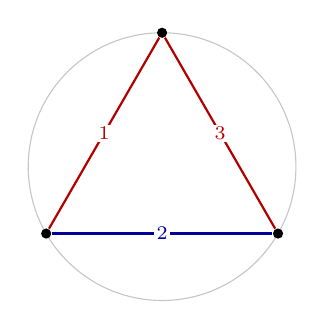
\begin{tikzpicture}[scale=1.0,
						pt/.style={circle, fill=black, inner sep=1.3pt},
						alice/.style={thick, red!70!black},
						bob/.style={thick, blue!60!black},
						lbl/.style={midway, fill=white, inner sep=0.8pt, font=\scriptsize}]
					\def\R{1.7}
					\draw[gray!45] (0,0) circle (\R);
					\foreach \i in {0,...,2} {
						\node[pt] (P\i) at ({90 + 120*\i}:\R) {};
					}
					\draw[alice] (P0) -- (P1) node[lbl] {1};
					\draw[bob] (P1) -- (P2) node[lbl] {2};
					\draw[alice] (P2) -- (P0) node[lbl] {3};
				\end{tikzpicture}
				\caption{$n=3$: the game lasts exactly $2(3)-3=3$ moves, so Alice (red) plays moves $1$ and $3$ and makes the last one.}
				\label{fig:chords-n3}
			\end{subfigure}
			\hfill
			\begin{subfigure}[b]{0.48\textwidth}
				\centering
				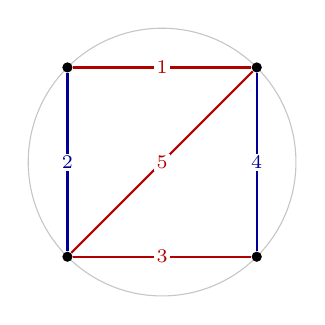
\begin{tikzpicture}[scale=1.0,
						pt/.style={circle, fill=black, inner sep=1.3pt},
						alice/.style={thick, red!70!black},
						bob/.style={thick, blue!60!black},
						lbl/.style={midway, fill=white, inner sep=0.8pt, font=\scriptsize}]
					\def\R{1.7}
					\draw[gray!45] (0,0) circle (\R);
					\foreach \i in {0,...,3} {
						\node[pt] (P\i) at ({45 + 90*\i}:\R) {};
					}
					\draw[alice] (P0) -- (P1) node[lbl] {1};
					\draw[bob] (P1) -- (P2) node[lbl] {2};
					\draw[alice] (P2) -- (P3) node[lbl] {3};
					\draw[bob] (P3) -- (P0) node[lbl] {4};
					\draw[alice] (P0) -- (P2) node[lbl] {5};
				\end{tikzpicture}
				\caption{$n=4$: the game lasts exactly $2(4)-3=5$ moves, so Alice (red) plays moves $1,3,5$ and makes the last one.}
				\label{fig:chords-n4}
			\end{subfigure}

			\vspace{1em}

			\begin{subfigure}[b]{0.48\textwidth}
				\centering
				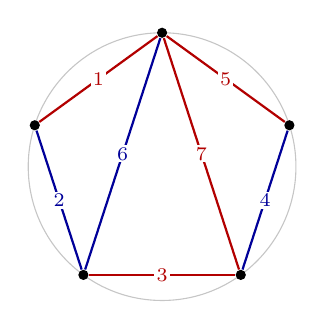
\begin{tikzpicture}[scale=1.0,
						pt/.style={circle, fill=black, inner sep=1.3pt},
						alice/.style={thick, red!70!black},
						bob/.style={thick, blue!60!black},
						lbl/.style={midway, fill=white, inner sep=0.8pt, font=\scriptsize}]
					\def\R{1.7}
					\draw[gray!45] (0,0) circle (\R);
					\foreach \i in {0,...,4} {
						\node[pt] (P\i) at ({90 + 72*\i}:\R) {};
					}
					\draw[alice] (P0) -- (P1) node[lbl] {1};
					\draw[bob] (P1) -- (P2) node[lbl] {2};
					\draw[alice] (P2) -- (P3) node[lbl] {3};
					\draw[bob] (P3) -- (P4) node[lbl] {4};
					\draw[alice] (P4) -- (P0) node[lbl] {5};
					\draw[bob] (P0) -- (P2) node[lbl] {6};
					\draw[alice] (P0) -- (P3) node[lbl] {7};
				\end{tikzpicture}
				\caption{$n=5$: the game lasts exactly $2(5)-3=7$ moves, so Alice (red) plays moves $1,3,5,7$ and makes the last one.}
				\label{fig:chords-n5}
			\end{subfigure}
			\hfill
			\begin{subfigure}[b]{0.48\textwidth}
				\centering
				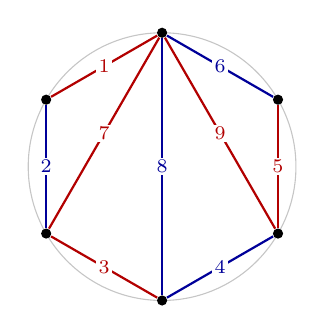
\begin{tikzpicture}[scale=1.0,
						pt/.style={circle, fill=black, inner sep=1.3pt},
						alice/.style={thick, red!70!black},
						bob/.style={thick, blue!60!black},
						lbl/.style={midway, fill=white, inner sep=0.8pt, font=\scriptsize}]
					\def\R{1.7}
					\draw[gray!45] (0,0) circle (\R);
					\foreach \i in {0,...,5} {
						\node[pt] (P\i) at ({90 + 60*\i}:\R) {};
					}
					\draw[alice] (P0) -- (P1) node[lbl] {1};
					\draw[bob] (P1) -- (P2) node[lbl] {2};
					\draw[alice] (P2) -- (P3) node[lbl] {3};
					\draw[bob] (P3) -- (P4) node[lbl] {4};
					\draw[alice] (P4) -- (P5) node[lbl] {5};
					\draw[bob] (P5) -- (P0) node[lbl] {6};
					\draw[alice] (P0) -- (P2) node[lbl] {7};
					\draw[bob] (P0) -- (P3) node[lbl] {8};
					\draw[alice] (P0) -- (P4) node[lbl] {9};
				\end{tikzpicture}
				\caption{$n=6$: the game lasts exactly $2(6)-3=9$ moves, so Alice (red) plays moves $1,3,5,7,9$ and makes the last one.}
				\label{fig:chords-n6}
			\end{subfigure}
			\caption{One possible play for $n=3,4,5,6$, with chords numbered in the order they are drawn and coloured by player (Alice red, Bob blue). Any other sequence of legal moves also terminates in a triangulation with $n$ sides and $n-3$ diagonals, hence after the same odd number $2n-3$ of moves.}
			\label{fig:chords-small-cases}
		\end{figure}
	\end{solution}

